% LaTeX-Vorlage zur Erstellung einer Abschlussarbeit in der Fakultät Elektrotechnik, Medien und Informatik an der OTH Amberg-Weiden
% Diese Vorlage entstand im Rahmen des Kurses "LaTeX fürs Studium"
% Aktuelle Version: v0.03
% Stand: 11.21.2024
%
% Changelog:
% v0.03: Nov.2024, Anpassung der Vorlage:
% + Übernahme des neuen Corporate Design
% + Einfügen von biblatex
%
% v0.02: 06.08.2015, Anpassung der Vorlage:
% + Persönliche Informationen (Vorname, Name, Titel usw.) werden direkt in die PDF-Dokumenteinstellungen übernommen
% + Korrektur der Verlinkung von Abbildungs- und Tabellenverzeichnis aus dem Inhaltsverzeichnis (phantomsection) bzw. deren Seitenzahl
%   Besten Dank für diesen Hinweis an Jan-Olaf Becker
% + Anpassung des Namens der Fakultät nach deren Umbenennung
%
% v0.01: 14.03.2012, Erstellung der Vorlage

\documentclass[12pt,oneside]{report}
\usepackage[T1]{fontenc}		% Einstellungen fuer Umlaute usw.
\usepackage[utf8x]{inputenc}
% \usepackage[ngerman]{babel}
\usepackage[english]{babel}
\usepackage[style=numeric]{biblatex}
\addbibresource{General.bib}
\addbibresource{Zotero.bib}
\addbibresource{RL.bib}
\addbibresource{chapter4/04_InstructRobots.bib}
\addbibresource{chapter4/04_DataProblem.bib}
\addbibresource{chapter5/chapter5.bib}
\addbibresource{chapter6/chapter6.bib}
\addbibresource{chapter7/chapter7.bib}
\addbibresource{chapter8/chapter_08.bib}
 
\usepackage{parskip}			% Einstellungen fuer Absaetze: Abstand statt Einrueckung

\usepackage[a4paper,			% Papierformat A4
	    left=2.5cm,				% linker Rand
	    right=2.5cm,			% rechter Rand
	    top=1.5cm,				% oberer Rand
	    bottom=1.5cm,			% unter Rand
	    marginparsep=5mm,		% Abstand der Randnotizen
	    marginparwidth=10mm, 	% Breite der Randnotizen
	    headheight=7mm,			% Hoehe der Kopfzeile
	    headsep=1.2cm,			% Abstand der Kopfzeile
	    footskip=1.5cm,			% Abstand der Fusszeile
	    includeheadfoot]{geometry}

\usepackage{fancyhdr}						% Konfiguration von Kopf- und Fusszeilen
\pagestyle{fancy}							% Seitenstil 'fancy'
\fancyhf{}									% vorhandene Einstellungen loeschen
\setlength{\headwidth}{\textwidth}			% Kopf- und Fusszeile so breit wie der Haupttext
\fancyfoot[R]{\thepage} 					% Festlegung des Seitenstils: Seitenzahlen in der Fusszeile rechts
\fancyfoot[L]{\leftmark}					% Kapitelnr. und -Bezeichnung in der Fusszeile links
\fancyhead[R]{\IhreArbeitEN}					% "Bachelorarbeit" in der Kopfzeile rechts
\fancyhead[L]{\IhrVorname\ \IhrNachname}	% Vorname und Name in der Kopfzeile links
\renewcommand{\chaptermark}[1]{			% Definition der Ausgabe des Kapitels
  \markboth{Chapter \thechapter. #1}{}}
\renewcommand{\headrulewidth}{0.5pt}		% Trennlinie zwischen Kopfzeile und Haupttext
\renewcommand{\footrulewidth}{0.5pt}		% Trennlinie zwischen Haupttext und Fusszeile
\fancypagestyle{plain}{					% Anpassung des Seitenstils 'plain' bei Beginn neuer Kapitel
  \fancyhf{}								% Vorbelegung loeschen
  % \fancyfoot[C]{\thepage}					% Seitenzeilen in der Fusszeile mittig
  % \fancyhead[R]{\IhreArbeit}				% "Bachelorarbeit" in der Kopfzeile rechts
  % \fancyhead[L]{\IhrVorname\ \IhrNachname}	% Vorname und Name in der Kopfzeile links


  \fancyfoot[LE,RO]{\thepage}                
  \fancyfoot[LO,RE]{\nouppercase\leftmark}
  \fancyhead[R]{\IhreArbeitEN}					        % "Bachelorarbeit" in der Kopfzeile rechts
  \fancyhead[L]{\IhrVorname\ \IhrNachname}	  % Vorname und Name in der Kopfzeile links

}



\setcounter{secnumdepth}{3} 
\setcounter{tocdepth}{3}


\usepackage{titlesec}
\titleformat{\paragraph}
{\normalfont\normalsize\bfseries}{\theparagraph}{1em}{}
\titlespacing*{\paragraph}
{0pt}{3.25ex plus 1ex minus .2ex}{1.5ex plus .2ex} 
% The last number (1.5ex) creates the vertical space below the heading


\usepackage{amsmath}			% Pakete fuer den Mathematikmodus
\usepackage{amssymb}
\usepackage[intlimits]{empheq}

\usepackage[sc]{mathpazo}		% Schriftart Palatino fuer Haupttext und Mathematikmodus
\usepackage{pifont}				% zusaetzliche Symbole

\usepackage[format=hang,		% Einstellung fuer Bildunterschriften
            font={footnotesize},
            labelfont={bf},
            margin=1cm,
            aboveskip=5pt,
            position=bottom]{caption}

\usepackage{graphicx}							% Einbinden von Graphiken
\usepackage[svgnames,cmyk,table,hyperref]{xcolor} 	% Verwendung von Farben
\usepackage{tikz}								% Erstellen von Grafiken
\usetikzlibrary{positioning,arrows,plotmarks} % TikZ-Bibliotheken
%\usepackage{pgfplots}                           % Darstellung von Plots, Funktionen, Graphen usw.
\usepackage{subfigure}
%
% Weitere Pakete
%
%\usepackage{listings}			% Darstellung von Quellcode
%\lstset{language=Python, basicstyle=\ttfamily, numbers=none}
%
%\usepackage[european, siunitx]{circuitikz}	% Darstellung von Schaltungen
%
%\usepackage{enumerate}			% Formatierung nummerierter Listen

\usepackage{microtype,relsize}					% Wird verwendet, um Nachnamen auf Titelseite gesperrt darzustellen
\newcommand*{\Sperren}[1]{\textls*[100]{#1}}

%
% Persoenliche Angaben
%
\newcommand*{\IhrVorname}{Sebastian}
\newcommand*{\IhrNachname}{Weidner}
\newcommand*{\IhrStudiengang}{Bachelor Künstliche Intelligenz}
\newcommand*{\IhreArbeit}{Bachelorarbeit}
\newcommand*{\IhreArbeitEN}{Bachelor Thesis}
\newcommand*{\IhrTitelDE}{Imitation Learning unter Verwendung videokonditionierter Policies für visuell gesteuertes Roboterverhalten}
\newcommand*{\IhrTitelEN}{Imitation Learning using Video-Conditioned Policies for Visually Guided Robotic Behavior}
\newcommand*{\IhrBearbeitungszeitraumVON}{20. Januar 2026}
\newcommand*{\IhrBearbeitungszeitraumBIS}{20. Juni 2026}
\newcommand*{\IhrErstpruefer}{Prof. Dr.-Ing. Christian Bergler}
\newcommand*{\IhrZweitpruefer}{Prof. Dr. phil. Tatyana Ivanovska}
\newcommand*{\IhreFirma}{OTH Amberg-Weiden}
\newcommand*{\IhrFirmenbetreuer}{Prof. Dr.-Ing. Christian Bergler}
\newcommand*{\IhreZusammenfassungDe}{%
Lorem ipsum dolor sit amet, consetetur sadipscing elitr, sed diam nonumy eirmod tempor invidunt ut labore et dolore magna aliquyam erat, sed diam voluptua. At vero eos et accusam et justo duo dolores et ea rebum. Stet clita kasd gubergren, no sea takimata sanctus est Lorem ipsum dolor sit amet. Lorem ipsum dolor sit amet, consetetur sadipscing elitr, sed diam nonumy eirmod tempor invidunt ut labore et dolore magna aliquyam erat, sed diam voluptua. At vero eos et accusam et justo duo dolores et ea rebum. Stet clita kasd gubergren, no sea takimata sanctus est Lorem ipsum dolor sit amet.
}

\newcommand*{\IhreSchluesselwoerterDe}{\LaTeX, Textsatz, Formeln, Graphiken}
\newcommand*{\IhreZusammenfassungEn}{%
Lorem ipsum dolor sit amet, consetetur sadipscing elitr, sed diam nonumy eirmod tempor invidunt ut labore et dolore magna aliquyam erat, sed diam voluptua. At vero eos et accusam et justo duo dolores et ea rebum. Stet clita kasd gubergren, no sea takimata sanctus est Lorem ipsum dolor sit amet. Lorem ipsum dolor sit amet, consetetur sadipscing elitr, sed diam nonumy eirmod tempor invidunt ut labore et dolore magna aliquyam erat, sed diam voluptua. At vero eos et accusam et justo duo dolores et ea rebum. Stet clita kasd gubergren, no sea takimata sanctus est Lorem ipsum dolor sit amet.
}
\newcommand*{\IhreSchluesselwoerterEn}{\LaTeX, Textsatz, Formeln, Graphiken}


\usepackage[bookmarks, raiselinks, pageanchor, % PDF-Einstellungen
            hyperindex, colorlinks,
            citecolor=black, linkcolor=black,
            urlcolor=black, filecolor=black,
            menucolor=black]{hyperref}
\hypersetup{pdftitle={\IhrTitelDE},%
            pdfauthor={\IhrVorname\ \IhrNachname},%
            pdfsubject={\IhreArbeit},%
            pdfkeywords={\IhreSchluesselwoerterDe}}


%Linebreaks of urls in bibliography
\usepackage{url}
\setcounter{biburllcpenalty}{7000}
\setcounter{biburlucpenalty}{8000}



\usepackage{minitoc}
\dominitoc
\setcounter{minitocdepth}{2}
\setcounter{secnumdepth}{2}
\setcounter{tocdepth}{2}
\addto{\captionsenglish}{
  \renewcommand{\mtctitle}{} % Remove "Contents" from minitoc title
}


%
% Beginn des Textteils
%
\begin{document}
  \pagenumbering{roman}
  \begin{titlepage}					% Titelseite
    \thispagestyle{empty}
    \begin{center}
      \Large
      Ostbayerische Technische Hochschule Amberg-Weiden\\
      Fakultät Elektrotechnik, Medien und Informatik\\[1cm]
      Studiengang \IhrStudiengang\\[1cm]
      \textbf{\IhreArbeit}\\[1cm]
      von\\[1cm]
      \IhrVorname\ \Sperren{\textbf{\IhrNachname}}\\[1cm]
      \textbf{\IhrTitelDE}\\[1cm]
      \IhrTitelEN
    \end{center}
  \end{titlepage}
  \clearpage
  \thispagestyle{empty}			% 1. Seite soll eine Leerseite sein (dazu muss ein Trick verwendet werden)
  \mbox{}
  \clearpage
  \thispagestyle{empty}			% 2. Seite wie Titelseite, aber mit zusaetzlichen Angaben
  \begin{center}
    \Large
    Ostbayerische Technische Hochschule Amberg-Weiden\\
    Fakultät Elektrotechnik, Medien und Informatik\\[1cm]
    Studiengang \IhrStudiengang\\[1cm]
    \textbf{\IhreArbeit}\\[1cm]
    von\\[1cm]
    \IhrVorname\ \Sperren{\textbf{\IhrNachname}}\\[1cm]
    \textbf{\IhrTitelDE}\\[1cm]
    \IhrTitelEN
  \end{center}
  \vspace*{5cm}
  \begin{tabbing}
    \underbar{Bearbeitungszeitraum:}\qquad\= von\qquad\=\IhrBearbeitungszeitraumVON\\
                                          \> bis      \>\IhrBearbeitungszeitraumBIS
  \end{tabbing}
  \vspace*{1cm}
  \underbar{1. Prüfer:}\qquad\IhrErstpruefer\par
  \underbar{2. Prüfer:}\qquad\IhrZweitpruefer
  \clearpage
  % formblatt_selbststaendigkeitserklaerung.tex
%

\thispagestyle{empty}				% Formblatt nach ASPO
\vspace*{-3cm}
\begin{minipage}{0.60\textwidth}
  \mbox{}
  \hfill

\end{minipage}
\begin{minipage}{0.4\textwidth}

\includegraphics[height=2.5cm]{logo.jpg}
\end{minipage}
\vspace{1.5cm}

Eigenständigkeitserklärung gemä\ss \: \S \: 27 (8) ASPO\\
\rule[1ex]{\textwidth}{0.5pt}
\vspace*{0.5cm}
\begin{tabbing}
  Name und Vorname\\
  der Studentin/des Studenten:\qquad\=\textbf{\IhrNachname, \IhrVorname}\\[1cm]
  Studiengang:                      \>\textbf{\IhrStudiengang}
\end{tabbing}
\rule[1ex]{\textwidth}{0.5pt}
\vspace*{0.5cm}
Ich bestätige, dass ich die \IhreArbeit\ mit dem Titel:
\begin{center}
  \textbf{\IhrTitelDE}
\end{center}
\vspace*{0.5cm}
selbständig verfasst, noch nicht anderweitig für Prüfungszwecke vorgelegt, keine anderen als die angegebenen Quellen oder Hilfsmittel benutzt sowie wörtliche und sinngemäße Zitate als solche gekennzeichnet habe.\\[0.5cm]
\rule[1ex]{\textwidth}{0.5pt}
\begin{tabbing}
  Datum:\hspace{2cm}\=\today\\[1cm]
  Unterschrift:\>
\end{tabbing}
\rule[1ex]{\textwidth}{0.5pt}
\clearpage
		% 3. Seite: Formblatt Bestaetigung nach Paragraph 12 APO
  % formblatt_summary.tex
%

\thispagestyle{empty}				% Formblatt Zusammenfassung
\begin{minipage}{0.65\textwidth}
  \mbox{}
  \hfill
\end{minipage}
\begin{minipage}{0.35\textwidth}
  
\includegraphics[height=2.5cm]{logo.jpg}
\end{minipage}
\IhreArbeit\ Zusammenfassung\\
\rule[1ex]{\textwidth}{0.5pt}
\vspace*{0.5cm}
\begin{tabular}{lp{6.5cm}}
  \hspace*{-1ex}Student: & \textbf{\IhrNachname, \IhrVorname}\\
  \hspace*{-1ex}Studiengang: & \IhrStudiengang\\
  \hspace*{-1ex}Professor: & \IhrErstpruefer\\
  \hspace*{-1ex}Durchgeführt in Hochschule: & \IhreFirma\\
  \hspace*{-1ex}Betreuer in Hochschule: & \IhrFirmenbetreuer\\
  \hspace*{-1ex}Ausgabedatum: & \IhrBearbeitungszeitraumVON\\
  \hspace*{-1ex}Abgabedatum: & \IhrBearbeitungszeitraumBIS\\
  % \multicolumn{2}{l}{\hspace*{-1ex}Ausgabedatum: \IhrBearbeitungszeitraumVON\qquad\qquad Abgabedatum: \IhrBearbeitungszeitraumBIS}
\end{tabular}\par


\rule[1ex]{\textwidth}{0.5pt}
Title:
\begin{center}
  \textbf{\IhrTitelEN}
\end{center}
\vspace*{0.5cm}
\rule[1ex]{\textwidth}{0.5pt}

\subsection*{Abstract}
\IhreZusammenfassungEn\\[0.1cm]
\subsection*{Keywords} \IhreSchluesselwoerterEn


% \rule[1ex]{\textwidth}{0.5pt}
% Titel:
% \begin{center}
%   \textbf{\IhrTitelDE}
% \end{center}
% \vspace*{0.5cm}
% \rule[1ex]{\textwidth}{0.5pt}
\subsection*{Zusammenfassung}
\IhreZusammenfassungDe\\[0.1cm]
\subsection*{Schlüsselwörter} \IhreSchluesselwoerterDe




\clearpage			% 4. Seite: Formblatt Zusammenfassung
  \tableofcontents
  \newpage
  \chapter*{Symbole, Formelzeichen und Einheiten}
  \newpage
  \pagenumbering{arabic}
  \chapter{Introduction }

\section{Motivation}
Roboter werden zukünftig eine Schlüsselrolle in zahlreichen Anwendungsfeldern einnehmen. Be-reits heute steigt der Einsatz von Robotersystemen in der industriellen Produktion kontinuierlich an, da diese insbesondere monotone, einfache und repetitive Aufgaben effizient und zuverlässig übernehmen können. Trotz der teilweisen sehr hohen Anschaffungskosten, investieren immer mehr Unternehmen in die Integration von Roboter in Ihre Produktionslinien. 
Die Vorteile liegen dabei vor allem in der hohen Verfügbarkeit und Planbarkeit: Nach der Inbe-triebnahme fallen nur noch geringe laufende Betriebskosten an, die sich primär auf Energiever-brauch in From von Strom- und Wartungskosten beschränken. Darüber hinaus können Roboter unabhängig von der Arbeitszeit 24h, 7 Tage die Woche betrieben werden und liefern eine gleich-bleibende Qualität. Dies ermöglicht eine hohe Prozessstabilität sowie eine signifikante Steigerung der Produktivität. Im Gegensatz zu menschlichen Arbeitskräften, werden Roboter nicht krank, nehmen nicht an einen Gewerkschaftsstreik teil und es müssen auch keine Sonderzahlungen in Form von Nacht-, Wochenend- und Feiertagszuschlägen geleistet werden.
Grundsätzlich lassen sich Robotersysteme hinsichtlich ihrer Programmierung in zwei Kategorien einteilen. In der industriellen Praxis dominieren derzeit statisch programmierte Roboter, die für klar definierte Aufgaben in strukturierten Umgebungen eingesetzt werden. Sie haben feste Bewe-gungsabläufe und können sich nur in geringem Maße mithilfe integrierter intelligenter Sensoren an ihre Umgebung bzw. an die jeweilige Aufgabe anpassen. Solche Systeme sind besonders effi-zient in standardisierten Produktionsprozessen, stoßen jedoch an ihre Grenzen, sobald sich die Umgebung oder die Anforderungen ändern.
Im Gegensatz dazu gewinnen intelligente Robotersysteme zunehmend an Bedeutung. Diese sind in der Lage, auf Veränderungen in ihrer Umgebung zu reagieren und ihr Verhalten adaptiv anzu-passen. Insbesondere durch den Einsatz von Künstlicher Intelligenz eröffnen sich neue Möglich-keiten, komplexe und unstrukturierte Aufgaben zu bewältigen. 
Zentrale Herausforderungen bestehen jedoch hierdabei in der robusten Ausführung vielfältiger Szenarien sowie in der Fähigkeit, auf neue Objekte, Umgebungen und Aufgaben zu generalisieren. Die heute eingesetzten intelligenten Robotersysteme, bzw. deren zugrunde liegenden KI-Modelle sind oftmals stark auf ihre jeweilige Aufgabe und die Zielumgebung spezialisiert, bzw. trainiert worden.
Aufgaben, die nicht im Trainingsdatensatz enthalten sind, können häufig nicht zuverlässig ausge-führt werden. Ebenso treten Probleme auf, wenn gelernte Aufgaben in grundlegend verschiedenen Umgebungen ausgeführt werden sollen. Der Grund hierfür liegt in der Art und Weise, wie die zugrunde liegenden KI-Modelle trainiert werden: Die Trainingsdaten sind in der Regel stark auf eine spezifische Aufgabe und Umgebung zugeschnitten. Eine Erhöhung der Datenvielfalt führt dabei häufig zu einem Zielkonflikt, da sie mit einer geringeren Genauigkeit bei der Ausführung einzelner Aufgaben einhergehen kann. 
Selbst wenn man ein großes generalisierendes Roboter KI-Modell entwickeln möchte, stellt der Mangel an geeigneten und vielfältigen Roboter-Trainingsdaten ein gravierendes Problem dar.
Klassische, aufgabenspezifische Trainingsansätze stoßen hierbei aufgrund mangelnder Skalierbar-keit und Flexibilität an ihre Grenzen. Aktuelle Forschungsansätze verfolgen daher das Ziel, Robo-tern ein visuelles und semantisches Aufgabenverständnis zu vermitteln, sodass sie Handlungen aus hochdimensionalen Eingaben wie Videos oder Bildern ableiten können. Dadurch können neue Datenquellen für das Training des Roboters herangezogen werden. Mit einem visuellen und se-mantischen Verständnis können beispielsweise (menschliche) Videos von YouTube im Training verwendet werden. Diese beinhalten viele verschiedene Handlungen und Ausführungsformen ver-schiedenster Aufgaben, die ein generalisierendes Roboter KI-Modell brauchen würde. Imitation Learning ist ein vielversprechender Ansatz in diesem Kontext, der in dieser Arbeit genauer unter-sucht wird.

% ToDo: evtl. in Project goal einfügen und Thesis schreiben anstatt Project
Beim Imitation Learning geht es darum, den Roboter seine Aufgabe mithilfe eines (menschlichen) Demonstrationsvideos beizubringen (z.B. das Stapeln von Würfeln, oder das Greifen von Objek-ten). Beim traditionellen Ansatz muss ein Roboter auf die jeweilige Aufgabe mit viel Aufwand bzw. mit vielen Roboter trajectory Datensätzen trainiert werden.

\section{Project Goal}
Ziel dieser Arbeit ist es eine Einführung in das Thema Robotic mit Imitation Learning zu liefern. Die Arbeit gliedert sich in zwei Teile. 
Dabei werden zuerst die Grundlagen der Robotik erläutert und anschließend technisch in das Thema Intelligente Robotik mit dem Fokus Imitation Learning eingeführt. Abgerundet wird der erste Teil mit einem Literaturüberblick, über ausgewählte Imitation Learning Ansätze, die dort näher untersucht werden.
Im zweiten Teil dieser Arbeit wird ein Open-Source Imitation Learning Modell experimentell auf einen realen Roboterarm implementiert. Die Erstmalige Inbetriebnahme des Roboters und das Setup, wie ein KI-Modell zur Ausführung auf den Roboter gebracht werden kann, gehört auch dazu. Ziel ist es, den Roboter zu befähigen, einfache Manipulationsaufgaben, beispielsweise das Stapeln von Würfeln, allein auf Basis menschlicher Demonstrationsvideos zu erlernen und auszu-führen. Die Leistungsfähigkeit des vorgeschlagenen Ansatzes wird anschließend experimentell auf dem realen Robotersystem untersucht und evaluiert.



Beim Imitation Learning geht es darum, den Roboter seine Aufgabe mithilfe eines (menschlichen) Demonstrationsvideos beizubringen (z.B. das Stapeln von Würfeln, oder das Greifen von Objek-ten). Beim traditionellen Ansatz muss ein Roboter auf die jeweilige Aufgabe mit viel Aufwand bzw. mit vielen Roboter trajectory Datensätzen trainiert werden.
Beim Imitation Learning geht es darum, den Roboter seine Aufgabe mithilfe eines (menschlichen) Demonstrationsvideos beizubringen. Dabei nimmt eine Kamera ein Video von der jeweiligen Person auf, die eine bestimmte Aufgabe ausübt. Anschließend wird dem Roboter-KI-Modell das Demonstrationsvideo der Aufgabe gezeigt, welches wiederum den Roboter entsprechend steuert, um die jeweilige Aufgabe in seiner Umgebung auszuführen.



\section{Outline of the Thesis}
This thesis examine imitation learning as a promising approach for enabling robots to acquire complex skills from demonstrations and move toward the long-term goal of general-purpose robotic intelligence.
\acp{LLM} have demonstrated that training powerful architectures on vast and diverse datasets can lead to remarkable generalization capabilities, enabling systems to solve tasks for which they were never explicitly trained. A central goal of imitation learning is to bring similar capabilities to robotic systems by leveraging the enormous amount of video data available on the internet.
% Imitation learning represents one of the most promising approaches for transferring the success of large-scale machine learning to robotics. 

Chapter \ref{chap:Foundations} introduced the fundamental concepts of imitation learning and distinguished between two major paradigms: Behavior Cloning and Learning from Videos (LfV). 
% While Behavior Cloning relies on demonstrations containing explicit action labels, Learning from Videos seeks to exploit the vast amount of action-free video data available online, offering a scalable alternative for robot learning.

Chapter \ref{chap:GeneralistRobotsAndTheDataBottleneck} discussed the overarching objective of robotics research: the development of generalist robots capable of performing a wide range of tasks in unstructured and previously unseen real-world environments. A major obstacle to this vision is the robotics data bottleneck, which arises from the limited availability of large, diverse, and high-quality robotic datasets. Internet videos represent a potential solution due to their abundance and diversity. However, their use introduces additional challenges related to the transfer of visual knowledge to robotic systems.

A prerequisite for effective human-robot interaction is the ability to communicate goals and intentions to robotic agents. Therefore, chapter \ref{chap:WaysToInstructRobots} examined how robots can be instructed and guided to perform desired tasks. 
% the thesis examined different approaches for task specification and human-robot interaction, highlighting how robots can be instructed through demonstrations, language, and other forms of guidance.
% Various forms of task specification and human-robot interaction were presented.

Chapter \ref{chap:LearningFromVideosDataModalityAndChallenges} focused on the central research questions of Learning from Videos: how relevant knowledge can be extracted from internet videos and how this knowledge can subsequently be transferred to robotic systems for policy learning and control. Video Foundation Models were introduced as a powerful tool for extracting semantic and behavioral information from large-scale video data. Two major challenges were identified in the transfer process: the absence of action labels and the distribution shift between human videos and robotic observations. To address these challenges, alternative action representations are employed to relabel action-free video data, enabling robots to learn from demonstrations that do not contain explicit control signals.

Chapter \ref{chap:RobotLearningObjectivesForUnderstandingDemonstrationVideos} explored the role of robust video understanding in \ac{IL}. Learning manipulation skills from video requires more than simple action recognition: (1) It demands meaningful representations of the environment, (2) an understanding of object affordances and human-object interactions, (3) recognition of human activities, and (4) accurate modeling of fine-grained hand movements.
These capabilities form the basis for a general-purpose robot that can interpret human demonstrations.
% These capabilities form the basis of a general-purpose robot capable of understanding human demonstrations.
% These capabilities form the foundation for a general-purpose robot designed to interpret human demonstrations.




Chapter \ref{chap:RobotLearningApproaches} focused on approaches for learning coherent robot models from video data. 
(1) The chapter first introduced foundational perception and representation learning methods and techniques. 
(2) It then discussed both RL-based and imitation learning approaches, highlighting their respective strengths and limitations. 
(3) Hybrid methods, which combine the structured guidance and sample efficiency of imitation learning with the exploration and optimization capabilities of reinforcement learning. Special attention was given to the intersection of \acf{LfV} and \acf{RL}, demonstrating how knowledge extracted from videos can be used to improve policy learning and enhance the sample efficiency of RL algorithms.
(4) Last but not least, the chapter presented multi-modal learning approaches and \acf{VLA} models and the three Architecturial paradigms, including sensorimotor, world-model-based, and affordance-based architectures. \ac{VLA} models represent currently the state of the art in video-based robot learning.

Chapter \ref{chap:ChallengesAndFutureDirections} examined the major challenges and future research directions in \ac{IL} and video-based robotic learning. Despite significant advances in recent years, the development of robust and generalizable robotic systems remains constrained by several fundamental limitations, including data availability, computational scalability, domain transfer and efficient policy learning. These challenges highlight the gap between current research systems and the long-term goal of general-purpose robotic intelligence. 
At the same time, emerging approaches such as diffusion-based policies, world models, and causally-aware learning systems offer promising opportunities for overcoming these limitations and improving the adaptability, reasoning capabilities, and generalization performance of future robotic agents.


Finally in Chapter \ref{chap:SelectedApproaches} of the literature overview, selected \ac{IL} approaches deployed on real robotic systems were examined to provide practical insight into the theoretical concepts discussed throughout the thesis. These examples illustrated how \ac{IL} can enable robots to acquire complex manipulation and control skills directly from video demonstrations.

The second part of the thesis focused on the practical implementation of an \ac{IL} approach on a real robotic system, which is examined in Chapter \ref{chap:ExperimentsOnARealRobot}.
  \chapter{Fundamentals}
\label{chap:Foundations}
\minitoc
This chapter provides an overview of the key concepts and theories that form the foundation of the following chapters. 





% \section{Glossary}
% \paragraph{Agent:}
% An agent is an entity that learns to perform a specific behavior through interaction with its environment. In the context of this work, the agent corresponds to the robot, which has to execute a given action or task. 

% \paragraph{Policy:}
% The policy can be interpreted as the brain of the agent, determining which action to take next in a given situation in order to achieve the task objective. In our example, the policy controls the robot's motion and actions.  

% Formally, a policy can be represented as  
% \begin{align}
% 	\pi_\theta(a \mid s)  
% \end{align}
% which defines a probability distribution over actions $a$, conditioned on the current state $s$. In other words, the policy specifies how likely the agent is to select a particular action given its current observation of the environment.  

% In the classical meaning, the action $a$ corresponds for example to a robot command, such as moving the gripper to a target position $(x, y, z)$ or setting a joint angle to a specific value with a defined velocity. The state $s$ represents the agent's observation, which may include, for example, a sequence of recent camera images (e.g., the last four frames) as well as additional sensor inputs such as proprioceptive signals.

% \paragraph{Robot Trajectory:}

% A robot trajectory describes how the robot moves from a starting state to a target state, including position, orientation and, if applicable, speeds, accelerations and forces acting on the robot. A robot trajectory is a temporal sequence of actions and the resulting robot states.

% \paragraph{Inference:}
% Inference refers to the process of using a trained model to make predictions or decisions based on new, unseen data. In the context of robotics, inference involves the robot applying its learned policy in real world or simulation to execute a given task.

% \paragraph{Annotation:}

% Annotating refers to the process of labeling data, in which data is enriched with additional information. For example, this may include assigning class labels, marking target objects in images, or labeling states and actions within robot trajectories. Annotated, or labeled, data forms the foundation for supervised learning approaches.


% \section{Machine Learning: Core Categories}
\section{Core Learning Paradigms in Machine Learning}
There are various approaches to training an \ac{AI} model for a robot. These involve methods from the four core \ac{ML} categories, which can also be combined.

\paragraph{Supervised Learning:}

In supervised learning, a model is trained using labeled training data. This means that, for the input data, the output data to be predicted are known. The goal is to train a model that correctly predicts the output data and makes reliable predictions on unseen data. 



\textit{Weakly supervised learning} is a \ac{ML} approach that learns a model from a combination of labeled and unlabeled data, or from data with noisy or imprecise labels. This allows models to leverage large amounts of unlabeled data while still benefiting from the guidance provided by the available labeled data. This approach is particularly relevant in robotics, where obtaining fully annotated data can be costly and time-consuming. 




\paragraph{Unsupervised Learning:}
In contrast to supervised learning, unsupervised learning uses unlabeled data for model training. The model tries to recognize structures, patterns or relationships in the data on its own. 

\textit{Self-Supervised Learning} is a \ac{ML} approach where the model learns to predict parts of the input data from other parts of the same data and therefore does not require external labels. The model generates its own supervisory signal from the data itself. For example, \acp{LLM} learn to predict the next word in a sentence based on the surrounding context, where the correct target words are already contained within the training data. Similarly, in computer vision, a model may learn to reconstruct masked regions of an image, with the original image providing the target information.
% In robotics, self-supervised learning can be used to learn representations of the environment or to predict future states based on current observations, enabling the robot to learn useful features and dynamics without the need for explicit annotations.


\paragraph{Semi-Supervised Learning:}
Semi-supervised learning is a combination of supervised and unsupervised learning. In this approach, a model is trained using a small amount of labeled data and a large amount of unlabeled data. The goal is to leverage the advantages of both approaches, particularly when annotating data is time-consuming or cost intensive. This is relevant in robotics, as the data used in that field is often difficult to label.


\paragraph{Reinforcement Learning:}

\ac{RL} differs fundamentally from the previously mentioned approaches. Instead of learning from fixed datasets, an agent actively interacts with its environment and tries to find out an optimal strategy to reach a defined goal. Through its actions, it influences the state of the environment and subsequently receives feedback in the form of rewards or penalties, see Figure \ref{fig:RLConzept} for a short overview. In the context of robotics, the robot is the agent.
The objective is to learn a strategy (= policy) that maximizes the cumulative reward over time for the given task.

\begin{figure}[!ht]
	\centering
	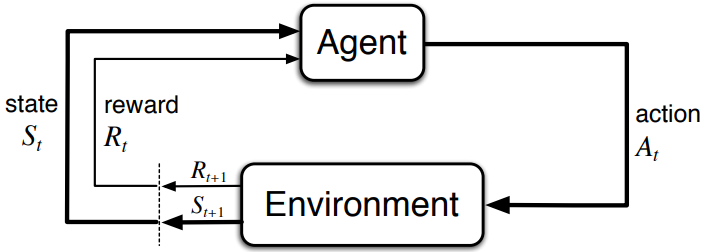
\includegraphics[width=0.6\linewidth]{./chapter3/media/RLConzept}
	\caption[Base concept of Reinforcement Learning]{Base concept of Reinforcement Learning: The Agent interacts with its environment and receives feedback in the form of rewards. Image source:~\cite{sutton2018reinforcement}.}
	\label{fig:RLConzept}
\end{figure}

The agent proceeds in its environment according to the trial-and-error principle to learn this optimal policy. Safety is a critical concern during training, as the agent may execute unpredictable actions while exploring the state space. For this reason, simulation environments are a central component of training and are frequently used for pre-training the policy. The policy is then subsequently often fine-tuned in the real-world environment. Through the trial and error, more efficient, unknown and creative solutions can be found that a human might not have come up with.










% Neuronale Netze

\section{Neural Networks}
Artificial Neural Networks are computational models inspired by the structure and functionality of biological brain and have become a fundamental component of modern machine learning. They are designed to learn complex relationships from data by approximating highly nonlinear functions and are therefore widely used in applications such as image recognition, natural language processing, forecasting and control systems. There exist various types of neural network architectures, including \acfp{CNN} or Transformer models, each tailored to specific types of data and tasks. The following sections provide an overview of the basic functionality of neural networks, their mathematical formulation and the training process.


\subsection{Neuron}
The basic element of an neural network is the neuron. The concept is motivated by biological neurons in the human brain, which communicate through electrochemical signals. In a simplified model, a biological neuron receives signals from other neurons, processes the received information and transmits an output signal~\cite{Lin2017ArtificialNN}. Artificial neurons mimic this behavior mathematically by combining several input values into a single output.

\paragraph{History}
The first mathematical model of an artificial neuron was proposed by McCulloch and Pitts in 1943~\cite{McCulloch1990ALC}. Their model consisted of a binary threshold unit that produced an output only when the weighted sum of its inputs exceeded a predefined threshold and established the foundations for later neural network research.
A major extension of this idea was introduced by Rosenblatt in 1958 with the perceptron~\cite{Rosenblatt1958ThePA}. The perceptron introduced trainable weights to the inputs and a learning rule, making it possible to adapt the model parameters directly from data. However, the perceptron still relied on a threshold-based activation, which produces a linear decision boundary and was therefore limited to linearly separable classification problems~\cite{Minsky1969AnIT}.
This limitation was highlighted by Minsky and Papert, who showed that a single perceptron cannot represent functions such as XOR~\cite{Minsky1969AnIT}. The development of multilayer neural networks together with differentiable activation functions later overcame this restriction. These advances made it possible to train networks with multiple layers and enabled the modern neural network architectures that are used in deep learning today.

\paragraph{Mathematical Formulation}
\begin{figure}[!h]
	\centering
	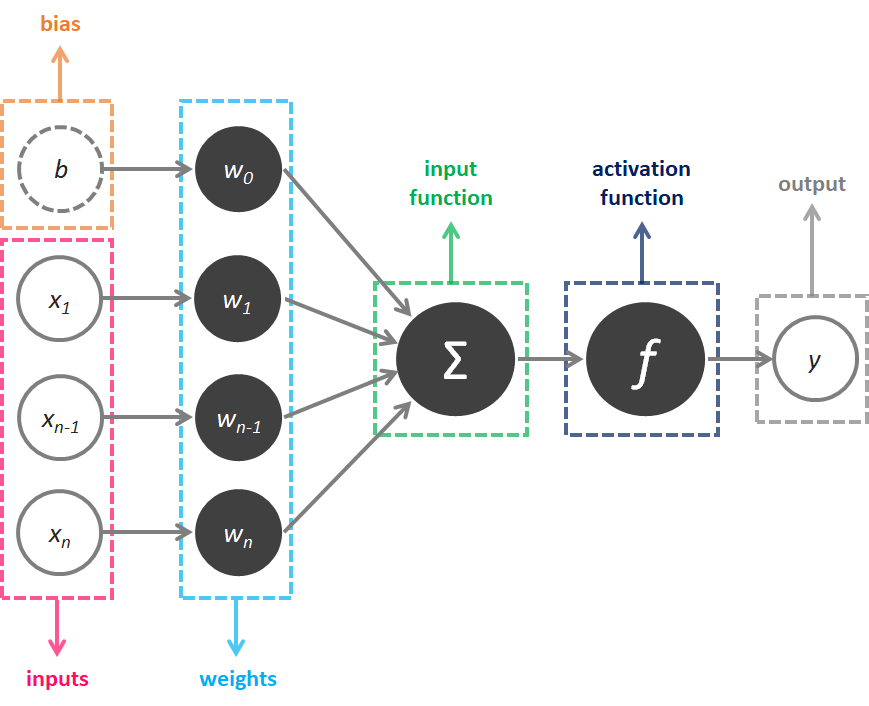
\includegraphics[width=0.55\linewidth]{./chapter2/media/NNNeuron2}
	\caption[Perceptron of an Artificial Neural Network]{Perceptron of an Artificial Neural Network. Image source:~\cite{yseYourGuidePerceptrons2024}.}
	\label{fig:NNIntroModernNeuron}
\end{figure}
A neuron receives an input vector $\mathbf{x}=[x_1,x_2,\ldots,x_n]^T$, where each vector element $x_i$ is associated with a trainable weight $w_i$ from the corresponding weight vector $\mathbf{w} = [w_1, w_2, \ldots, w_n]^T$. The neuron first computes a weighted sum of its inputs and adds a bias term $b$, see \autoref{fig:NNIntroModernNeuron}. The resulting pre-activation value is given by: 
% The weighted inputs are summed together with an optional bias term $(b)$, see \autoref{eq:perceptron}. 
\begin{equation}
    z = \sum_{i=1}^{n} w_i x_i + b
    \label{eq:neuron_scalar}
\end{equation}

The value $z$ represents a linear combination of the input features. To enable the modeling of non-linear relationships, an activation function $\phi(\cdot)$ is subsequently applied, yielding the neuron's output:

\begin{equation}
    y = \phi(z) = \phi\left(\sum_{i=1}^{n} w_i x_i + b\right)
    \label{eq:neuron_activation}
\end{equation}

Without the activation function, a composition of multiple neurons would still correspond to a single linear transformation and therefore could not represent complex non-linear patterns. Common activation functions used in modern neural networks include for example the GeLU, tanh and ReLU.




The weighted sum in \autoref{eq:neuron_scalar} can be expressed more compactly using vector notation and ending in the form of:
\begin{equation}
    y = \phi\!\left(\mathbf{w}^T \mathbf{x} + b\right)
	= \phi\!\left(
        \begin{bmatrix}
            w_1 & w_2 & \cdots & w_n
        \end{bmatrix}
        \begin{bmatrix}
            x_1 \\
            x_2 \\
            \vdots \\
            x_n
        \end{bmatrix}
        + b
    \right) 
    \label{eq:single_neuron}
\end{equation}

This vector formulation serves as the basis for the matrix representation of an entire neural network layer, where multiple neurons are evaluated simultaneously.

\subsection{Neural Networks}
A neural network is a collection of interconnected neurons organized into layers. 
The input layer receives the feature vector, while the output layer produces the final prediction. The hidden layers between the input and output layers perform intermediate computations that allow the network to learn increasingly abstract representations of the input data~\cite{Goodfellow-et-al-2016}.
The parameters of the network (the weights and biases) are learned from data using optimization algorithms such as gradient descent~\cite{Rumelhart1986LearningRB}. As universal function approximators, neural networks are capable of learning complex functions from data, which has made them a powerful tool across numerous applications in machine learning.
% Technically, neural networks are universal function approximators, enabling them to learn complex functions from data and making them a powerful tool for a wide range of applications in machine learning.


To understand the terminology: Artificial neural network is the broadest term, encompassing all brain-inspired, connectionist models. A feedforward neural network is a subcategory where information flows strictly in one direction (from input to output) without forming cycles, but its layers need not be fully connected~\cite{Goodfellow-et-al-2016}. The multilayer perceptron is a feedforward network with one or more fully connected (dense) hidden layers, where every neuron in one layer connects to every neuron in the next~\cite{Goodfellow-et-al-2016}. In a fully connected layer, every neuron is connected to every neuron in the subsequent layer~\cite{Goodfellow-et-al-2016}.
% Each layer consists of multiple neurons and the output of one layer serves as the input to the next layer.

% In general, a neural network consists of multiple interconnected neurons organized into layers
%  and the output of one layer serves as the input to the next layer. 

\paragraph{Multilayer Perceptron Network}
The most common form of such architectures is the \textit{\acf{MLP}}~\cite{Goodfellow-et-al-2016}. In an \ac{MLP}, information flows in one direction from the input layer through one or more fully connected hidden layers to the output layer, where each neuron in a layer receives the outputs of the neurons in the preceding layer as inputs. 
% The output of a layer therefore serves as the input to the next layer.

\begin{figure}[!h]
	\centering
	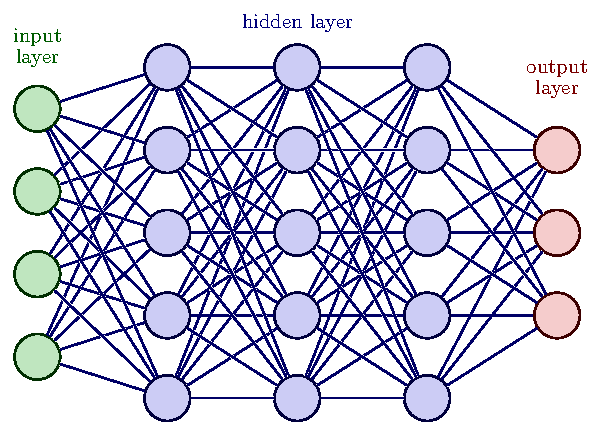
\includegraphics[width=0.55\linewidth]{./chapter2/media/NNNetwork}
	\caption[Neural Networks: Architecture]{Architecture of an Multilayer Perceptron Network. Circles represent perceptrons. Image source:~\cite{NeuralNetworksTikZnet2024}.}
	\label{fig:NNNetwork}
\end{figure}


The computation of an entire layer can be expressed compactly using matrix notation. Let $\mathbf{x}^{(l-1)}$ denote the output vector of the previous layer, $\mathbf{W}^{(l)}$ the weight matrix and $\mathbf{b}^{(l)}$ the bias vector of layer $l$. $M$ are the number of neurons in layer $l$ and $N$ the number of neurons in the previous layer $l-1$. The pre-activation vector is given by:
\begin{equation}
	\mathbf{z}^{(l)} = \mathbf{W}^{(l)} \mathbf{x}^{(l-1)} + \mathbf{b}^{(l)},
\end{equation}
which can be explicitly written as:
\begin{equation}
	\begin{bmatrix}
		w_{11} & \cdots & w_{1N} \\
		w_{21} & \cdots & w_{2N} \\
		\vdots & \ddots & \vdots \\
		w_{M1} & \cdots & w_{MN}
	\end{bmatrix}^{(l)}
	\begin{bmatrix}
		x_1 \\
		x_2 \\
		\vdots \\
		x_N
	\end{bmatrix}^{(l-1)}
	+
	\begin{bmatrix}
		b_1 \\
		b_2 \\
		\vdots \\
		b_M
	\end{bmatrix}^{(l)}
	=
	\begin{bmatrix}
		w_{11}x_1 + \cdots + w_{1N}x_N + b_1 \\
		w_{21}x_1 + \cdots + w_{2N}x_N + b_2 \\
		\vdots \\
		w_{M1}x_1 + \cdots + w_{MN}x_N + b_M
	\end{bmatrix}
\end{equation}

In other words, each neuron in layer $l$ computes its own weighted sum over all outputs of the previous layer and then adds its corresponding bias term. 
Equivalently, the bias can be absorbed into the matrix multiplication by augmenting the input vector with a constant entry $1$ and extending the weight matrix by one additional column:

\begin{equation}
	\begin{bmatrix}
		z_1^{(l)} \\
		z_2^{(l)} \\
		\vdots \\
		z_M^{(l)}
	\end{bmatrix}
	=
	\begin{bmatrix}
		w_{11}^{(l)} & \cdots & w_{1N}^{(l)} & b_1^{(l)} \\
		w_{21}^{(l)} & \cdots & w_{2N}^{(l)} & b_2^{(l)} \\
		\vdots & \ddots & \vdots & \vdots \\
		w_{M1}^{(l)} & \cdots & w_{MN}^{(l)} & b_M^{(l)}
		\end{bmatrix}
		\begin{bmatrix}
		x_1^{(l-1)} \\
		x_2^{(l-1)} \\
		\vdots \\
		x_N^{(l-1)} \\
		1
	\end{bmatrix}
\end{equation}


Then the activation function is applied element-wise to the resulting pre-activation vector $\mathbf{z}^{(l)}$ to produce the output of layer $l$:
\begin{equation}
	\mathbf{x}^{(l)} = \phi(\mathbf{z}^{(l)}) = \phi\!\left(\mathbf{W}^{(l)} \mathbf{x}^{(l-1)} + \mathbf{b}^{(l)}\right).
\end{equation}



\paragraph{Non-Linear Activation Functions in Neural Networks}
The introduction of non-linear activation functions is essential, as a composition of purely linear transformations would again result in a linear model~\cite{Goodfellow-et-al-2016}. By combining multiple layers with non-linear activations, neural networks can approximate highly complex functions and learn non-linear, intricate patterns from data~\cite{Hornik1991ApproximationCO}. 
% In fact, sufficiently large neural networks are universal function approximators, meaning they can approximate a wide range of continuous functions to arbitrary accuracy. 
Common activation functions used in modern neural networks include the functions GELU~\cite{Hendrycks2016GaussianEL}, ReLU~\cite{Nair2010RectifiedLU}, Leaky ReLU~\cite{Maas2013RectifierNI}, the tanh~\cite{Ryck2021OnTA} and the Swish function~\cite{Ramachandran2017SwishAS}. But there exist many more. Each of these functions has its own characteristics and can result in different learning dynamics and performance. 





\paragraph{Prediction}
The output layer produces the network's final prediction, and the choice of its activation function is crucial, as it determines how predictions are interpreted and which loss function is used during training:
% The output layer is responsible for producing the network's final prediction. Its activation function is chosen based on the task: 
\begin{itemize}
	\item \textbf{Regression:} A linear activation directly outputs a continuous value.
	\item \textbf{Binary Classification:} A single neuron with a sigmoid function outputs a probability between 0 and 1.
	\item \textbf{Multi-Class Classification:} A softmax layer produces a probability distribution over the classes, where each output neuron corresponds to a specific class and the softmax function ensures that the outputs sum to 1, representing the predicted probabilities for each class.
\end{itemize}
% The choice of activation function in the output layer is crucial, as it directly affects the interpretation of the network's predictions and the appropriate loss function to use during training.




\paragraph{Loss Function}
The loss function $\mathcal{L}$ is a measure of how well the network is able to predict the target value and quantifies the difference between the network's predictions and the true labels in the training data. The goal of the training process is to minimize the loss function by adjusting the weights of the network. The loss function can be any differentiable function, but common choices are \acf{MSE} for regression tasks and cross-entropy for classification tasks.
\begin{itemize}
	\item \textbf{\acf{MSE} Loss Function:} Commonly used for regression tasks, where the goal is to predict continuous values and is defined as:
	\begin{equation}
		\mathcal{L} = \frac{1}{N} \sum_{i=1}^{N} (y_i - \hat{y}_i)^2
	\end{equation}
	where $y_i$ is the target value for the $i$-th sample, $\hat{y}_i$ is the predicted value for the $i$-th sample and $N$ is the number of samples.
	

	\item \textbf{Cross-Entropy Loss Function:} Commonly used for classification tasks, where the goal is to predict discrete class labels. 
	For binary classification problems, the network typically uses a single output neuron with a sigmoid activation. The output $\hat{y}_i \in [0,1]$ represents the predicted probability of the positive class. The binary cross-entropy loss is then defined as:
		\begin{equation}
			\mathcal{L} =
			-\frac{1}{N}\sum_{i=1}^{N}
			\left(
			y_i \log(\hat{y}_i) + (1 - y_i)\log(1 - \hat{y}_i)
			\right)
		\end{equation}
		where $y_i \in \{0,1\}$ denotes the true label of the $i$-th sample, $\hat{y}_i$ is the predicted probability of the positive class and $N$ is the number of samples.

		For multi-class classification problems with $C$ classes, the network output is typically normalized using a softmax function to obtain a probability distribution over all classes (which sums up to 1 over the classes). The corresponding cross-entropy loss is defined as:
		\begin{equation}
			\mathcal{L} =
			-\frac{1}{N}\sum_{n=1}^{N}\sum_{i=1}^{C}
			y_{n,i}\log(\hat{y}_{n,i})
		\end{equation}
		where $y_{n,i}$ represents the one-hot encoded ground-truth label and $\hat{y}_{n,i}$ is the predicted probability for class $i$ of sample $n$.

\end{itemize}
















\subsection{Training Neural Networks}
% gradient based optimization
The parameters of a neural network, namely the weights and biases, are learned from data during training. This is typically achieved by minimizing a loss function $\mathcal{L}$ using optimization methods such as gradient descent and its variants. The gradients required for optimization are efficiently computed using the backpropagation algorithm, which propagates the prediction error from the output layer back through the network~\cite{Rumelhart1986LearningRB}. This learning process enables neural networks to adapt their weights and achieve strong performance across a wide range of machine learning tasks.

\paragraph{What is a Gradient?} 
The gradient describes how a function changes with respect to its input variables and points in the direction of the steepest increase of the function~\cite{Rumelhart1986LearningRB, Bottou2016OptimizationMF}. In the special case of a function with only one variable, the gradient reduces to the first derivative, which corresponds to the slope of the function at a given point.
In simple terms, the gradient indicates how the function value changes when making a small step to the right or left away from a specific point.



% In Figure~\ref{fig:NNGradientIntro}, the gradient is represented by the slope of the curve at a particular point. It indicates how the function value changes when moving slightly away from that point.
% The gradient is represented by the slope of the curve at a particular point. 
To better understand the concept of gradients, consider \autoref{fig:NNGradientIntro}. The Goal is to determine the slope of the blue curve at $x=1$. For the function $f(x)=x^2-3$, the derivative is $f'(x)=2x$, which is evaluated at $x=1$. $f'(1)=2$ and means the slope of the curve at this point is 2. To verify this result, the slope triangle is shown in \autoref{fig:NNGradientIntro}. It provides a visual representation of the slope and confirms the calculated value of with the slope $m=2$.
In general, the gradient indicates whether a function is increasing or decreasing at a specific point and how steeply it changes. A positive gradient means that the function is increasing, while a negative gradient indicates that the function is decreasing. The magnitude of the gradient describes how steeply the function changes. Larger magnitudes correspond to steeper slopes, while values close to zero indicate relatively flat regions.

\begin{figure}[!h]
	\centering
	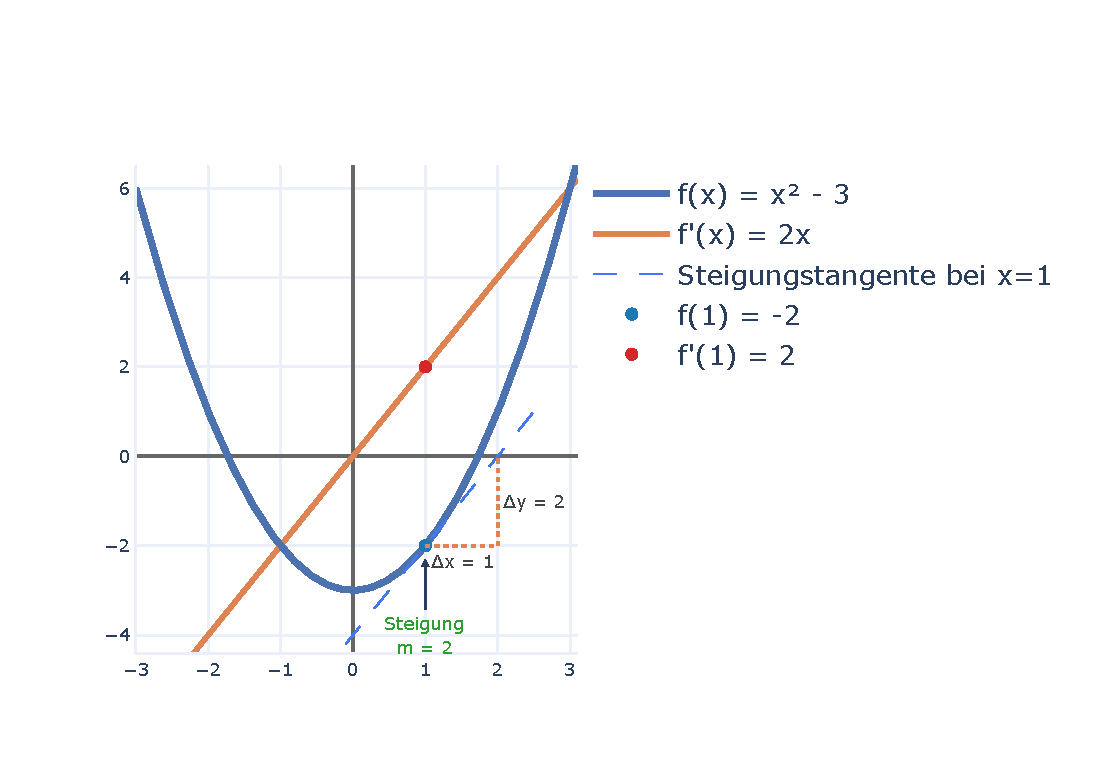
\includegraphics[width=0.85\linewidth]{./chapter2/media/NNGradientIntro.pdf}
	\caption[Understanding Gradients]{Understanding Gradients: The gradient of a 1D function $f(x)$ at point $x=1$ is calculated with the derivative $f'(x)$. It represents the slope of the tangent line at that point.}
	\label{fig:NNGradientIntro}
\end{figure}





\paragraph{Gradient Descent and Parameter Update} 
Gradient descent is an iterative optimization algorithm that is used to minimize a loss function~\cite{Bottou2016OptimizationMF}.
The basic principle of gradient descent can be understood by considering a simplified setting with a single parameter, which illustrates a network weight, see \autoref{fig:NNGradientDescent_2}. 
The horizontal axis represents the value of the weight, while the vertical axis represents the corresponding loss, which quantifies the discrepancy between the predicted and true values of the training data.

\begin{figure}[!h]
	\centering
	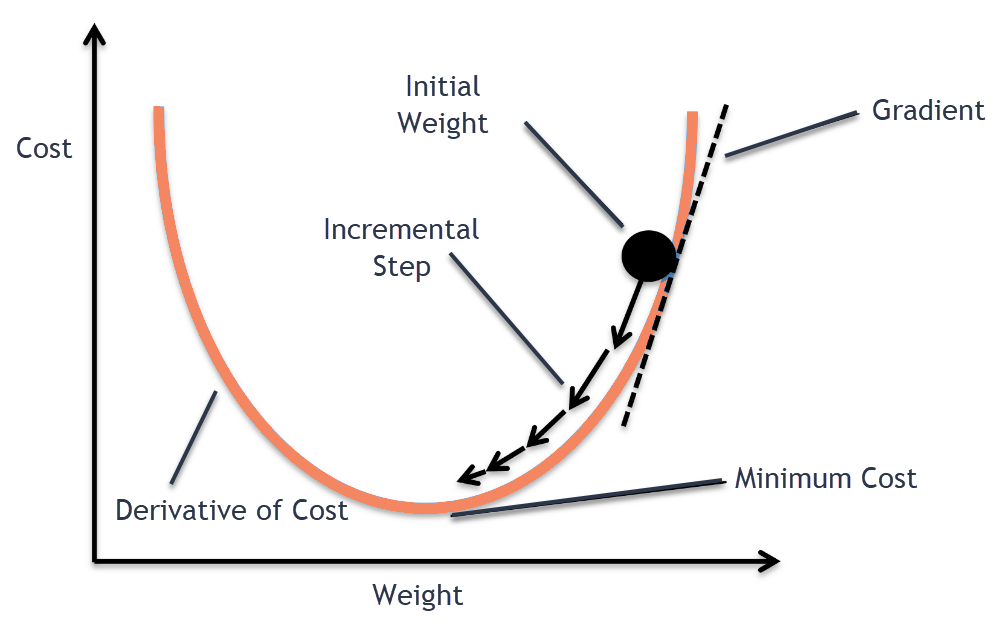
\includegraphics[width=0.6\linewidth]{./chapter2/media/NNGradientDescent_2}
	\caption[Neural Network: Simplified Gradient Descent]{Simplified gradient descent based on one network weight. Image source:~\cite{lanhamLearnARCoreFundamentals}.}
	\label{fig:NNGradientDescent_2}
\end{figure}

The resulting curve is the loss landscape for that one parameter. 
% At any point on the loss curve, the derivative (or gradient) indicates the local slope of the function.
% The current network weight, shown by the black dot must be updated in a way, to reduce the loss.
The current value of the weight, represented by the black dot, must be adjusted such that the loss decreases. Gradient descent achieves this through the following two steps:
\begin{enumerate}
	\item \textbf{Calculate the gradient:} 
	Compute the gradient of the loss function with respect to the weight. 
	% The gradient of the loss function with respect to the weight is calculated.
	% The first step is to compute the gradient of the loss function with respect to the weight. 
	The gradient indicates how the loss changes as the weight is adjusted.
	% The gradient of the loss function with respect to the parameter is calculated.
	\item \textbf{Update the weight:} The weight is then updated by moving in the opposite direction of the gradient. 
	Since the gradient points towards the direction of steepest increase, moving against it results in a reduction of the loss.
	% This is because the gradient points in the direction of steepest ascent, so moving in the opposite direction will lead to a decrease in the loss. 
	The basic parameter update is defined as:
	\begin{equation}	
		\mathbf{W}_{\text{t+1}} = \mathbf{W}_{\text{t}} - \alpha \cdot \nabla \mathcal{L}(\mathbf{W}_{\text{t}})
	\end{equation}
	where $\alpha$ denotes the learning rate, which controls the step size of the update and $\nabla \mathcal{L}(\mathbf{W}_{\text{t}})$ is the gradient of the loss function with respect to the parameter at iteration $t$.
	% where $\alpha$ is the learning rate, a hyperparameter that controls the step size of the update and $\nabla L(W_{\text{t}})$ is the gradient of the loss function with respect to the weight at its current value.	
\end{enumerate}


% In the example shown in Figure 2.5, the gradient is positive. Consequently, increasing the weight would increase the loss. To reduce the loss, the weight must therefore be moved in the opposite direction (to the left).
In the example shown in \autoref{fig:NNGradientDescent_2}, the gradient is positive. To reduce the loss, the weight must therefore be moved to the left, to the highest decrease of the function which is the negative gradient.
%  in the opposite direction (to the left). 
This procedure is repeated iteratively until the algorithm reaches a minimum of the loss function or another stopping criterion is satisfied. The successive parameter updates are illustrated by the black arrows in \autoref{fig:NNGradientDescent_2}. At the minimum, the gradient/the slope are zero and the parameter update becomes zero as well. The algorithm has converged. 
The goal is to find the optimal set of parameters that minimizes the loss function, which corresponds to the best fit of the model to the data, meaning the network's predictions are sufficiently accurate~\cite{Bottou2016OptimizationMF}. 




\paragraph{Optimization Problems}
Not every minimum found is a good solution. The loss landscape of neural networks is highly non-convex and can contain many local minima, saddle points and flat regions, where the gradient is zero but the loss is not minimized. If the gradient gets zero, the optimization process get stuck~\cite{Bottou2016OptimizationMF}. \autoref{fig:NNNetwork_OptimizationProblems} shows a loss landscape with two parameters. The black dot represents the inital parameter values and the line shows the trajectory of the parameter updates during training. As seen it depends on the initial parameter values, whether the algorithm converges to the global minima, local minama or to the saddle point in the middle of the two hills.  


\begin{figure}[!h]
	\centering
	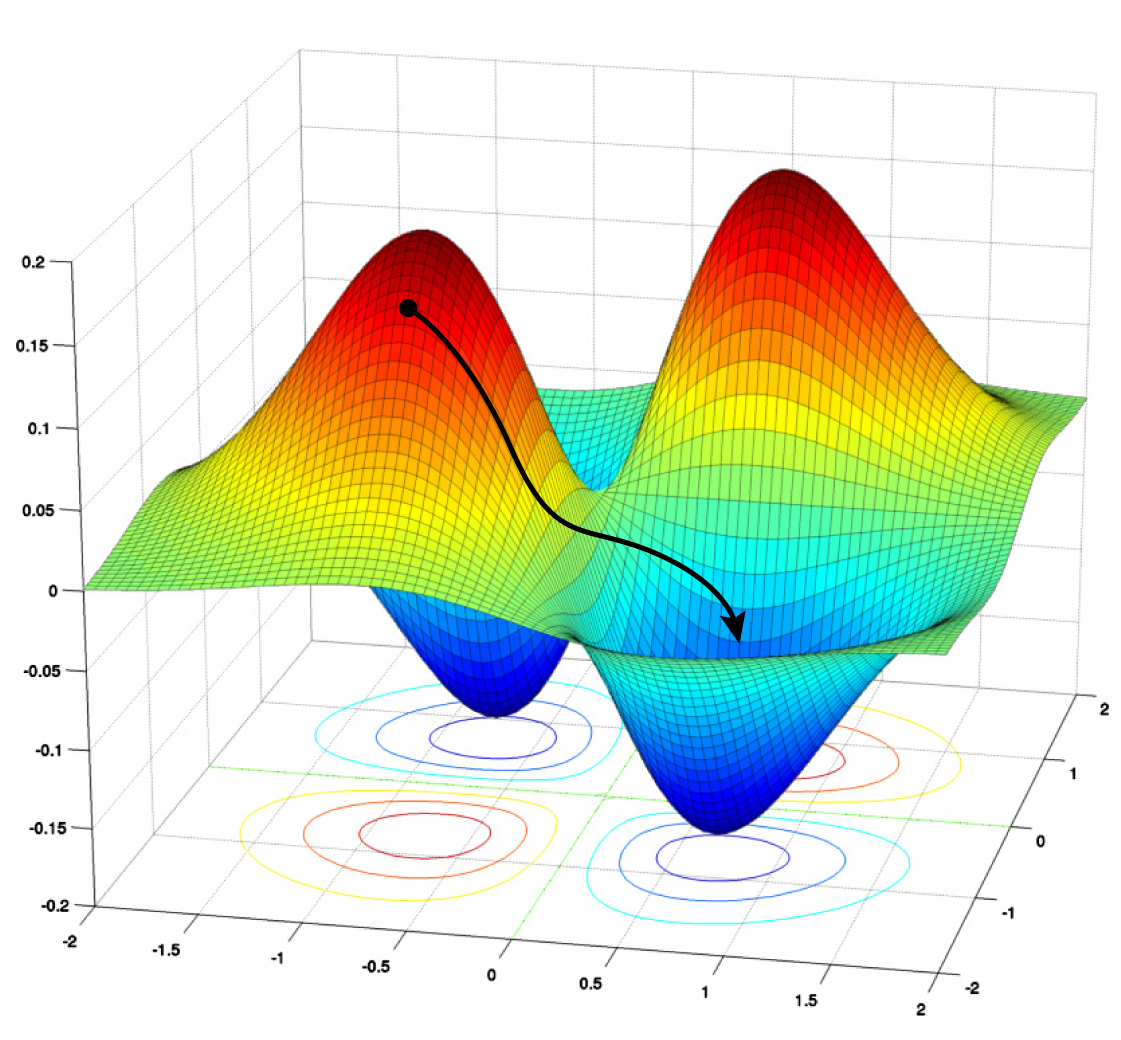
\includegraphics[width=0.5\linewidth]{./chapter2/media/NNGradientDescent}
	\caption[Neural Networks: Optimization Problems]{Neural Networks and their optimization Problems: The figure shows a loss landscape of two parameters, which has a local minima and a saddle point, where the training precess could get stuck. Image source:~\cite{ananthaswamyResearchersBuildAI2022}.}
	\label{fig:NNNetwork_OptimizationProblems}
\end{figure}

In the shown examples, the loss landscape was known, but in practice, the loss landscape of neural networks is typically unknown and can be highly complex.  Neural networks often consists of millions of parameters and therefore they have a high-dimensional loss landscape. The Algorithm works in such high-dimensional spaces in the same way.
% The optimization process works in such high-dimensional spaces in the same way and navigates through this loss landscape to find a set of parameters that minimizes the loss function. 
Therefore, training neural networks can be challenging and may require careful tuning of hyperparameters such as the learning rate, as well as the use of techniques like momentum, adaptive learning rates or regularization to improve convergence and generalization performance~\cite{Bottou2016OptimizationMF}. For this many variants of the basic gradient descent algorithm have been developed.


% \textit{Backpropagation.}
% The gradients needed for the parameter updates in gradient descent are computed using the backpropagation algorithm. Backpropagation efficiently propagates the error from the output layer back through the network to compute the necessary gradients for all parameters. For each neuron, the corresponding proportion of the total error is calculated and the weights are adjusted accordingly. 

\paragraph{Backpropagation}
The gradients required for updating the network parameters are computed using the backpropagation algorithm~\cite{Rumelhart1986LearningRB}. Backpropagation efficiently propagates the prediction error from the output layer back through the network and computes the gradients of the loss function $\mathcal{L}$ with respect to all weights $\mathbf{W}$ in the model. Based on these gradients, each parameter $w_{ij}^l$ is adjusted proportionally to its contribution to the overall error.
More precisely, backpropagation computes the partial derivatives of the loss function with respect to all trainable parameters in the network. These gradients quantify how sensitive the loss is to small changes in each parameter and therefore indicate how each parameter should be adjusted to reduce the overall error. Parameters that contribute more strongly to the error receive larger updates, while less influential parameters are adjusted more mildly.
The training process for a neural network can therefore be summarized by the following update rule:
\begin{equation}
\mathbf{W}_{t+1} = \mathbf{W}_t - \alpha \cdot \nabla_{\mathbf{W}_t} \left( \frac{1}{N} \sum_{i=1}^{N} \mathcal{L}\bigl(\mathbf{y}_i, f_{\mathbf{W}_t}(\mathbf{x}_i)\bigr) \right)
\end{equation}
where $f_{\mathbf{W}}$ denotes the neural network with parameters $\mathbf{W}$, $\mathcal{L}$ is the loss function measuring the difference between the predicted output $f_{\mathbf{W}}(\mathbf{x}_i)$ and the target value $\mathbf{y}_i$, $\alpha$ is the learning rate, $N$ is the number of training samples and $\nabla_{\mathbf{W}_t}$ represents the gradient of the loss function with respect to the weights at iteration $t$.
By iteratively applying this update rule, the network parameters are gradually adjusted in a direction that reduces the loss function and allows neural networks to reduce improve their predictions from training data.
% learn meaningful representations from training data
% . This iterative optimization process is what allows the neural network to learn meaningful representations from training data and improve its predictions over time.


Besides the standard gradient descent algorithm, which computes the gradient over the entire dataset, several more efficient variants are commonly used in practice. 
Instead of computing the gradient on the entire dataset, the variants stochastic and mini-batch gradient descent approximate it using one or a few training samples~\cite{Bottou2010LargeScaleML, Robbins1951ASA, Bottou2016OptimizationMF, Goodfellow-et-al-2016}, which reduces the computational cost per update while still providing a more stable gradient estimate compared to pure stochastic gradient descent.





\paragraph{Evaluation}
To measure the performance of a machine learning model, various evaluation metrics can be used depending on the specific task and problem setting. These metrics provide quantitative measures of how well a model performs and allow comparisons between different models or configurations. While common examples include accuracy, precision, recall and the F1-score for classification tasks, as well as mean squared error for regression tasks. However, a detailed discussion of these metrics is beyond the scope of this work.

The performance of a machine learning model is typically evaluated using data that has not been seen during training, referred to as test data. This allows an unbiased assessment of the model's ability to generalize to new, unseen samples. There exist in general three main scenarios regarding the model's performance on training and test data:
\begin{itemize}
	\item \textbf{Underfitting:} A model that underfits performs poorly on both training and test data. It fails to capture the underlying patterns in the training data, resulting in high error on both datasets.
	\item \textbf{Overfitting:} An overfitted model achieves high performance on the training data but fails to generalize well to the test data. It has essentially memorized the training samples, including noise and outliers, which leads to poor performance on new data.
	\item \textbf{Well-Balanced Model:} A well-balanced model achieves consistently good performance on both training and test datasets. It captures the underlying patterns in the training data without overfitting, allowing it to generalize effectively to unseen samples. 
\end{itemize}






\section{Convolutional Neural Networks}

A Convolutional Neural Network (CNN) is a deep neural network architecture designed to process grid-like data, especially images~\cite{LeCun1998GradientbasedLA, Krizhevsky2012ImageNetCW}. CNNs are particularly effective for visual tasks because they exploit the spatial structure of an image and learn local patterns such as edges, corners and textures. Unlike fully connected networks, CNNs do not treat every pixel independently. Instead, they use small learnable filters that are applied across the image to detect relevant structures at different positions~\cite{Khan2025ACS, Younesi2024ACS, Long2022}.

\paragraph{Convolution}

The main idea of a CNN is the convolution operation, where a filter, also known as kernel, is applied to the image to extract features. For example, the Prewitt kernels, also known as edge detection filters, can be used to detect horizontal and vertical edges in an image:
\begin{equation}
	K_{\text{horizontal}} =
	\begin{bmatrix}
		-1 & 0 & 1\\
		-1 & 0 & 1\\
		-1 & 0 & 1
	\end{bmatrix}
	\qquad
	K_{\text{vertical}} =
	\begin{bmatrix}
		-1 & -1 & -1\\
		0 & 0 & 0\\
		1 & 1 & 1
	\end{bmatrix}
\end{equation}

\autoref{fig:CNNCatPrewitt} shows the result, after applying the Prewitt kernels to a grey-scale image. There exists a wide variety of predefined filters to extract various of visual structures from the image. 
\begin{figure}[h]
    \centering
    \subfigure[Original Image: No convolution is applied]{
        \parbox{4.6cm}{
            \centering
            {\small\textbf{Original}}\par
            \vspace{0.3em}
            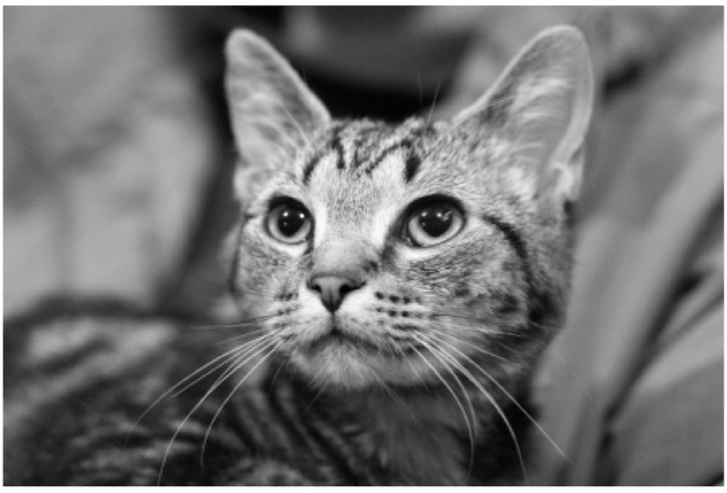
\includegraphics[width=4.5cm]{./chapter2/media/CNNCatPrewittOriginal_3}
        }
        \label{fig:CNNCatPrewittOriginal}
    }
    \hspace{0.3cm}
    \subfigure[Convolved Image, after the horizontal Prewitt kernel is applied to the original image]{
        \parbox{4.7cm}{
            \centering
            {\small\textbf{Horizontal Prewitt}}\par
            \vspace{0.3em}
            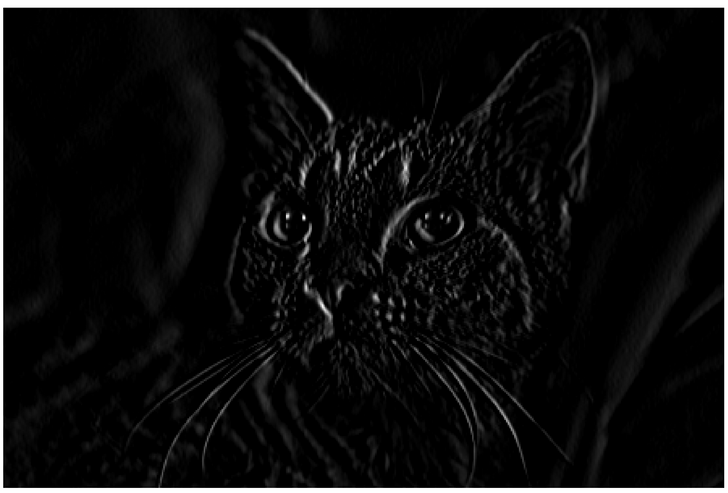
\includegraphics[width=4.5cm]{./chapter2/media/CNNCatPrewittHorizontal_3}
        }
        \label{fig:CNNCatPrewittHorizontal}
    }
    \hspace{0.3cm}
    \subfigure[Convolved Image, after the vertical Prewitt kernel is applied to the original image]{
        \parbox{4.6cm}{
            \centering
            {\small\textbf{Vertical Prewitt}}\par
            \vspace{0.3em}
            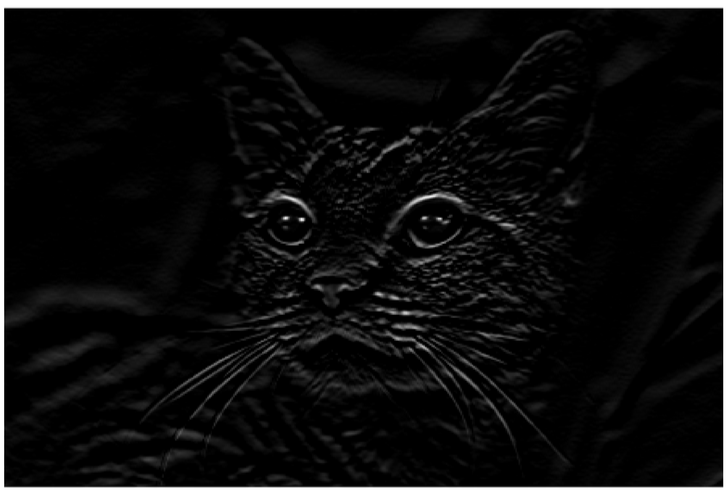
\includegraphics[width=4.5cm]{./chapter2/media/CNNCatPrewittVertical_3}
        }
        \label{fig:CNNCatPrewittVertical}
    }
    \caption[CNN: Convolution of a Greyscale Image using Prewitt Kernels]{Convolution of a greyscale image using Prewitt kernels. Image sources:~\cite{UnderstandingFiltersConvolutional}.}
    \label{fig:CNNCatPrewitt}
\end{figure}




A Filter or kernel is defined as a small matrix of weights, is moved across the image and element-wise multiplied with the underlying pixel values~\cite{Dumoulin2016AGT, Khan2025ACS, Younesi2024ACS, Long2022}. This is possible, because an image is technically a matrix of pixel values too. The resulting values are stored in a new matrix called a feature map, which highlights the patterns detected by the kernel. Since the same kernel is reused at every pixel location, CNNs are able to detect the same feature independent of its position in the image.
% Figure \autoref{fig:CNNConvolutionIntro} illustrates the mathematical convolution operation, where a $3 \times 3$ kernel is applied to a $6 \times 6$ image. The results are stored in a $3 \times 3$ matrix. 

During the convolution process, a kernel (dark blue) slides across the image (light blue), and at each position the element-wise products are summed to generate a single output value that is stored in the feature map (olive green), as shown in \autoref{fig:CNNConvolution_1}.
Figure~\ref{fig:CNNConvolutionIntro} illustrates the mathematical convolution operation, where a $3 \times 3$ kernel is applied to a $6 \times 6$ image to produce a $3 \times 3$ output matrix. 
\begin{figure}[!h]
	\centering
	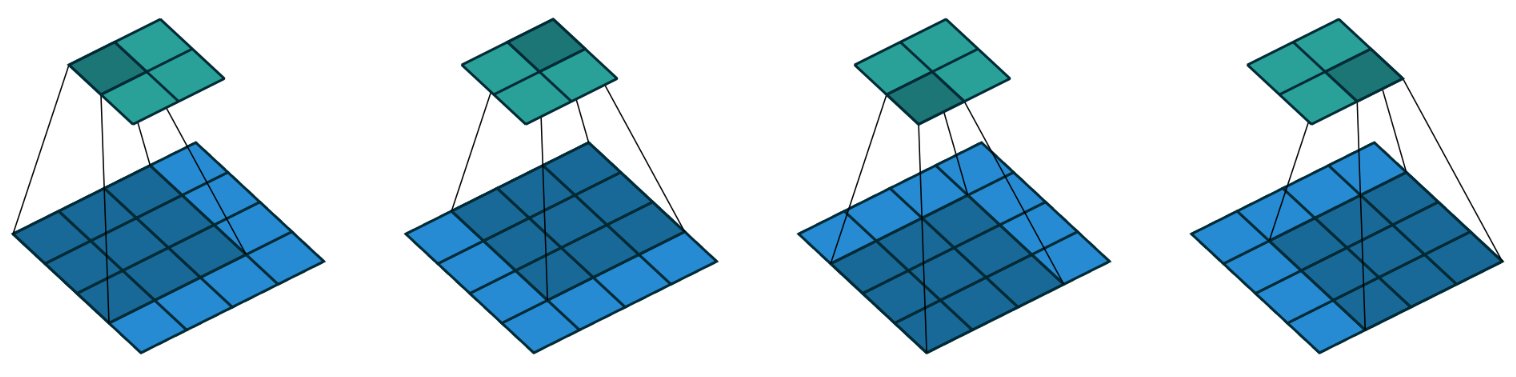
\includegraphics[width=0.75\linewidth]{./chapter2/media/CNNConvolution_1.png}
	\caption[CNN Convolution: Convolution of an Image with the Resulting Feature Map]{Convolution of an image with the resulting feature map. Image source:~\cite{Dumoulin2016AGT}.}
	\label{fig:CNNConvolution_1}
\end{figure}

\begin{figure}[!h]
	\centering
	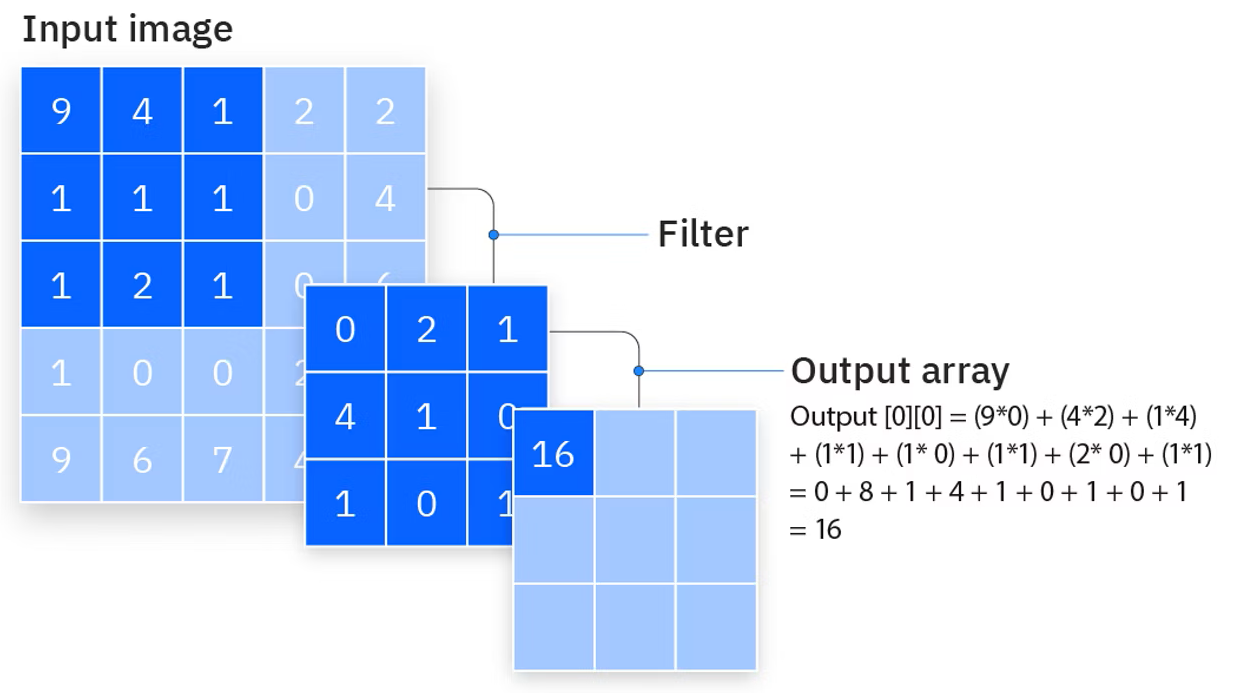
\includegraphics[width=0.65\linewidth]{./chapter2/media/CNNConvolutionIntro.png}
	\caption[CNN Convolution: Mathematical concept]{Mathematical concept of the convolution in \acsp{CNN} using element-wise multiplication. Image source:~\cite{WhatAreConvolutional2021}.}
	\label{fig:CNNConvolutionIntro}
\end{figure}

% Figure \autoref{fig:CNNConvolution_1} shows how the kernel (dark blue) is slided across the image (light blue) step by step. At each location the element-wise products are summed up to obtain one output value, which is stored in a feature map (olive green). 

A CNN consist of multiple kernels, which are applied in parallel and in multiple layers to the image, resulting in multiple feature maps. Importantly, in a CNN the kernels are not fixed manually, instead they are learned during training, allowing the network to find the optimal filters for the task success~\cite{Khan2025ACS, Younesi2024ACS, Long2022}.


% Figures \autoref{fig:CNNConvolutionIntro_View2} shows an alternative view of the convolution process.
% \begin{figure}[!h]
% 	\centering
% 	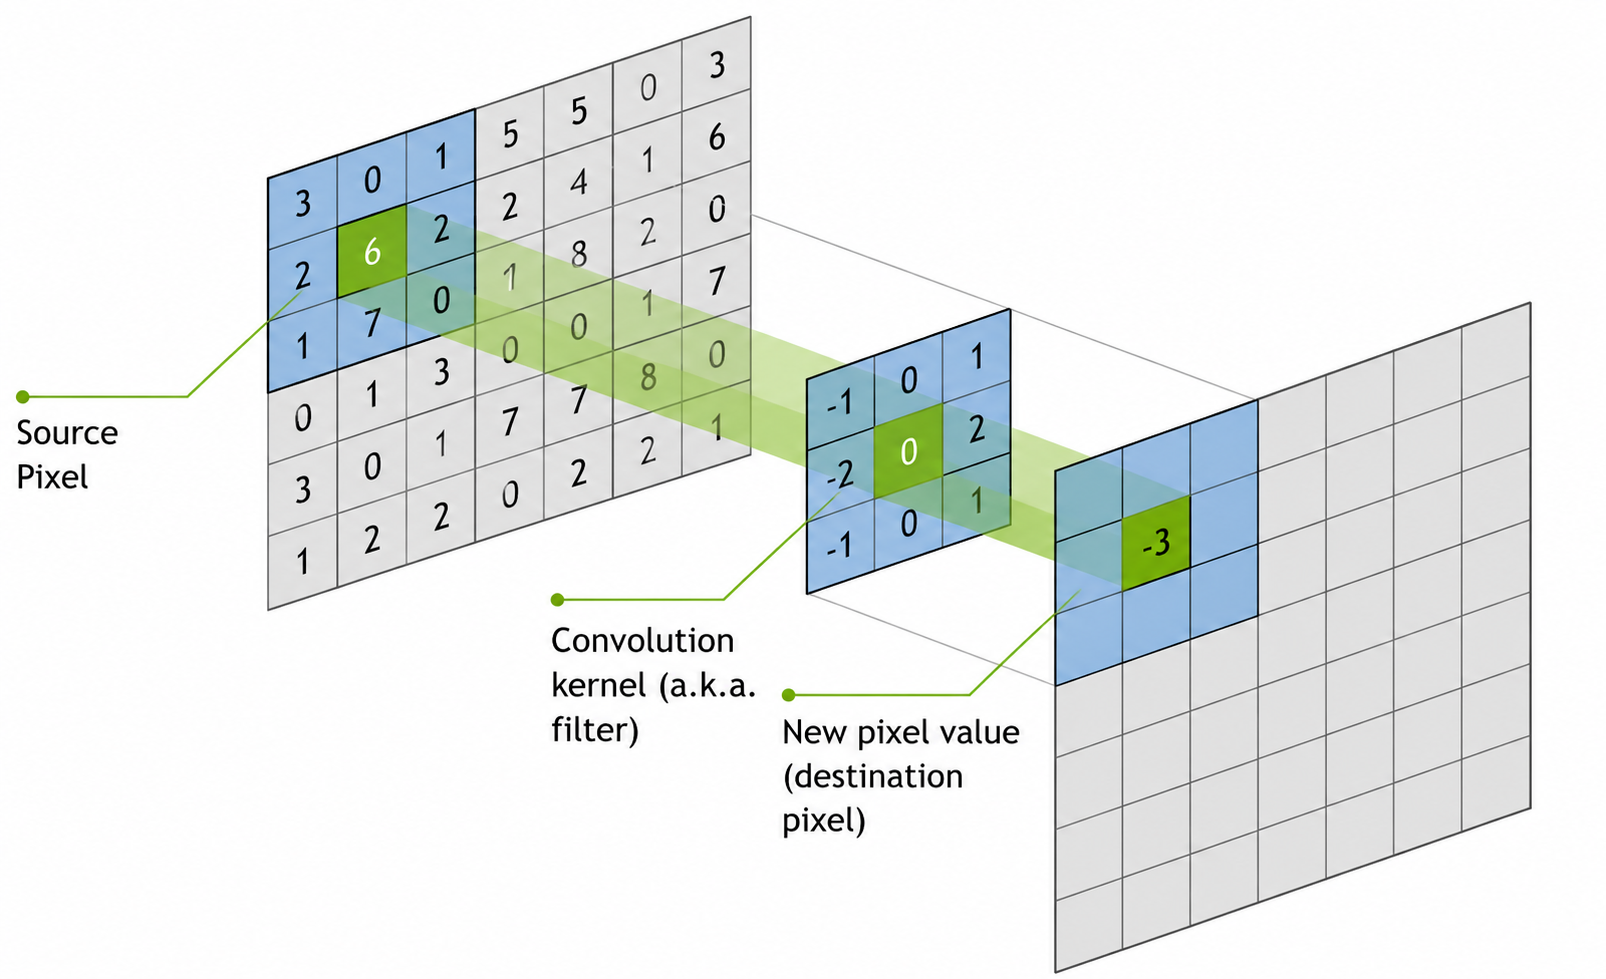
\includegraphics[width=0.65\linewidth]{./chapter2/media/CNNConvolutionIntro_View2.png}
% 	\caption[CNN Convolution Introduction]{CNN Convolution Introduction. Image adapted from:~\cite{WhatConvolutionalNeural}.}
% 	\label{fig:CNNConvolutionIntro_View2}
% \end{figure}


\paragraph{Padding}
As seen in the Figures \ref{fig:CNNConvolutionIntro} and \ref{fig:CNNConvolution_1}, the feature map is smaller than the original image, because of the convolution operation. 
To preserve the spatial resolution of the input image, padding is often added around the border before applying the convolution, see \autoref{fig:CNNConvolution_1_withPadding}~\cite{Dumoulin2016AGT, Khan2025ACS, Younesi2024ACS, Long2022}. With zero-padding, the image size can remain unchanged after the convolution, which is useful when multiple convolution layers are stacked. 
\begin{figure}[!h]
	\centering
	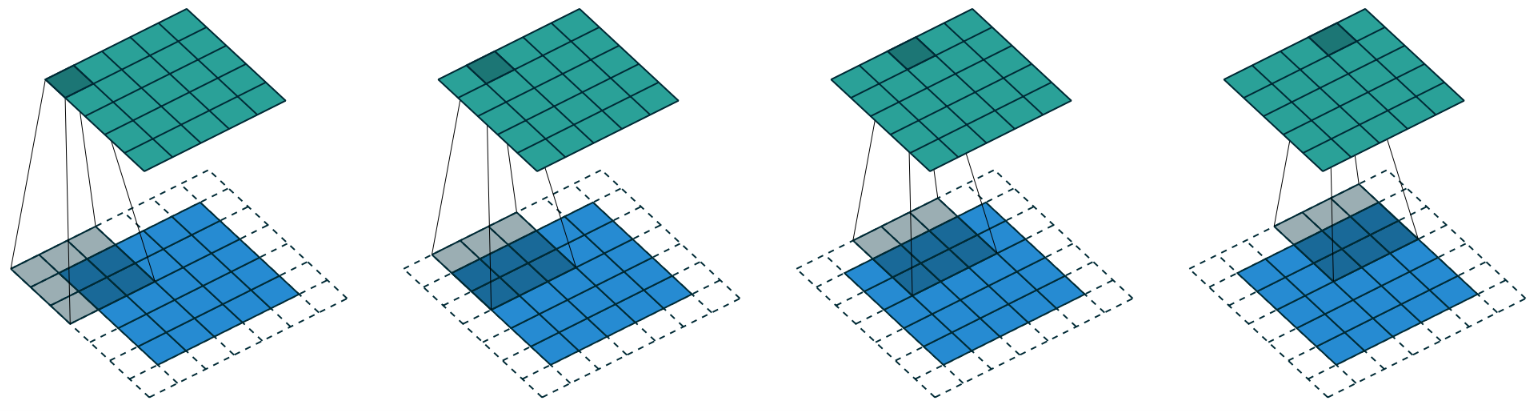
\includegraphics[width=0.75\linewidth]{./chapter2/media/CNNConvolution_1_withPadding}
	\caption[CNN Convolution with Padding]{CNN Convolution with Padding. Image source:~\cite{Dumoulin2016AGT}.}
	\label{fig:CNNConvolution_1_withPadding}
\end{figure}





\paragraph{Activation Function}
After the convolution operation, a non-linear activation function is applied to the resulting feature map~\cite{Khan2025ACS, Younesi2024ACS, Long2022}. Activation functions introduce non-linearity into the network, allowing CNNs to learn complex visual patterns that cannot be represented by linear transformations alone~\cite{Hanin2017ApproximatingCF}.
The most commonly used activation function is ReLU~\cite{Khan2025ACS, Hanin2017ApproximatingCF, Long2022}:
which replaces all negative values with zero while leaving positive values unchanged:
\begin{equation}
	f(x)=\max(0,x)
\end{equation}
By applying the ReLU function after each convolution, the network can learn increasingly complex feature representations across multiple layers.


\paragraph{Pooling Layer}
Another central component of CNNs is the pooling layer~\cite{Khan2025ACS, Long2022}. Pooling reduces the spatial size of the feature maps while retaining the most important information. This lowers the computational cost and increases robustness to small shifts in the input image.
A common choice is a $2\times2$ pooling window with a stride of 2. In this case, the feature map is divided into non-overlapping $2\times2$ regions and each region is summarized by a single value~\cite{Younesi2024ACS, Khan2025ACS}. As a result, the width and height of the feature map are reduced by a factor of two.

Two common pooling methods are max pooling and average pooling~\cite{Younesi2024ACS, Khan2025ACS}, as illustrated in \autoref{fig:CNNPooling}. In max pooling, the largest value within each pooling region is selected and propagated to the output feature map. In average pooling, the mean value of all elements within the region is computed. Both methods reduce the spatial resolution while preserving the most relevant information contained in the feature map.
Pooling layers are typically applied after convolution layers and allow the network to build increasingly compact feature representations. While early convolution layers extract local patterns such as edges and textures, pooling helps summarize these features and enables deeper layers to focus on higher-level visual structures~\cite{Younesi2024ACS, Khan2025ACS, Long2022}.

\begin{figure}[!h]
	\centering
	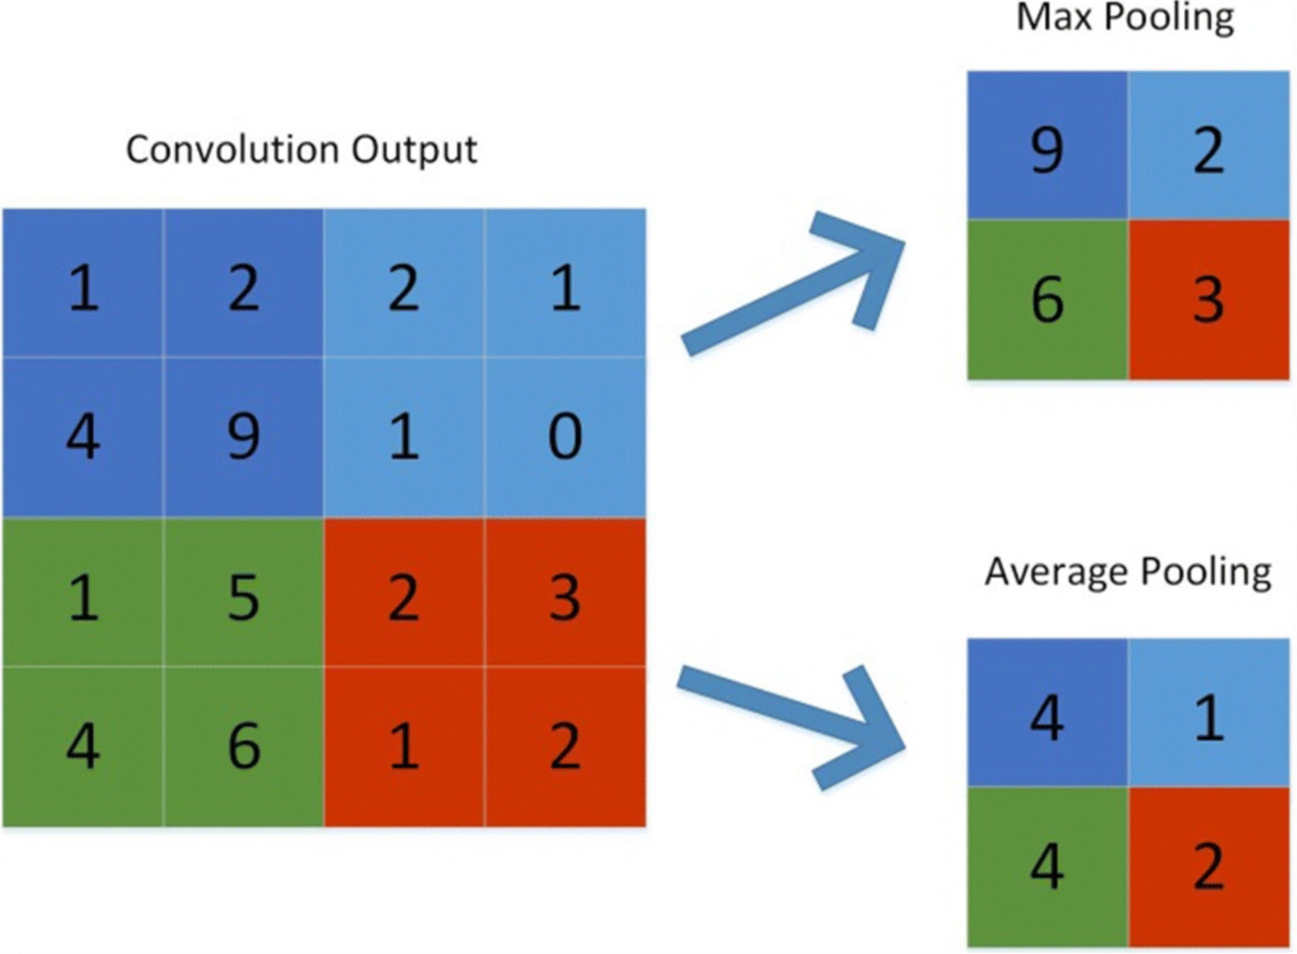
\includegraphics[width=0.4\linewidth]{./chapter2/media/CNNPooling}
	\caption[CNN Pooling]{CNN Pooling: Illustration of max pooling and average pooling operations with a stride of 2. Image source:~\cite{jiangEightlayerConvolutionalNeural2020}.}
	\label{fig:CNNPooling}
\end{figure}
% \begin{figure}[!h]
% 	\centering
% 	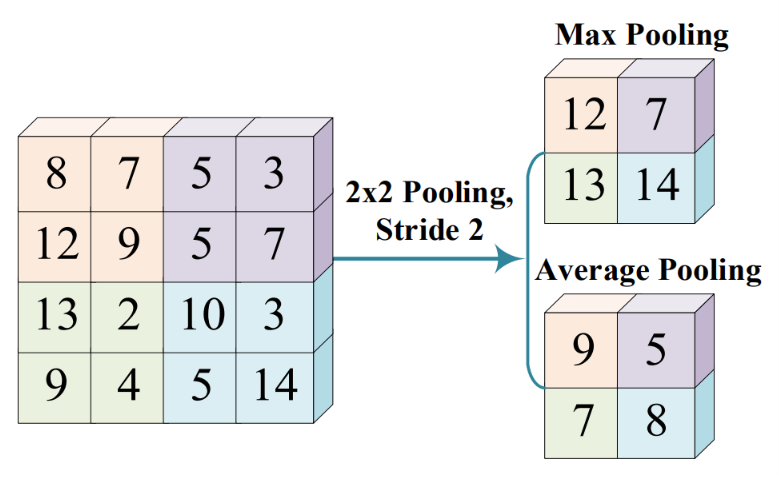
\includegraphics[width=0.45\linewidth]{./chapter2/media/CNNPooling_2.png}
% 	\caption[CNN Pooling]{CNN Pooling. Image source:~\cite{Khan2025ACS}.}
% 	\label{fig:CNNPooling}
% \end{figure}


\paragraph{CNN Pipeline}

The common CNN processing sequence is: convolution, activation function and pooling, while the activation function is often not mentioned explicitly.
A CNN usually consists of several repeated blocks of convolution and pooling layers. Early layers detect simple features such as edges and corners, while deeper layers combine these basic features into more complex structures. 
After several convolution and pooling stages, the feature maps are flattened into one big vector and passed through a MLP or a classification head in a classification task to produce the final predictions, see \autoref{fig:CNNPipeline}. Through backprobagating the prediction error, the networks parameter are adjusted during training.

\begin{figure}
	\centering
	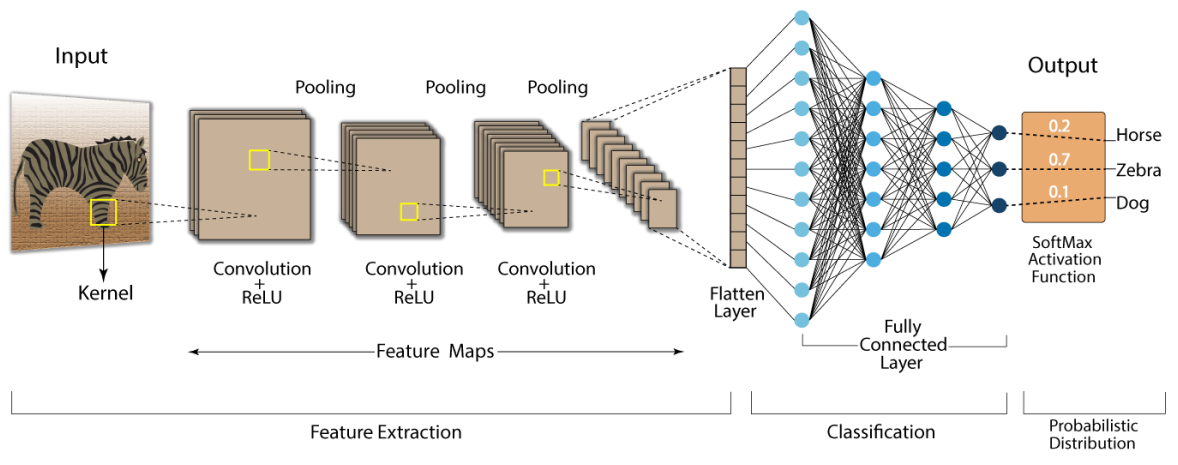
\includegraphics[width=1.0\linewidth]{./chapter2/media/CNNPipeline.png}
	\caption[CNN Pipeline]{CNN Pipeline: Illustration of the typical processing sequence in a CNN, including convolution, activation function, and pooling layers. Image source:~\cite{swapnaConvolutionalNeuralNetwork2020}.}
	\label{fig:CNNPipeline}
\end{figure}



\paragraph{RGB Images}
The same principle can be extended to RGB images~\cite{Khan2025ACS, Long2022, Krizhevsky2012ImageNetCW}. While a grayscale image contains only a single channel, an RGB image consists of three color channels representing red, green and blue values. Consequently, a convolution kernel must span all input channels. For a kernel size of $3\times3$, a common way is to use an $3\times3\times3$ kernel for an RGB image~\cite{Khan2025ACS, Long2022, Krizhevsky2012ImageNetCW}. This kernel is applied across all three color channels simultaneously and the resulting values are summed up to produce a single output value in the feature map. By learning appropriate kernels during training, CNNs can effectively capture complex visual patterns across all color channels in RGB images.
% The resulting values are summed to produce a single output value in the feature map.
%  The same idea can be extended to RGB images, where the kernels operate across all color channels.









\section{Transformer}
% for sequence-to-sequence tasks
A Transformer is a deep neural network architecture designed to process sequential data, especially text~\cite{Vaswani2017AttentionIA}. It's the foundation for most modern LLMs, enabling them to process and understand language effectively.
Unlike earlier architectures that process tokens sequentially, Transformers compare all tokens in a sequence in parallel and learn which parts of the input are most relevant to each other. This is archieved through the attention mechanism, the core innovation of the Transformer architecture~\cite{Vaswani2017AttentionIA, AttentionTransformersStepbystep, TransformerExplainerLLM, Raschka2024BuildLLM}. 
Rather than treating all tokens equally, the model assigns greater importance to contextually relevant tokens, allowing it to capture long-range dependencies in a sentence and are crucial for language understanding
% The main idea is simple: when the model reads one token, it does not treat all other tokens equally. It assigns higher importance to the tokens that are more relevant in the current context. This makes Transformers especially powerful for language tasks, because meaning often depends on long-range dependencies in the sentence.

% \paragraph{Architecture Overview}
The original Transformer architecture was introduced by \textcite{Vaswani2017AttentionIA} and consists of two parts: the encoder and the decoder. See \autoref{fig:TransformerArchitecture} for an overview.
\begin{enumerate}
	\item \textbf{Encoder:} The encoder reads the full input sequence and converts it into a contextual latent representation. Each token is transformed not only based on its own identity, but also based on the other tokens in the sequence. In this way, the encoder builds a rich internal representation of the input.
	
	\item \textbf{Decoder:} The decoder generates the output sequence autoregressively, meaning one token at a time. To produce the next token in the output sequence, it uses at each prediction step: (1) The contextual representation from the encoder. (2) The previously generated output tokens from the decoder. This allows the decoder to produce the next token while taking the source sequence into account.
\end{enumerate}


\begin{figure}[!t]
	\centering
	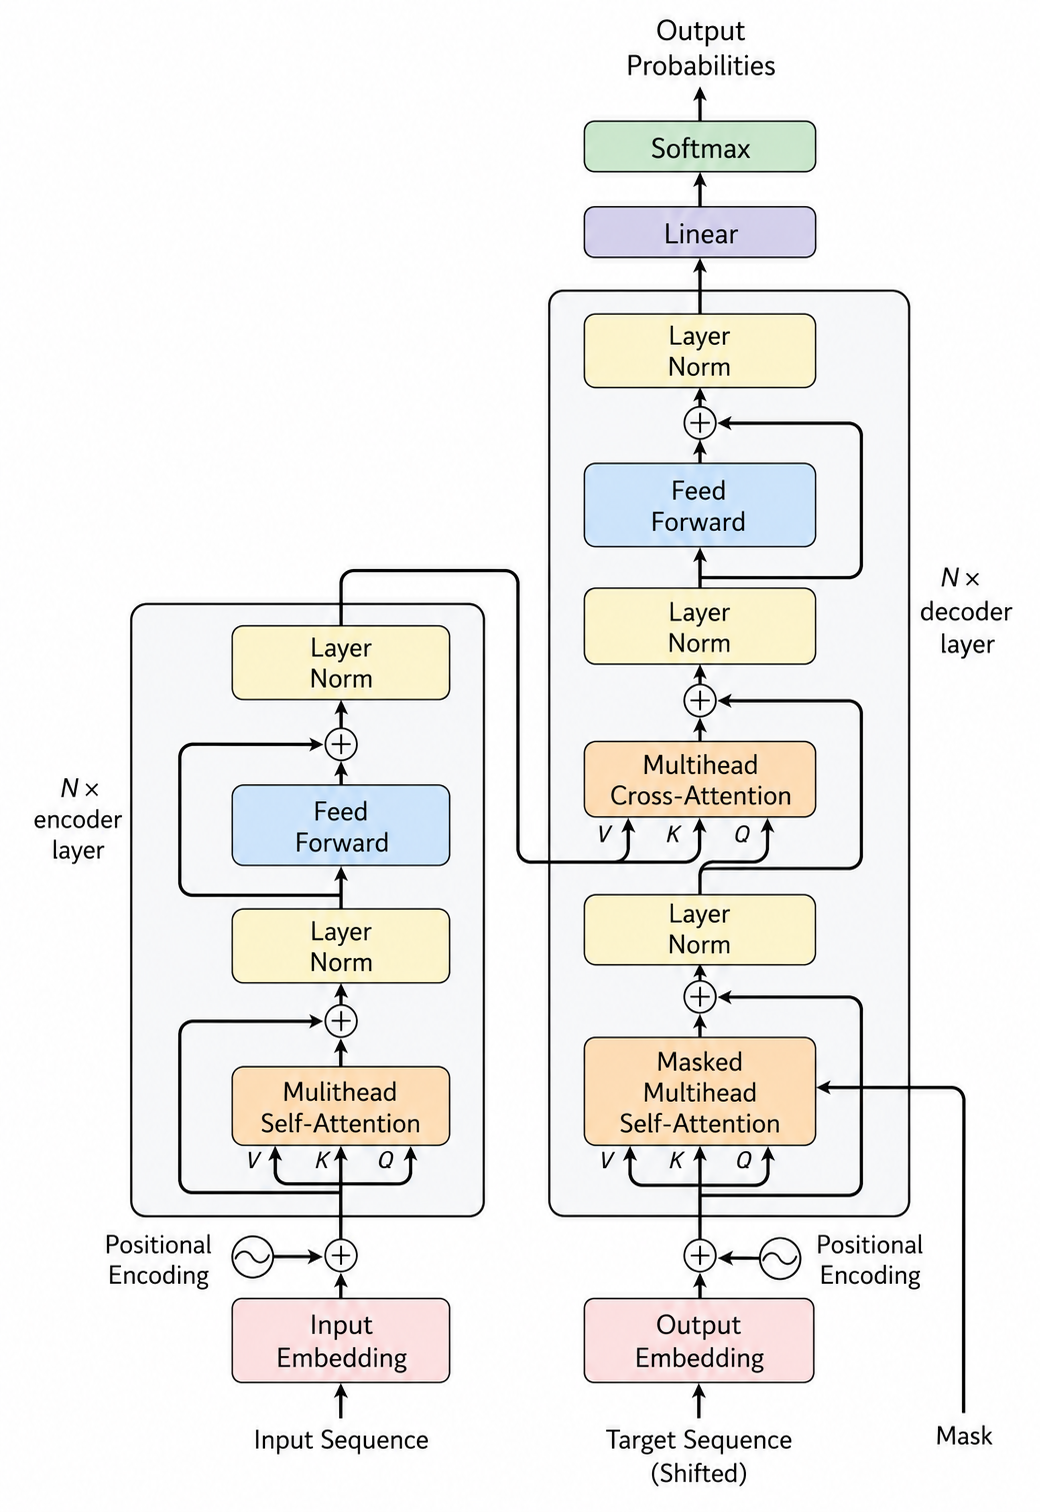
\includegraphics[width=0.6\linewidth]{./chapter2/media/TransformerArchitectur3}
	\caption[Transformer Architecture]{Original Transformer architecture, consisting of an encoder and a decoder part. Image based on:~\cite{Vaswani2017AttentionIA}.}
	\label{fig:TransformerArchitecture}
\end{figure}

While the examples in this section are based on text processing to facilitate understanding of the Transformer architecture, the underlying principles generalize to other modalities, such as images or videos. 



\paragraph{Input Embeddings}
Before a Transformer can process data, the data must be converted into vectors, which is done by the input embedding layer~\cite{Raschka2024BuildLLM}.  Given an input text such as ``Data visualization empowers users to'', the model first tokenizes the text, then maps each token to a vector representation and finally adds positional information~\cite{Raschka2024BuildLLM, TransformerExplainerLLM}. The resulting embedding combines semantic meaning with information about token order. 
\begin{enumerate}
	\item \textbf{Tokenization:} The input text is split into smaller units called tokens. These tokens can be a word, a subword or a single character. For example, the sentence might be tokenized into ["Data", "visualization", "empowers", "users", "to"]. Each token is assigned a unique token ID.
	\item \textbf{Embedding:} Each token is then mapped one-to-one to a high-dimensional vector representation. This embedding captures the semantic meaning of the token. For example, the token "Data" might be represented as a 768-dimensional vector in the embedding space.
	\item \textbf{Positional Encoding:} Since the Transformer does not process tokens sequentially, it needs an explicit way to represent token order. Positional encodings provide this information. Depending on the model, these encodings may be fixed or learned. They are added to the token embeddings so that the model can distinguish between, for example, ``dog bites man'' and ``man bites dog''.
	\item \textbf{Final Embedding:} The final input representation is obtained by combining token embeddings and positional information, typically through element-wise addition. This representation is then passed into the Transformer layers.
\end{enumerate}


\paragraph{Attention Mechanism}
The Attention mechanism is responsible for capturing contextual relationships between tokens by directly computing their relevance to one another. This allows the model to understand long-range dependencies and contextual relationships of the tokens, leading to more coherent and relevant output~\cite{Raschka2024BuildLLM, TransformerExplainerLLM, AttentionTransformersStepbystep}. 
In \autoref{fig:TransformerAttentionWeights} the attention weights of the word ``it'' in the sentence ``The animal didn't cross the street because it was too tired'' are visualized, after the input is processed through the Encoder attention mechanism. The attention weights allows the model to decide which other tokens in the sequence are most relevant. 
% The attention mechanism allows the model to determine that ``it'' refers to ``The animal'' and not to ``the street'' and simultaneously it refers to the context ``too tired'', which is crucial for understanding the meaning of the sentence. 

\begin{figure}
	\centering
	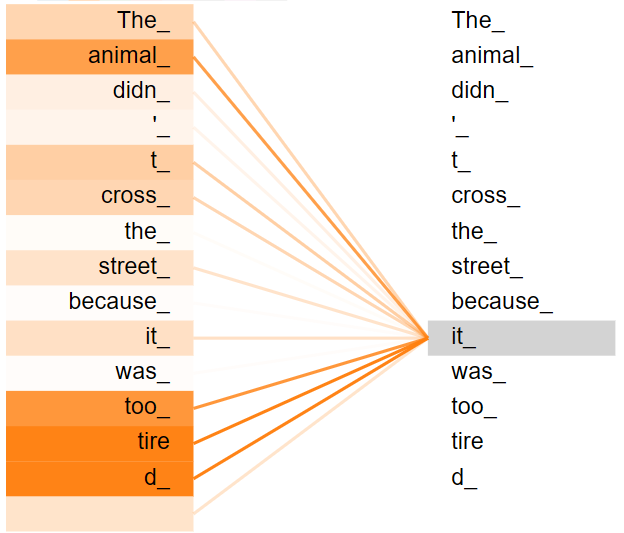
\includegraphics[width=0.4\linewidth]{./chapter2/media/AttentionWords2}
	\caption[Transformer: Attention Weights Example]{Attention Weights of the word ``it'' in a sentence. Image source:~\cite{GoogleColab}}
	% https://colab.research.google.com/github/tensorflow/tensor2tensor/blob/master/tensor2tensor/notebooks/hello_t2t.ipynb#scrollTo=OJKU36QAfqOC.
	\label{fig:TransformerAttentionWeights}
\end{figure}

\textit{Compute Attention Weights.} In the self-attention mechanism, each token embedding vector $\mathbf{x}^{(i)}$ is transformed into three different representations: query $\mathbf{q}^{(i)}$, key $\mathbf{k}^{(i)}$ and value $\mathbf{v}^{(i)}$. These representations are obtained through learnable linear transformations with parameters ($W_q$, $W_k$, $W_v$) that are optimized during training~\cite{Raschka2024BuildLLM, TransformerExplainerLLM, AttentionTransformersStepbystep}.
\begin{itemize}
	\item \textbf{Query $\mathbf{q}^{(i)}=\mathbf{x}^{(i)}\mathbf{W}_q$:} The query vector represents the token for which attention is computed. It is used to determine how much attention this token should pay to other tokens in the sequence.
	\item \textbf{Key $\mathbf{k}^{(i)}=\mathbf{x}^{(i)}\mathbf{W}_k$:} The key vector represents the token against which the query is compared. It is used to compute the relevance score between the query and the token.
	\item \textbf{Value $\mathbf{v}^{(i)}=\mathbf{x}^{(i)}\mathbf{W}_v$:} The value vector contains the actual information of the token. It is weighted by the attention scores to produce the final output of the self-attention mechanism.
\end{itemize}


\textit{Single-Head Self-Attention.}
% \textit{Self-Attention.} 
The query vectors are then compared with the key vectors of all tokens in the sequence using the dot product (scalar product), producing relevance scores that indicate how strongly tokens are related to one another. To stabilize training, these scores are scaled by the square root of the key dimension $d_k$ and normalized using a softmax function, resulting in attention weights. Finally, the attention weights are applied to the corresponding value vectors $\mathbf{v}^{(i)}$ and these weighted values are aggregated to produce the new context vector $\mathbf{z}^{(i)}$ and the output of the self-attention layer~\cite{Raschka2024BuildLLM, TransformerExplainerLLM, AttentionTransformersStepbystep}, see \autoref{fig:TransformerAttentionKeyQueryValueSimply}. 
\begin{equation}
	\mathbf{z}^{(i)} = \text{softmax}\left(\frac{\mathbf{q}^{(i)} \cdot \mathbf{k}^{(i)T}}{\sqrt{d_k}}\right) \cdot \mathbf{v}^{(i)}
\end{equation}
In this way, each token can incorporate information from the most relevant tokens in the sequence, enabling the model to capture contextual dependencies. 
But what does this mean technically? The value vector $\mathbf{v}^{(i)}$ represents the token's information in a semantically learned high-dimensional embedding space. Through the attention mechanism, the vector's direction and magnitude in this embedding space are adjusted, resulting in a different semantic meaning.
In \autoref{fig:TransformerEmbeddingSpace_BlueFluffyCreature4}, it is shown how the vector of the word ``creature'' is shifted in the embedding space based on the context ``a fluffy blue creature''. This illustrates how the attention mechanism allows the model to dynamically adjust the meaning of tokens based on their relationships with other tokens in the sequence~\cite{AttentionTransformersStepbystep}.
% In one context, it may point to a specific type of creature, while in another context, it may point to a different type of creature.
% According to the relevant semantic meaning, the word “creature” is affected within the vectorial embedding space by the words (embeddings) “fluffy” and “blue”
\begin{figure}[!h]
	\centering
	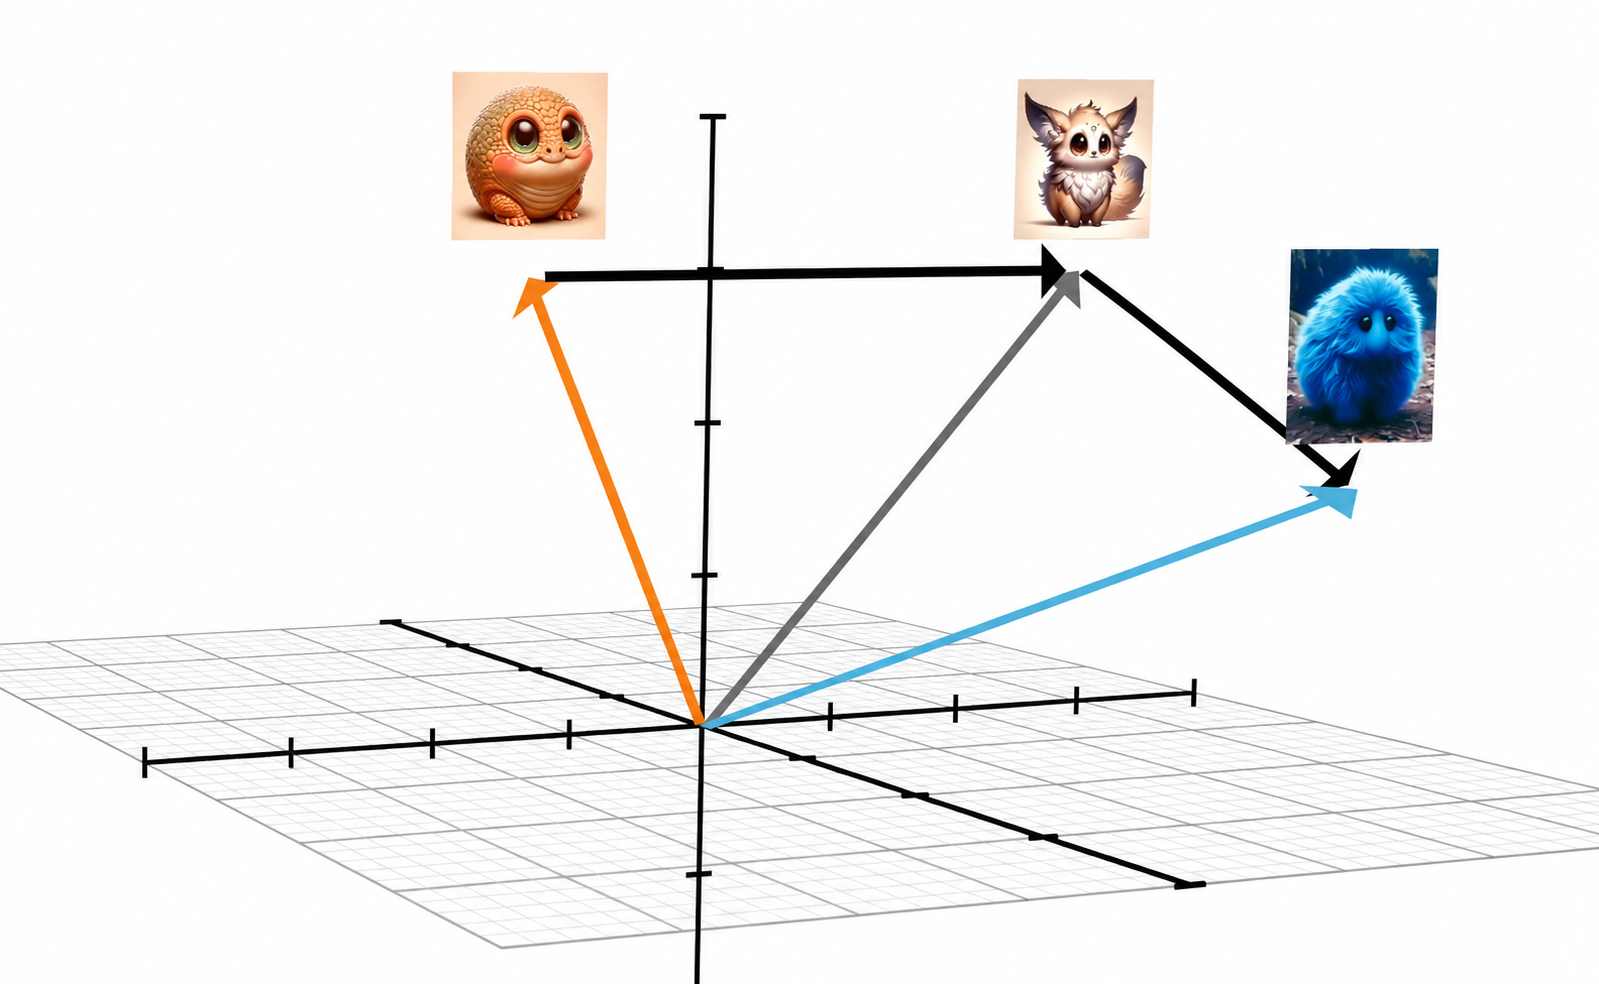
\includegraphics[width=0.6\linewidth]{./chapter2/media/TransformerEmbeddingSpace_BlueFluffyCreature4}
	\caption[Transformer: Embedding Space]{Illustration of the value embedding space $V$: The vector of ``creature'' is shifted in the embedding space based on the context ``a fluffy blue creature''. Image source:~\cite{AttentionTransformersStepbystep}.}
	\label{fig:TransformerEmbeddingSpace_BlueFluffyCreature4}
\end{figure}
% are weighted by the attention scores, allowing each token to aggregate information from other tokens based on their relevance.

\begin{figure}
	\centering
	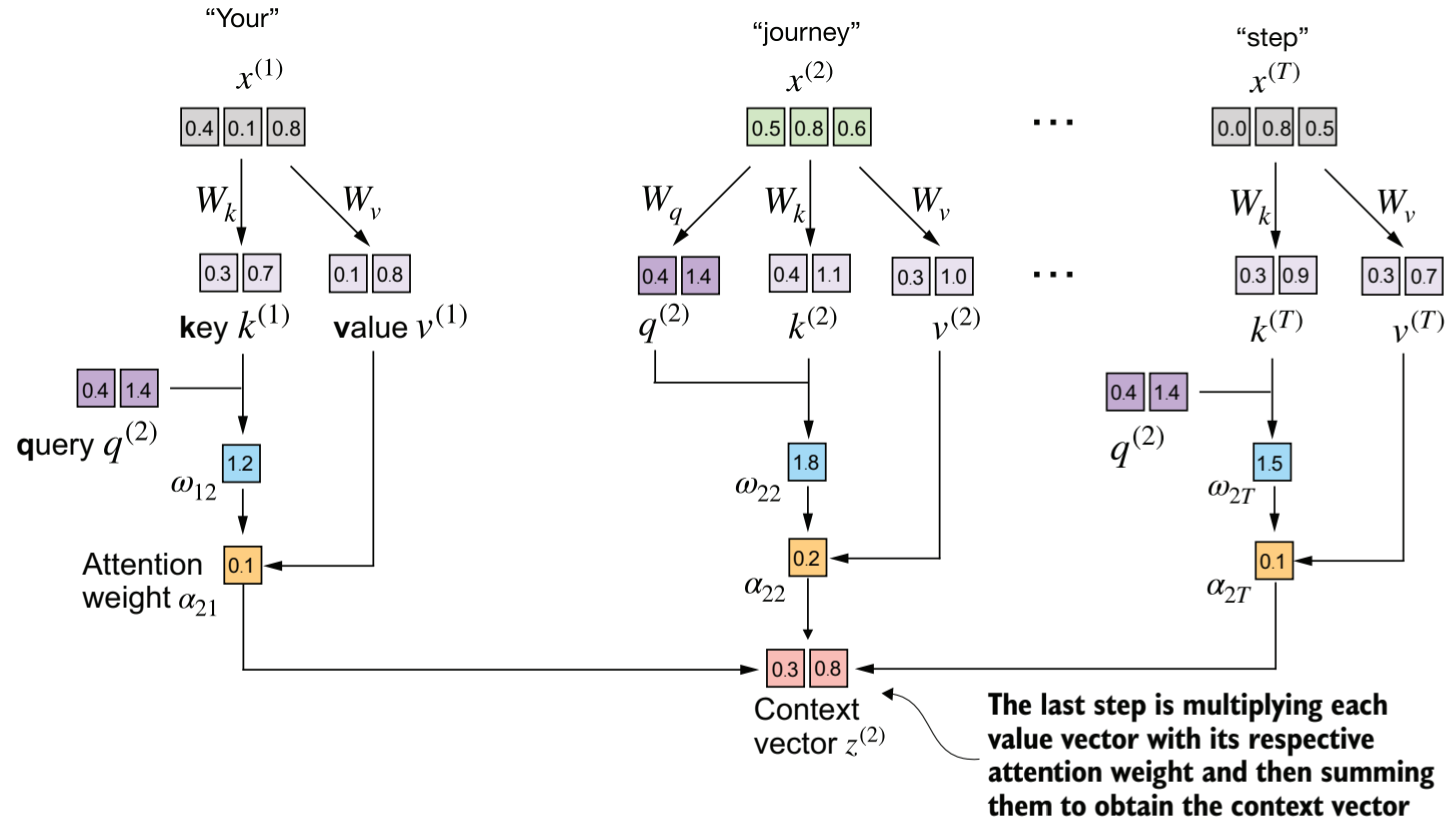
\includegraphics[width=1.0\linewidth]{./chapter2/media/TransformerAttentionKeyQueryValueSimply}
	\caption[Transformer: Self-attention computation]{Self-attention: Compute the new context vector of each input embedding vector by combining the (attention)-weighted value vectors. Image source:~\cite{Raschka2024BuildLLM}.}
	\label{fig:TransformerAttentionKeyQueryValueSimply}
\end{figure}

Instead of computing attention separately for each token, the Transformer performs the computation for the entire sequence using matrix operations~\cite{Raschka2024BuildLLM}, see \autoref{fig:TransformerSingleHeadAttention}. The matrix product $\mathbf{QK}^T$ computes the pairwise similarity scores between all tokens in the sequence in parallel, resulting in the attention score matrix.
\begin{equation}
	\mathbf{Z} = {Attention}(\mathbf{Q},\mathbf{K},\mathbf{V})=\text{softmax}\left( \frac{\mathbf{QK}^T}{\sqrt{d_k}} \right)\mathbf{V}
\end{equation}

\begin{figure}
	\centering
	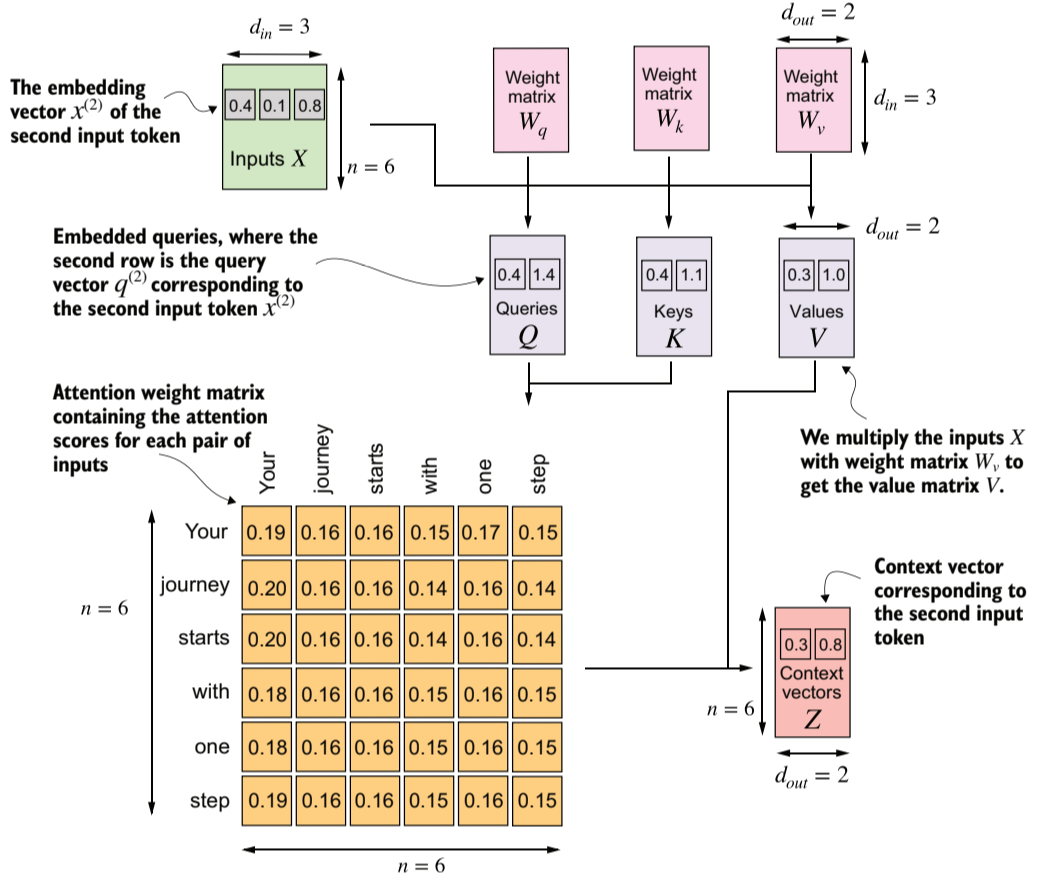
\includegraphics[width=0.8\linewidth]{./chapter2/media/TransformerSingleHeadAttention}
	\caption[Transformer: Self-attention computation]{Overview of a single self-attention block. Image source:~\cite{Raschka2024BuildLLM}.}
	\label{fig:TransformerSingleHeadAttention}
\end{figure}

% \paragraph{Multi-Head Self-Attention}
\textit{Multi-Head Self-Attention.} 
While a single attention mechanism can capture relationships between tokens, different types of dependencies may exist simultaneously within a sequence. To address this, the Transformer employs multi-head attention, which consists of several attention heads operating in parallel~\cite{Raschka2024BuildLLM, Vaswani2017AttentionIA}. Each head learns its own query, key and value projections and therefore focuses on different aspects of the input data. For example, one head may capture syntactic relationships, while another focuses on semantic dependencies. The outputs of all heads are concatenated and projected through a linear layer to form the final representation, see \autoref{fig:TransformerMultiHeadAttention}. This increases the model's ability to learn diverse linguistic patterns and contextual relationships.

\begin{figure}
	\centering
	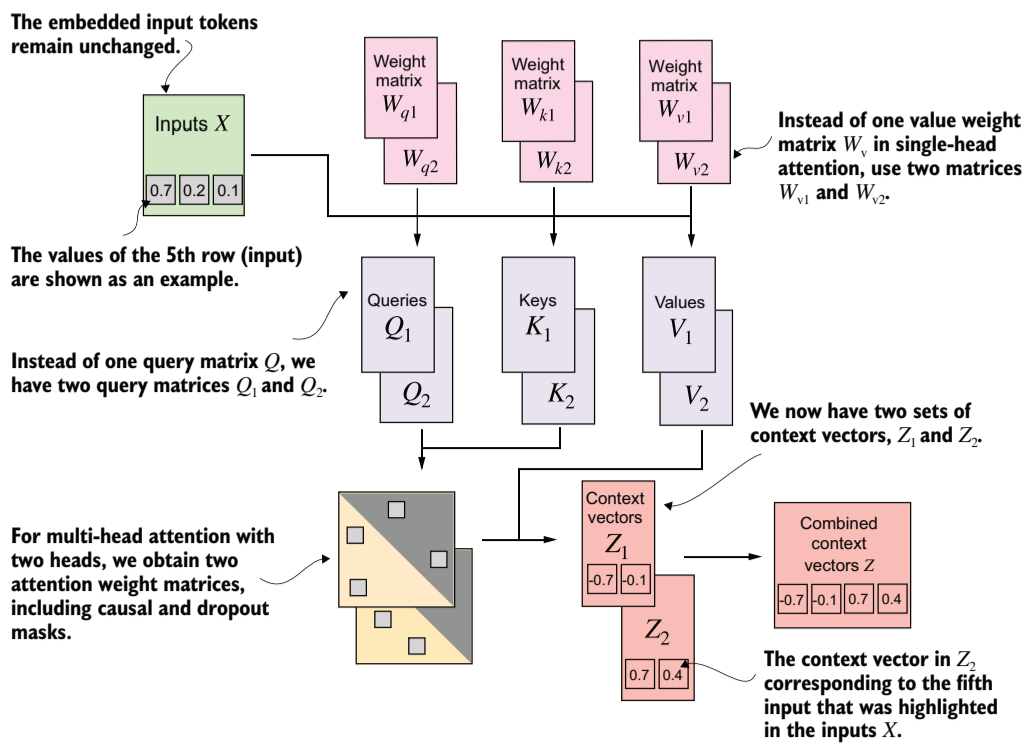
\includegraphics[width=0.8\linewidth]{./chapter2/media/TransformerMultiHeadAttention}
	\caption[Transformer: Multi-Head Attention Block]{Overview of a multi-head attention block. Image source:~\cite{Raschka2024BuildLLM}.}
	\label{fig:TransformerMultiHeadAttention}
\end{figure}


\paragraph{Encoder Block}
After the self-attention computation, the resulting representations are passed through a layer normalization step, followed by a \ac{MLP} Network. A second layer normalization is applied after this transformation. This sequence of operations forms a single Transformer block, which can be stacked multiple times to increase model capacity~\cite{Vaswani2017AttentionIA}.
The \ac{MLP} operates independently on each token representation. 
% In contrast to the attention mechanism, which is responsible for exchanging information between tokens, the \ac{MLP} refines and transforms each token embedding individually. 
It typically consists of two linear transformations with a non-linear activation function in between, allowing the model to learn more complex feature transformations.
A key component of the Transformer architecture is the use of residual connections, which are applied around both the attention block and the feed forward network and add the input of a sub-layer directly to its output~\cite{Vaswani2017AttentionIA}. This improves gradient flow during backpropagation and mitigates the vanishing gradient problem, which is especially important in deep networks composed of many stacked Transformer blocks. 

The output of the final encoder layer is a sequence of contextualized vectors, where each vector corresponds to one input token enriched with information from the entire sequence. This representation can then be used for downstream tasks such as classification, regression, or sequence generation.


\paragraph{Decoder Block}
The decoder receives an input sequence that is first transformed using the same embedding procedure as the encoder (token embeddings + positional information)~\cite{Vaswani2017AttentionIA}. During generation, this input typically consists of previously generated output tokens. The embedded sequence is then processed through two distinct attention mechanisms: masked multi-head self-attention and cross-attention.
% \paragraph{Masked Multi-Head Attention}
% \textit{Masked Multi-Head Attention.} 
Masked multi-head self-attention operates on the decoder's own input sequence, but with a causal mask that prevents each position from attending to any future positions~\cite{Raschka2024BuildLLM}. This ensures that every generated token depends only on its previous tokens.

In cross-attention, the decoder's hidden states from the masked attention layer serve as queries $Q$, while the encoder's output serve as keys $K$ and values $V$, allowing the decoder to condition its predictions on the encoded source sequence~\cite{Vaswani2017AttentionIA}.

After these attention layers, the resulting representations are passed through a linear projection head followed by a softmax function, producing a probability distribution over the set of possible output elements~\cite{Vaswani2017AttentionIA, Raschka2024BuildLLM, TransformerExplainerLLM}. The element with the highest probability (in our case the vocabulary token) is selected and appended to the generated sequence. This process repeats autoregressively until a special end-of-sequence symbol is produced. 
% In our text example, the vocabulary token with the highest probability is selected and appended to the generated sequence.







\section{Vision Transformer}
The Vision Transformer (ViT)~\cite{Dosovitskiy2020AnII} extends the Transformer architecture, originally developed for natural language processing, to computer vision tasks by applying the self-attention mechanism to image patches instead of words. In computer vision, attention enables a model to focus on relevant regions of an image and to capture and understanding relationships between different areas of an image. This allows the model to identify important objects and effectively model spatial dependencies across the entire image.

\begin{figure}[!h]
	\centering
	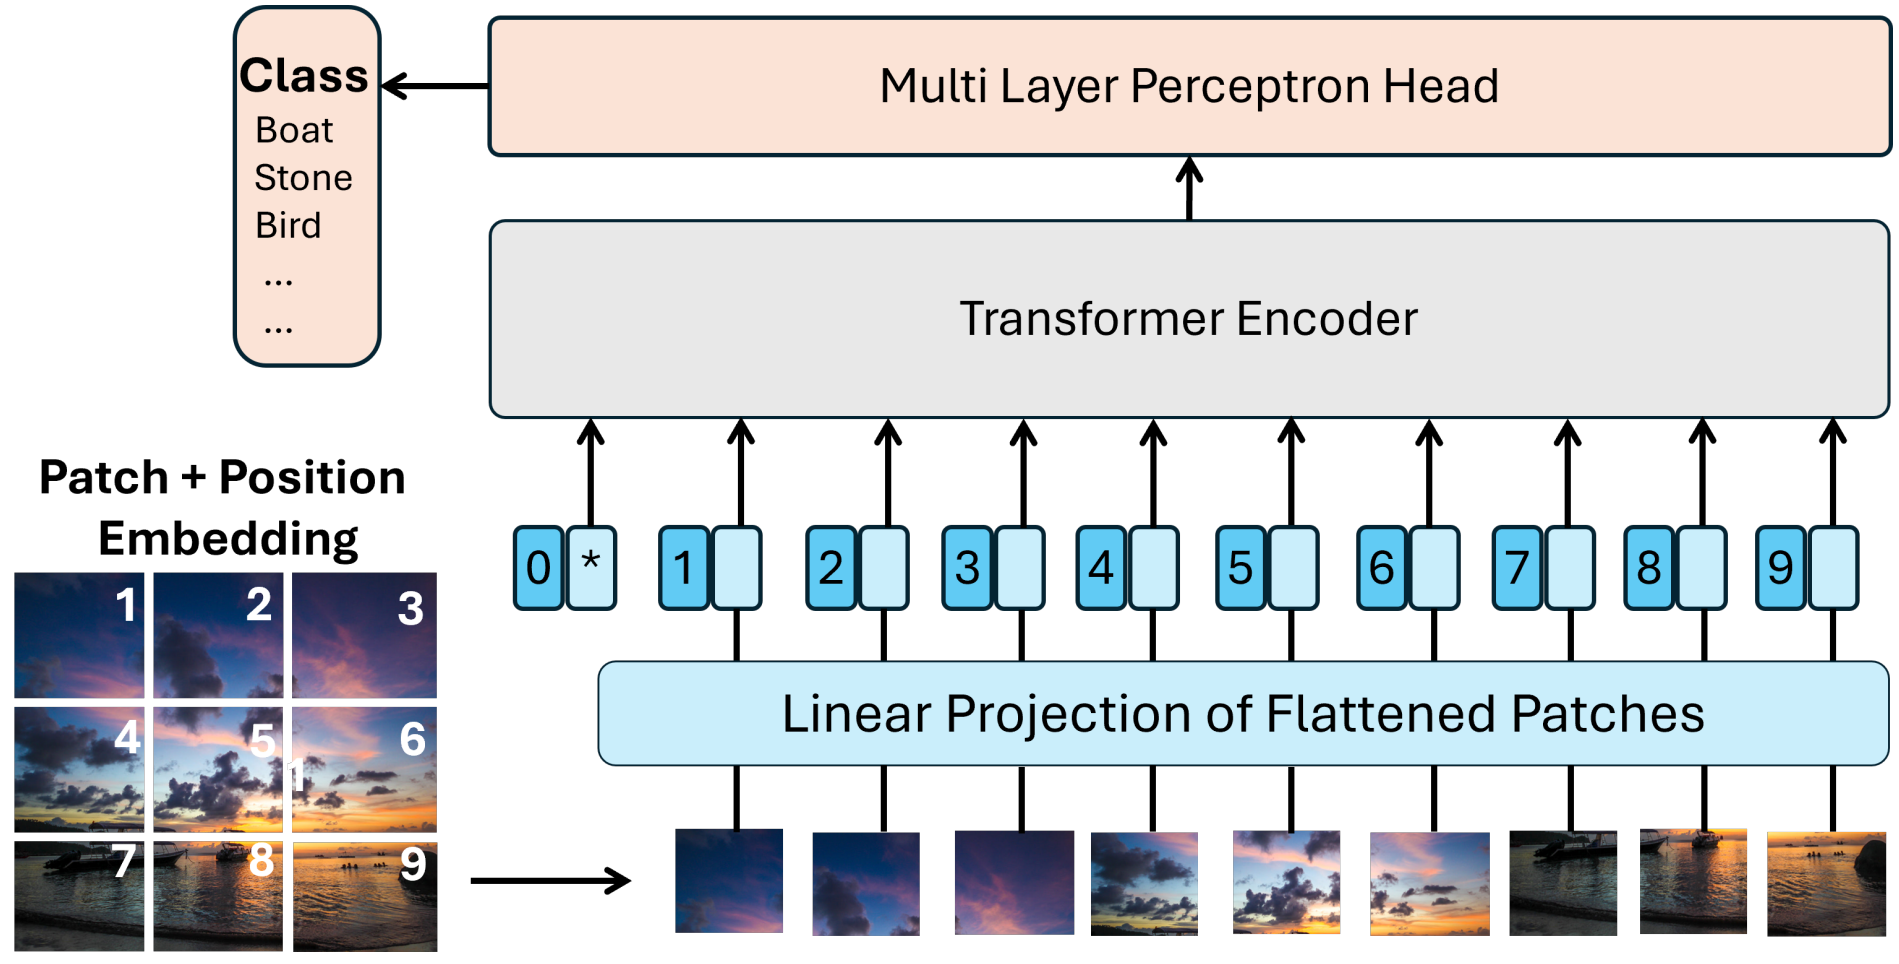
\includegraphics[width=0.6\linewidth]{./chapter2/media/VisionTransformerOverview}
	\caption[Vision Transformer Overview]{Vision Transformer: Overview of the architecture. Image source~\cite{Din2025VisionLA}.}
	\label{fig:VisionTransformerOverview}
\end{figure}

To process an image, ViT first divides the input image into a sequence of fixed-size, non-overlapping patches, see \autoref{fig:VisionTransformerOverview}. Each patch is flattened and linearly projected into a fixed-dimensional embedding vector, analogous to token embeddings in natural language processing.
Since the Transformer architecture does not inherently encode spatial information between the image patches, learnable positional embeddings are added to these patch embeddings. In addition, a learnable classification token (CLS token), denoted by an asterisk (*) in \autoref{fig:VisionTransformerOverview}, is prepended to the sequence and serves as a global representation of the whole image. During the attention computation, the CLS token interacts with all patch embeddings and gradually aggregates information from the entire image.
The resulting sequence is processed by a standard Transformer encoder consisting of multi-head self-attention and feed-forward layers. 
% Through self-attention, the model learns global relationships between image patches and can capture long-range spatial dependencies that are difficult to model with traditional CNN approaches. 
After the final encoder layer, the output representation of the CLS token serves as a global representation of the image and is passed through a multi-layer perceptron (MLP) head to generate the final prediction, such as class probabilities for image classification tasks.
% After the final encoder layer, the output representation of the CLS token contains information aggregated from all image patches and is passed to a multi-layer perceptron (MLP) head to produce the final prediction

Vision Transformers have demonstrated competitive performance on large-scale image classification benchmarks such as ImageNet~\cite{Deng2009ImageNetAL}, highlighting the effectiveness of attention-based architectures for visual representation learning~\cite{Dosovitskiy2020AnII}.
In imitation learning, Vision Transformers can be used as visual encoders that extract global scene representations from camera observations, which are subsequently used by the policy network to predict actions.







\section{Foundation Model}


% Recent advances in artificial intelligence have been largely driven by the development of foundation models. 
A foundation model is a large-scale model that is pre-trained on vast amounts of data and can subsequently be adapted to a wide range of downstream tasks~\cite{Bommasani2021OnTO}. Instead of being designed for a single application, foundation models learn general patterns, concepts and representations that can be reused across different domains and tasks.
A key characteristic of foundation models is their ability to generalize to problems that were not explicitly specified during training. This broad knowledge enables them to serve as a common basis for many specialized applications. 
Unimodal foundation models (e.g. GPT-3 for text~\cite{Brown2020LanguageMA}, Stable Diffusion for images~\cite{Rombach2021HighResolutionIS}) learn patterns within a single data type, whereas Multi-modal foundation models (e.g. CLIP~\cite{Radford2021LearningTV}, GPT-4V~\cite{Achiam2023GPT4TR}, Gemini~\cite{Reid2024Gemini1U, team2023gemini}) learn joint representations across modalities such as text, images and audio.
Due to their versatility and strong generalization capabilities, foundation models have become the foundation of many modern \ac{AI} systems.


% \begin{figure}[!ht]
% 	\centering
% 	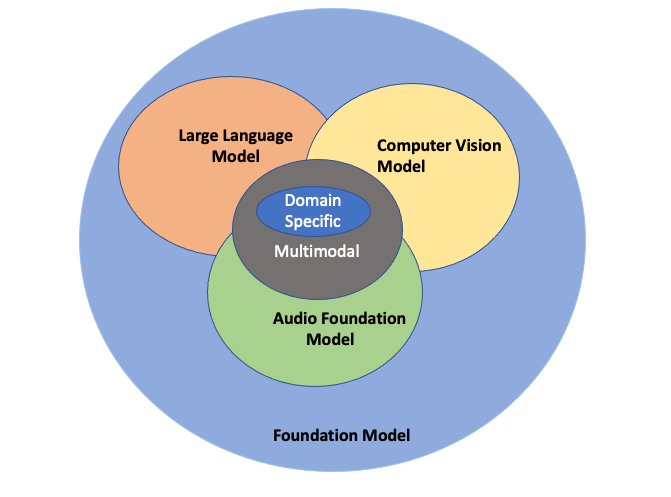
\includegraphics[width=0.55\linewidth]{./chapter2/media/FoundationModel_vs_MultiModalModel.png}
% 	\caption[Foundation Model vs. Multi-Model Model]{Foundation Model vs. Multi-Model Model. Image source:~\cite{FoundationModelsFoundation}}
% 	\label{fig:foundationmodel_vs_multimodel}
% \end{figure}

\section{Multi-Modal Model}
A multimodal model is capable of processing and relating information from two or more data modalities, such as text, images, audio, or sensor measurements~\cite{Baltruaitis2017MultimodalML}. Unlike unimodal models, which operate on only a single type of data, multimodal models learn a shared representation that enables information from different modalities to be interpreted jointly.
The integration of multiple modalities allows a model to leverage complementary information, handle missing data from one source by relying on another, provide more comprehensive insights and improves model generalization~\cite{Liang2022FoundationsT}.
For example, a multimodal model can analyze an image together with a textual instruction and use information from both inputs to answer a question or perform a task. 
Multimodal Learning is a own learning paradigm and refers to the use of various data modalities within a single learning concept~\cite{Ngiam2011MultimodalDL, Baltruaitis2017MultimodalML}.







\section{Reinforcement Learning} \label{sec:ReinforcementLearning}
\ac{RL} is both a fundamental discipline of \ac{ML} and a distinct approach within Robot Learning.
The robot learns a policy through trial and error using rewards provided from the given task and the environment. The actions performed by the agent are evaluated with a reward score and this score is then used to gradually optimize the policy. See also figure \ref{fig:RLConzept} for a general graphical overview. Below are the key terms in \ac{RL} explained in relation to robotics: 
\begin{itemize}
	\item \textbf{Agent:} The agent is the entity that learns to perform a specific behavior through interaction with its environment. In the context of this work, the agent corresponds to the robot, which has to execute a given action or task. 
	\item \textbf{Environment:} The environment is the setting in which the agent operates and is the workplace of the robot. In addition to the robot itself, it includes all relevant objects with which the robot interacts. The environment can be a simulated environment too.
	\item \textbf{Robot Actions $a$:} The Robot actions are simply the control commands the robot sends to its actuators, e.g. open or close the gripper, move to position $X,Y,Z$, joint angles, etc.
	\item \textbf{Reward $r$:} The reward is a numerical value that indicates how well the robot is performing in relation to the task objective. If the robot successfully picks up an object, it might receive a positive reward, while if it fails or drops the object, it might receive a negative reward. The goal of Reinforcement Learning is to learn a policy that maximizes the cumulative reward over time.
	\item \textbf{Robot State $s$:} The State is a complete description of the situation in the environment at a particular point in time. 
	% The robot state represents the current situation of the robot and its environment. 
	It can include various types of information, such as the robot's position, orientation, joint angles, sensor readings and even visual input from cameras~\cite{walkerastroActionSpaceState2024}. The state is crucial for the robot to make informed decisions about which actions to take.
	\item \textbf{Observation $o$:} An observation is the information that the robot receives from its sensors at a given time step. It may not provide a complete picture of the environment and thus may not fully represent the true robot state. In our case, the observation is mostly equivalent to the state~\cite{walkerastroActionSpaceState2024}. The observation can for example include the last camera frames as well as additional sensor inputs such as proprioceptive signals from the robot.
	\item \textbf{Policy $\pi$:}
	The policy can be interpreted as the brain of the agent and controls the robot's motion. The policy determines which action should be taken next when the agent is in a particular state in order to achieve the task objective. 
	% The Policy controls the robot's motion and actions. 
	Formally, a policy can be represented as  
	\begin{align}
		\pi_\theta(a \mid s)  
	\end{align}
	which defines a probability distribution over actions $a$, conditioned on the current state $s$. In other words, the policy specifies how likely the agent is to select a particular action given its current observation of the environment. 

\end{itemize}





\paragraph{Markov Decision Process}

\ac{RL} is based on the \ac{MDP}. A \ac{MDP} is a stochastic decision-making process that formally models the transition probabilities from a state $s$ to a subsequent state $s'$ provided that action $a$ is performed, expressed mathematically as $P(s'|s,a)$~\cite{sutton2018reinforcement, millerMarkovDecisionProcesses}. 
The objective is to learn a policy $\pi(a|s)$ that maximizes the expected long-term cumulative reward, defined as $\mathbb{E}\left[\sum_{t=0}^{\infty} \gamma^t r_t\right]$. The discount factor $\gamma \in [0,1]$ determines the importance of future rewards compared to immediate rewards. A value of $\gamma$ close to 0 makes the agent focus more on immediate rewards, while a value close to 1 encourages the agent to consider long-term rewards more heavily~\cite{sutton2018reinforcement, jagtapUnderstandingMarkovDecision}.
A \ac{MDP} also defines the reward function $R_a(s,s')$ that specifies the reward $r$ an agent receives when taking action $a$ in state $s$ and transitioning to a subsequent state $s'$~\cite{sutton2018reinforcement, millerMarkovDecisionProcesses}.
%  This is commonly expressed as $R_a(s,s')$~\cite{sutton2018reinforcement, millerMarkovDecisionProcesses}.

The \textbf{Markov property} says that all information from the past is contained in the current state, mathematically expressed as $P(s_{t+1}|s_{t}) = P(s_{t+1}|s_{1},s_{2}, ... s_{t})$. In other words, the transition probabilities depend only on the current state and not on the history of previous states~\cite{jagtapUnderstandingMarkovDecision}.
In practice, the Markov property is often not strictly satisfied. For example, a single image captured by a camera does not provide sufficient information to infer the dynamics of the environment. From one image alone, it is not possible to determine whether a car is moving forward at 100 km/h or 10 km/h, reversing, or remaining stationary. However, such information is crucial for making correct decisions in applications like autonomous driving~\cite{staffWhatMarkovDecision2025}.
Therefore, in practice, only sufficiently informative state representations are often used because the ideal Markov property is not strictly fulfilled. In the example above, the sequence of the last camera frames can be used.
%  to better capture the underlying dynamics of the environment~\cite{millerMarkovDecisionProcesses}.



\paragraph{Training Process}
At the beginning of the training process, a randomly initialized policy leads the robot to perform random movements. Through this interaction with the environment, the agent explores different actions and attempts to identify those that yield high rewards. Actions associated with higher rewards are subsequently assigned a higher probability by the policy, making the robot more likely to select them in similar situations in the future.

A successful learning process requires a suitable balance between exploration and exploitation. 
Exploration involves trying new or infrequently selected actions to gather information about the environment, while exploitation focuses on selecting actions that have previously yielded high rewards. Early in training, exploration is emphasized to discover effective behaviors, whereas later stages increasingly rely on exploitation to maximize task performance.

Numerous methods and algorithms have been proposed to effectively balance exploration and exploitation, $\epsilon$-greedy strategy, Upper Confidence Bound (UCB) and Thompson Sampling. 
% However, a detailed discussion of these methods is beyond the scope of this thesis.
Due to the exploration phase, the success of the chosen \ac{RL} approach only becomes visible at a late stage, unlike in classical deep learning, see Figure \ref{fig:trainingprogressdlandrl}. 


\begin{figure}[!ht]
	\centering
	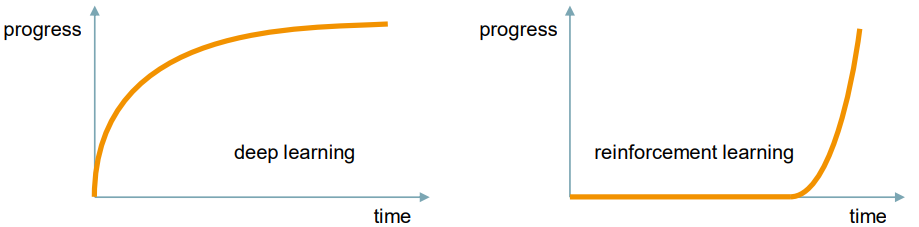
\includegraphics[width=0.7\linewidth]{./chapter3/media/TrainingProgressDLandRL.png}
	\caption[Training Progress in Deep Learning and Reinforcement Learning]{The task success in \ac{RL} becomes visible at a later stage compared to deep learning due to the exploration phase. Image source:~\cite{KontaktNierhoff}}
	\label{fig:trainingprogressdlandrl}
\end{figure}











% \subsection{Knowledge Modalities from Video}
\paragraph{Knowledge Modalities from Video}
An \ac{RL} \ac{KM} is some function learned from data that represents specific types of \ac{RL}-related knowledge.
\ac{KM}s can be learned through trial-and-error principles or from video datasets~\cite{Wulfmeier2023FoundationsFT}:
%  can capture different aspects of the \ac{RL} problem~\cite{Wulfmeier2023FoundationsFT}. 

\begin{itemize}
	\item \textbf{Policy:} The policy specifies how likely the agent is to select a particular action given its current observation of the environment.
	It can be learned from video data by observing the actions taken in different states and learning to predict those actions based on the visual input~\cite{Wulfmeier2023FoundationsFT}. 
	
	\item \textbf{Value functions:} Value functions estimate the expected future return (cumulative reward) for a given state~\cite{sutton2018reinforcement}, see Figure \ref{fig:VFunctionVsQFunction}. They can be learned from video data by observing the outcomes of actions and learning to predict the expected future rewards based on the visual input~\cite{Wulfmeier2023FoundationsFT}.

	\begin{itemize}
		% V-Function
		\item \textit{State-value function (V-function):} 
		A V-function $V_\pi(s_t)$ is a mapping from states to the expected future return when acting under a particular policy $\pi$~\cite{sutton2018reinforcement}. $V_\pi(s)$ does not provide information about the quality of individual actions available in that state $s$. 
		Intuition: ''How good is it to be a certain state, if I follow my policy $\pi$?''

		% \begin{figure}[!ht]
		% 	\centering
		% 	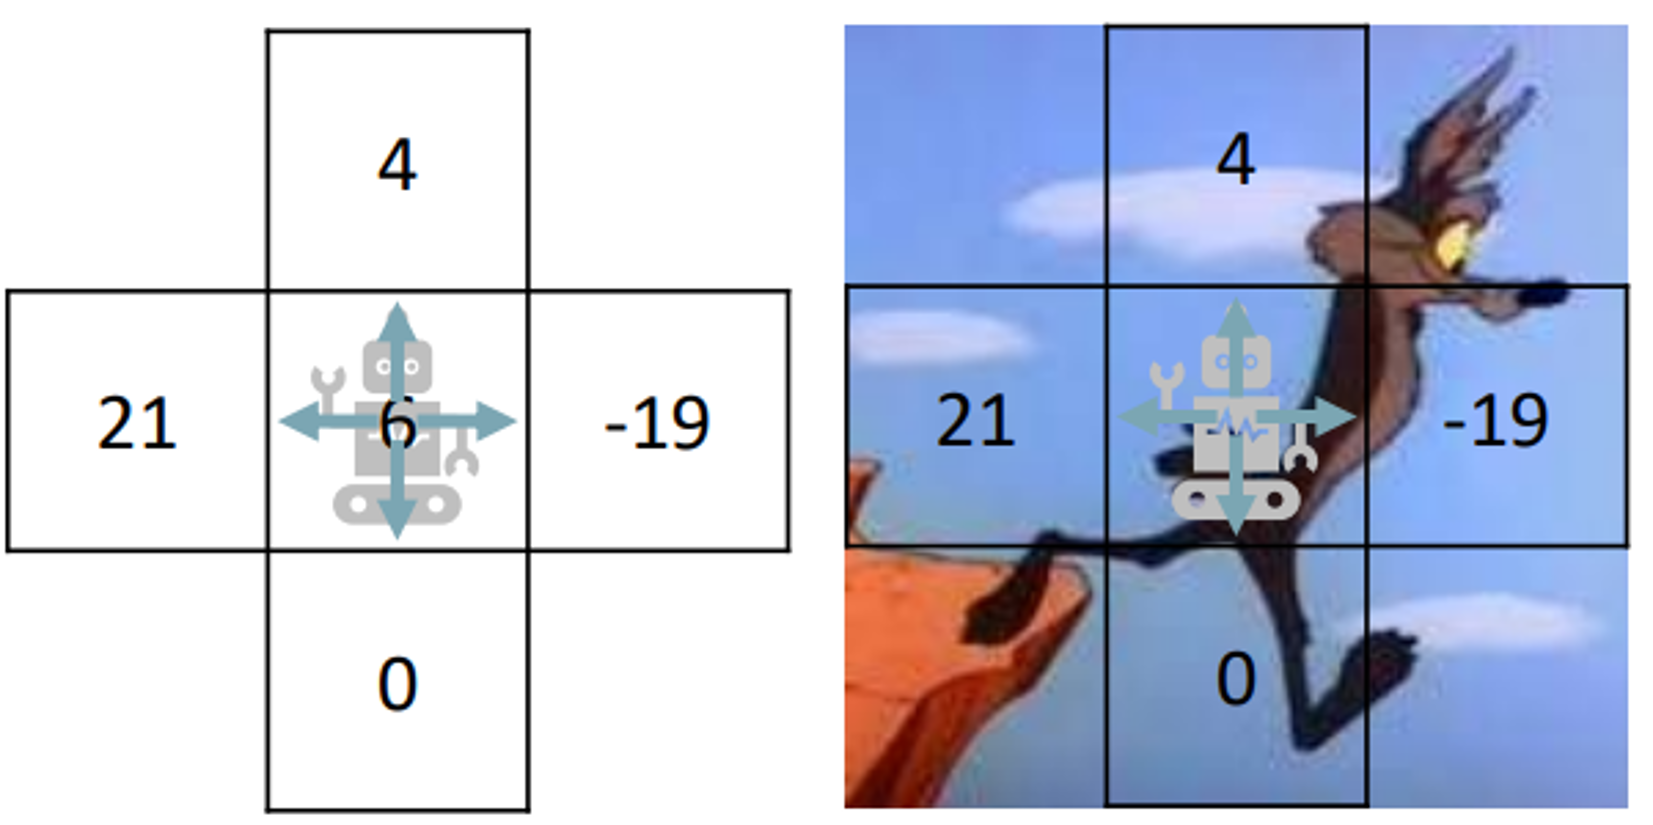
\includegraphics[width=0.55\linewidth]{./chapter3/media/V_Function.png}
		% 	\caption[State-Value Function]{State-Value Function}
		% 	\label{fig:statevaluefunction}
		% \end{figure}

		% Q-Function
		\item \textit{State-action value function (Q-function):} 		
		A Q-function $Q_\pi(s_t,a_t)$ is a mapping from state-action pairs to the expected future return when acting under a particular policy $\pi$~\cite{sutton2018reinforcement}. $Q_\pi(s,a)$ evaluates the expected return of taking a specific action $a$ in state $s$ and subsequently following the policy $\pi$. It provides information about the quality of individual actions available in that state $s$.
		Intuition: ''How good is this specific action in a certain state, if I continue behaving like my policy $\pi$?''

		% \begin{figure}[!ht]
		% 	\centering
		% 	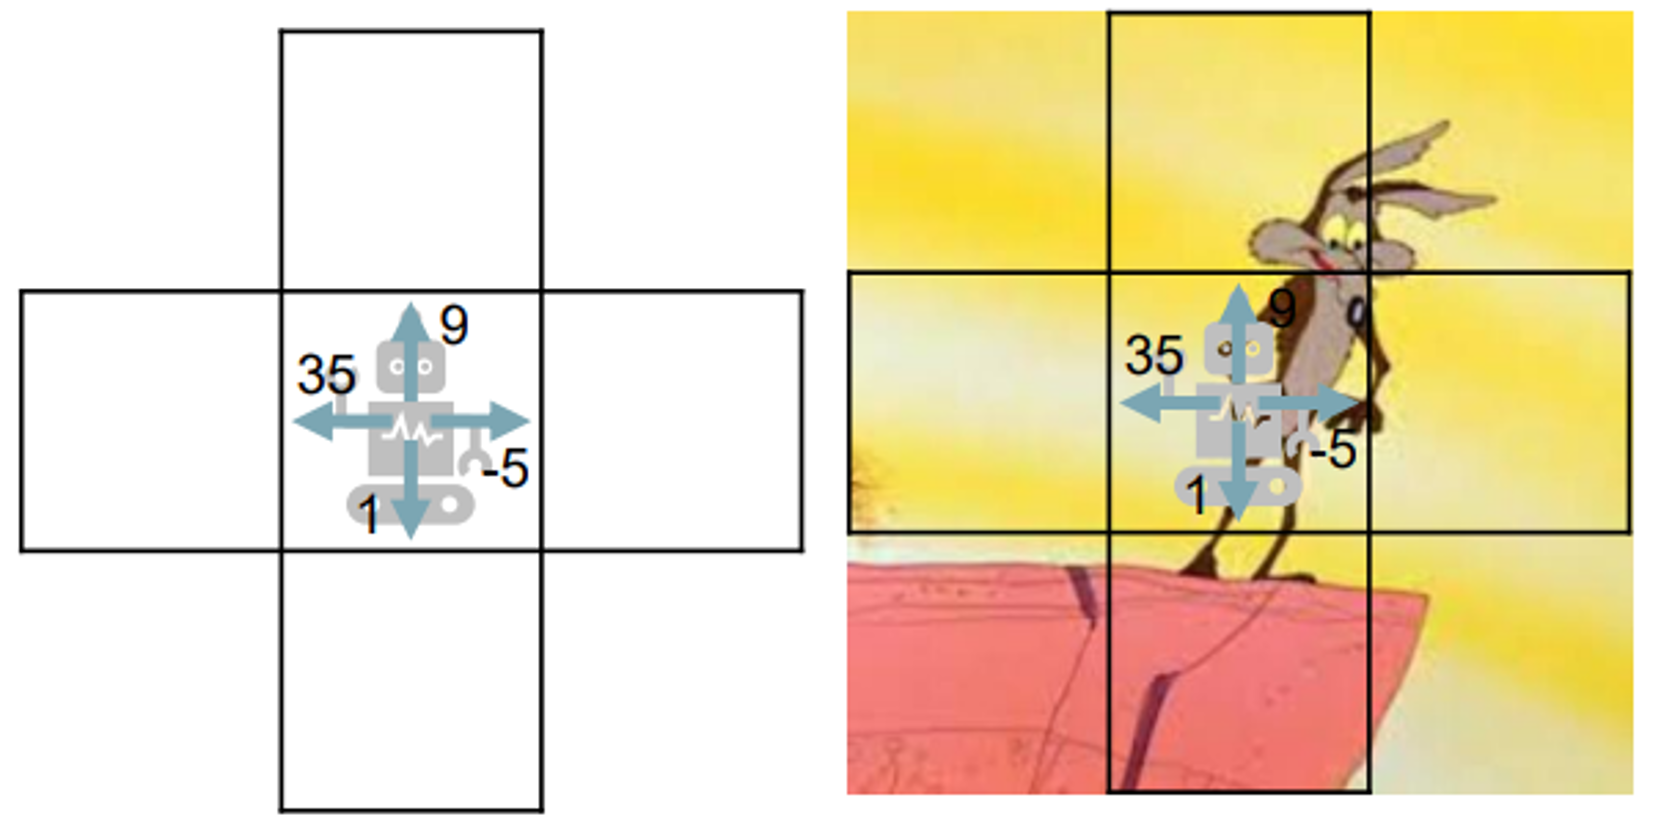
\includegraphics[width=0.55\linewidth]{./chapter3/media/Q_Function.png}
		% 	\caption[State-Action Value Function]{State-Action Value Function}
		% 	\label{fig:stateactionvaluefunction}
		% \end{figure}

		

	\end{itemize}
	
	\begin{figure}[h]
		\centering
		\subfigure[V-Function: Returns the expected future return for a given state.]{
				\begin{minipage}{6.3cm} % subfigure box width
				\centering
				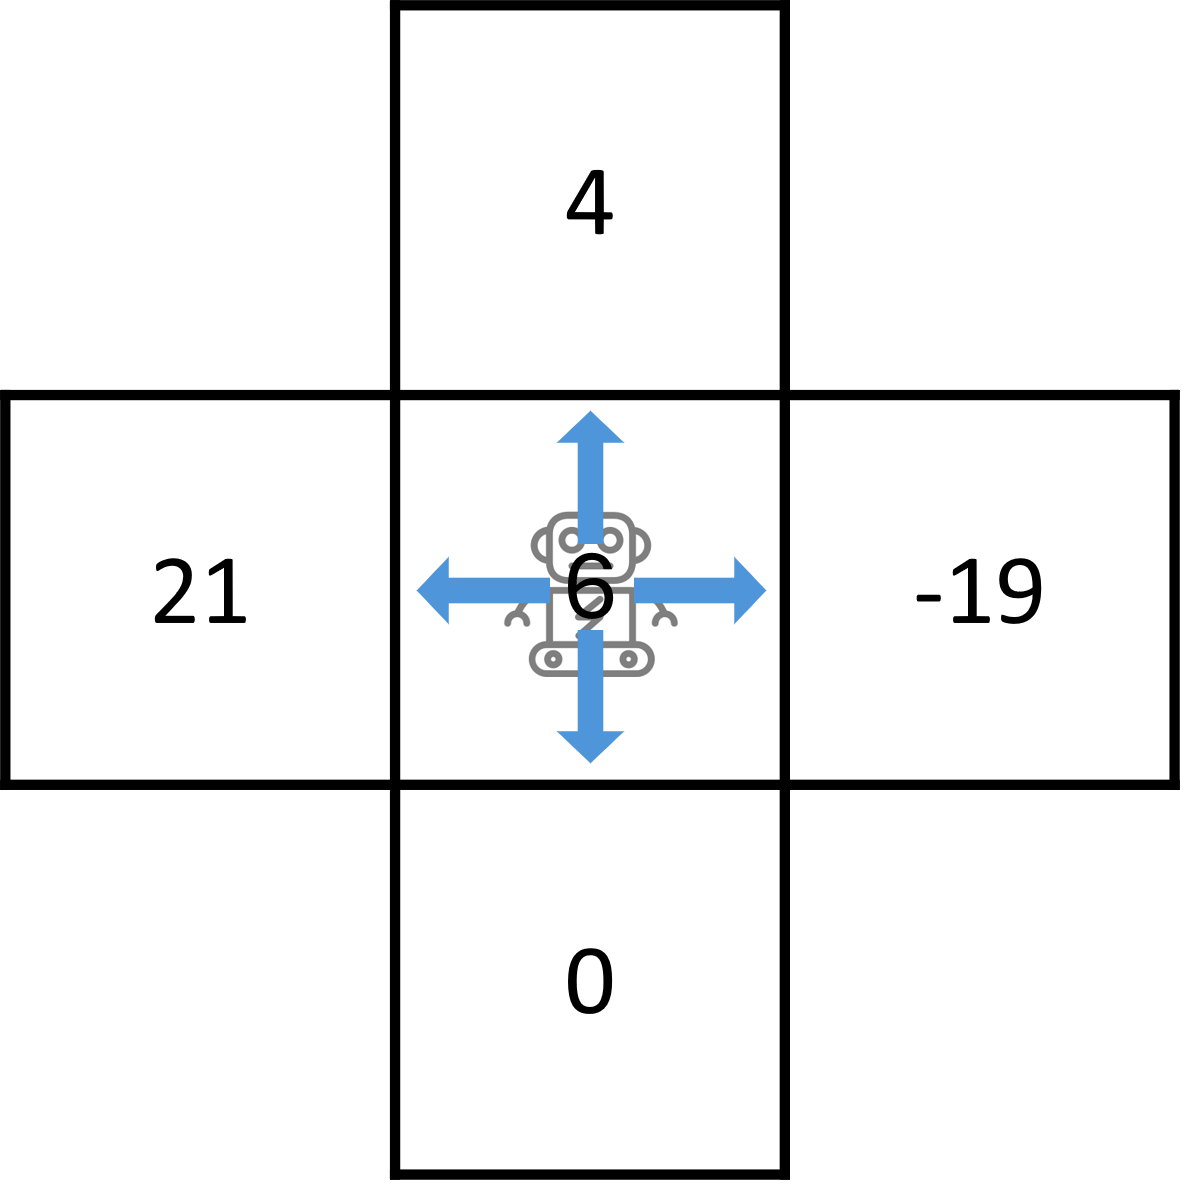
\includegraphics[width=4.6cm]{./chapter2/media/RL_VFunction.png}
				\label{fig:RL_VFunction}
			\end{minipage}%
		}
		\hspace{0.8cm}
		\subfigure[Q-Function: Returns the expected future return for a given state-action pair.]{
			\begin{minipage}{6.3cm} % subfigure box width
				\centering
				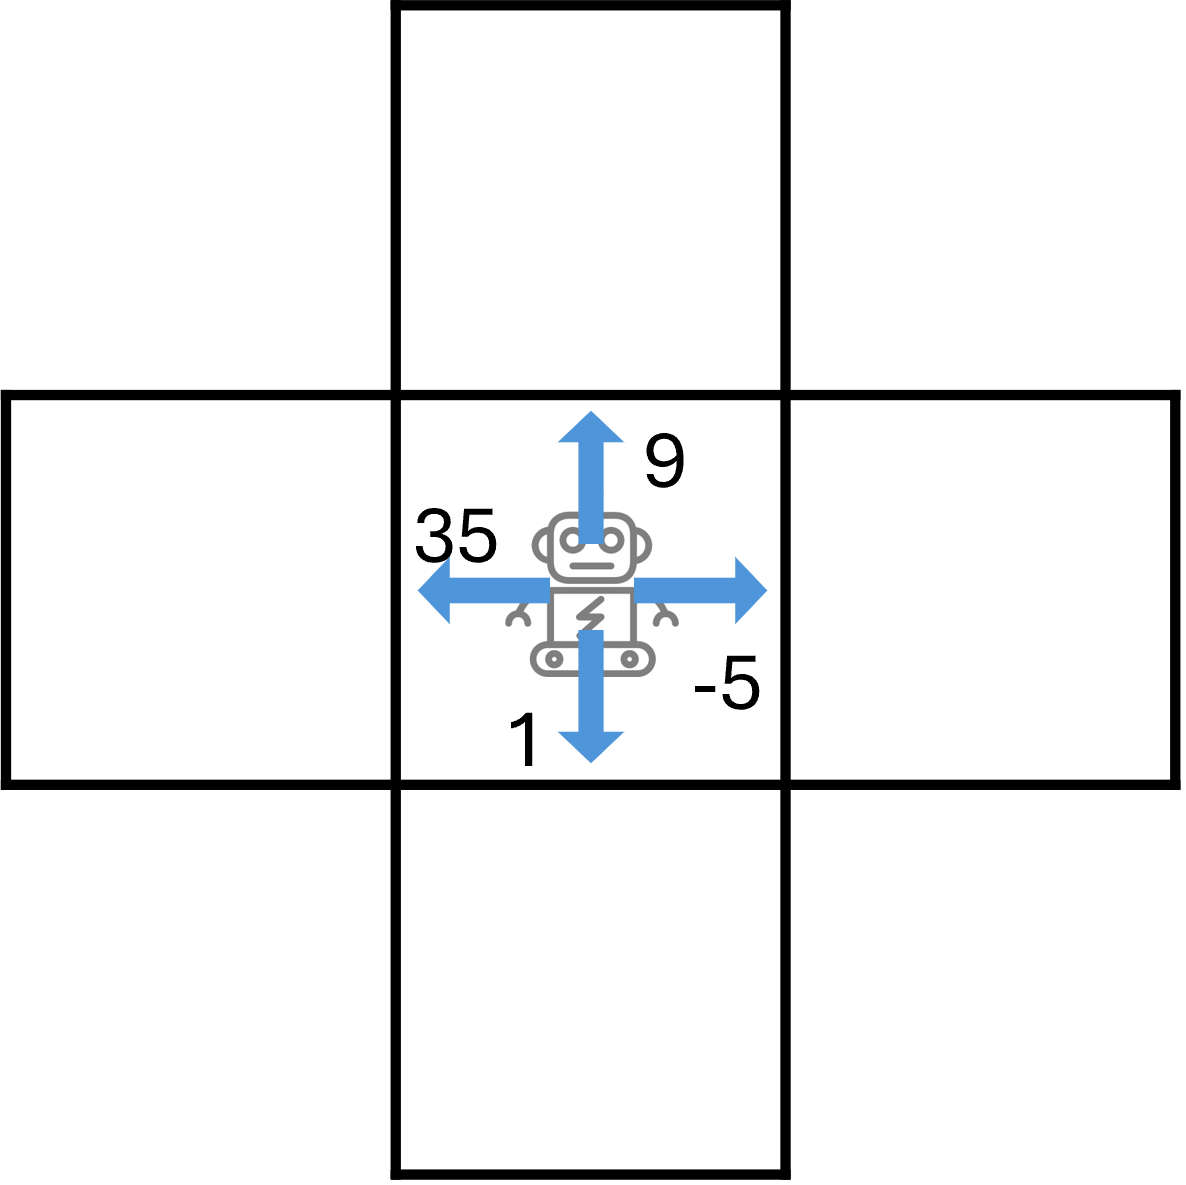
\includegraphics[width=4.6cm]{./chapter2/media/RL_QFunction.png}
				\label{fig:RL_QFunction}
			\end{minipage}%
		}
		\caption[Comparison of V-Function and Q-Function.]{Comparison of V-Function and Q-Function. The V-Function estimates the expected return for a given state, while the Q-Function estimates the expected return for a given state-action pair. Image based on~\cite{KontaktNierhoff}}
		\label{fig:VFunctionVsQFunction}
	\end{figure}


	% Dynamics model:
	\item \textbf{Dynamics model:} A Dynamics model $p(s_{t+1}|s_t,a_t)$ predicts the next state $s_{t+1}$ given the current state $s_t$ and action $a_t$~\cite{sutton2018reinforcement}. 
	% Video prediction models can be used as robot dynamics models~\cite{Eze2024LearningBW}. 
	By learning to predict future video frames based on current observations and actions, the model can capture the underlying dynamics of the environment and allows the robot to anticipate the consequences of its actions and make informed decisions based on predicted future states~\cite{Eze2024LearningBW}.
	% Reward model:
	\item \textbf{Reward model:} A reward function $r(s_t,a_t)$ defines the reward received by the agent for taking action $a_t$ in state $s_t$~\cite{sutton2018reinforcement}. It can be learned from video data by observing the outcomes of actions and inferring the underlying reward structure that motivates those actions. For example, if a video shows a robot successfully picking up an object, the reward function can learn to assign a positive reward to that action in similar states.
\end{itemize}





\section{Imitation Learning} \label{sec:ImitationLearning}
\ac{IL} or Learning from Demonstration is a general term for methods in which the agent derives or learns its behavior from expert demonstrations or ``in the wild'' videos~\cite{Chrysomallis2025ImitationLI}. ``In the wild'' videos refer to videos that are not specifically recorded for training purposes, but are instead sourced from real-world settings, such as those found in great variety on the internet, for example on platforms like YouTube.
% \ac{IL} makes it possible to use "in the wild" videos—such as those found in great variety on the internet, for example on platforms like YouTube — to train \ac{AI} models~\cite{McCarthy_2025}.
The demonstration videos can show a robot, a human, or even a loose sequence of actions, both in the real world or in a simulation environment, performing a specific task. However, videos without a clearly defined objective or with unknown activity can also be used~\cite{McCarthy_2025}.
Models can through \ac{IL} be trained to capture the visual and semantic relationships, as well as the physical dynamics of the real world. This in turn is a key prerequisite for the development of a generalist policy. 
\ac{IL} can be divided into Behavior Cloning (\autoref{sec:BehaviorCloning}) and Learning from Videos (\autoref{sec:LearningfromVideos}).


\paragraph{Idea Behind Imitation Learning} 
When people want to learn a new skill, they often turn to how-to videos. They learn the new skill through speech instructions and visual observations in the video~\cite{Jain2024Vid2RobotEV}. The same principle is now to be applied to robots through \ac{IL}.
Visual Imitation Learning is particularly well suited for teaching tasks that are difficult or impossible to specify through language alone.
It allows robots to infer task-relevant actions from demonstrations performed in different environments and can be more data-efficient than \ac{RL}, especially in high-dimensional state spaces and complex environments. Furthermore it benefits from large-scale human demonstration datasets, which are often easier to collect than robot-specific expert demonstrations in the specific domain\cite{Jain2024Vid2RobotEV}.
% Visual Imitation Learning ...
% \begin{itemize}
%     \item is ideal for teaching tasks that are difficult or impossible to describe in words.
%     \item allows robots to infer tasks from expert demonstrations in different environments than the robot.
%     \item can be more data efficient than \ac{RL}, especially in high-dimensional state spaces, like a complex robot environment. 
%     \item can leverage large datasets of human demonstrations, which are often easier to collect than expert demonstrations in the specific domain~\cite{Jain2024Vid2RobotEV}.
% \end{itemize}

% \texttt{Problems in RL:}
In \ac{RL} a task is commonly defined through a reward function, which assigns a high reward to desirable behavior and a low reward to undesirable behavior~\cite{sutton2018reinforcement}. However, designing good reward functions is challenging for every task and many methods based on computer vision rely on annotated demonstrations in every new environment~\cite{McCarthy_2025}. \ac{IL} allows us to learn complex behaviors that are difficult to specify through a reward function, or it can help us to define a good adaptive reward function for \ac{RL}.


\subsection{Behavior Cloning}
\label{sec:BehaviorCloning}
\ac{BC} is a fundamental approach within \ac{IL}, where a policy is learned directly from annotated expert demonstrations~\cite{Eze2024LearningBW}. The training data consists of state-action pairs $(s_t, a_t)$ and the problem is formulated as a standard supervised learning task.  
Conceptually, \ac{BC} can be understood as a form of direct imitation or copying of expert behavior, without explicitly modeling the underlying system dynamics or task objectives. 
% Due to its simplicity and scalability, BC is one of the most widely used methods in robot learning from datasets.  
% BC is used to train Vision Language Action models and for pre-training models used in \ac{RL}, see Section \textbf{XXX}

% \paragraph{Purpose: Policy Learning} 
Formally, \ac{BC} learns a policy $\pi_\theta(a_t \mid s_t)$ by supervised learning on expert demonstrations.
% :
% \begin{align}
% 	\pi_\theta(a_t \mid s_t)
% \end{align}
% where:
% \begin{itemize}
% 	\item $s_t$: State / Observation (images, proprioception, etc.) at time $t$
% 	\item $a_t$: Expert action at time $t$
% \end{itemize}
The Policy is optimized by minimizing the prediction error between the actions generated by the model and the corresponding expert actions;
\begin{equation}
	\min_{\theta} \mathbb{E}_{(s_t,a_t) \sim \mathcal{D}} \left[ \mathcal{L}(\pi_{\theta}(s_t), a_t) \right]
\end{equation}
where $\mathbb{E}_{(s,a) \sim \mathcal{D}} [\cdot]$ means taking all state-action pairs $(s, a)$ inside the expert dataset $\mathcal{D}$ and calculating the average prediction loss.
% where:
% \begin{itemize}
% \item $\pi_{\theta}(s)$: The action your robot's policy predicts given state $s$.
% \item $a$: The actual action the expert took in that same state.
% \item $\mathcal{L}$: Usually Mean Squared Error (MSE) for continuous control or Cross-Entropy for discrete actions.
% \item  $\mathbb{E}_{(s,a) \sim \mathcal{D}} [\cdot]$: Take all the state-action pairs $(s, a)$ inside the expert dataset $\mathcal{D}$ and calculate the average value of the expression inside the brackets.
% \end{itemize}
 







  
\subsection{Learning from Videos}
\label{sec:LearningfromVideos}
\ac{LfV}, also referred to as \ac{LfO}, relies solely on video demonstrations without explicit action annotations~\cite{McCarthy_2025, Burnwal2025LearningFO}. In contrast to \ac{BC}, where state-action pairs are directly available, \ac{LfV} aims to infer the underlying actions or high-level intent purely from perceptual data, i.e. mapping observations to actions $(s \rightarrow a)$. It often uses Representation Learning, to learn and discover the most important (unknown) underlying data characteristics.% by transforming and reducing input in a fully data-driven and automatic manner.	

A central challenge in \ac{LfV} is determining which actions correspond to the observed behavior in the video~\cite{McCarthy_2025}. Since no action labels are provided, additional methods and techniques are required to recover or approximate the missing action information. See \autoref{chap:LearningFromVideosDataModalityAndChallenges} for more information.
Due to this property, \ac{LfV} can be seen as a weakly supervised or self-supervised \ac{IL} approach. 
Its main advantage lies in scalability, as it enables leveraging large amounts of unannotated video data without the need for costly data annotation~\cite{McCarthy_2025}. Furthermore, additional actions can be derived from annotated video data too~\cite{McCarthy_2025}.
In robotics, \ac{LfV} is commonly used as a pretraining step. The learned representations capture visual, semantic and dynamical aspects of the environment, which can later be refined using methods such as \ac{BC} with annotated data or in \ac{RL}~\cite{McCarthy_2025}. This combination allows models to first learn the real worlds dynamics from large-scale video data and subsequently specialize on task-specific robot demonstrations.

%BC is used to pre-train models for Behavior Cloning and Reinforcement Learning, see Section \textbf{XXX} for more information.

% \paragraph{Purpose: Inferring Actions}
Formally, \ac{LfV} learns to infer actions from observations in a weakly supervised or self-supervised manner:
\begin{align}
	a_t = f(s_t, s_{t+1})
\end{align}
where $a_t$ is the ``latent'' or predicted action and $f$ the inverse dynamics function (often a neural network) that maps state transitions to actions.
% \ac{LfV} learns to infer actions from observations in a weakly supervised or self-supervised manner. 
% \begin{align}
% 	a_t = f(s_t, s_{t+1})
% \end{align}
% where:
% \begin{itemize}
% 	\item $a_t$: The "latent" or predicted action.
% 	\item $s_t$: The current state/video frame.
% 	\item $s_{t+1}$: The next state/video frame.
% 	\item $f$: The inverse dynamics function (often a neural network) that maps state transitions to actions.
% \end{itemize}


  \chapter{Generalist Robots and the Data Bottleneck}
\minitoc
This Chapter descripes the overall goal of Robotics, to develop an generalist robot that can perform a wide variety of tasks in unstructured, unseen real-world environments. It also introduces to the data bottleneck in robotics, which arises from the limited availability of large, diverse, and high-quality datasets and hinders the development of an generalist robot. The chapter discusses different data sources for robot learning, including real-world robot data, simulated data, and internet data, and highlights the challenges and opportunities associated with each source. Finally, it emphasizes the importance of leveraging large-scale internet video data to address the data bottleneck and improve robotic learning capabilities.
% Classical robotics techniques are insufficient as they cannot handle unseen and unstructured scenarios \cite{Krotkov_DARPA_2017}.


\section{Generalist Robots}
The ultimate goal of robotics is to develop a \textbf{generalist robot}. According to McCarthy et al. \cite{McCarthy_2025}, such a robot should be able to perform a wide variety of physical tasks in unstructured, unseen real-world environments. It must combine high-level reasoning and planning abilities with low-level physical skills, such as dexterous manipulation. Furthermore, it should be capable of adapting to unforeseen situations and operate under imperfect and partial observations, for example through visual and tactile sensing. In summary, a general-purpose robot is capable of adapting to different situations and learning new skills just like humans \cite{tsujiSurveyImitationLearning2026}. Such a robot would be highly useful across a wide range of real-world applications. 

\paragraph{Application Field: Industrial Settings}
In industrial settings, this would enable robots to be deployed flexibly across different environments and tasks, without the need for task-specific or environment-specific programming or retraining. As a result, robots could also be utilized for spontaneous small, short-term tasks, where automation is currently not economically viable due to high setup costs and effort. This increased flexibility would lead to higher utilization rates and, consequently, reduced long-term operational costs \cite{tsujiSurveyImitationLearning2026}.

\paragraph{Application Field: Household Settings}
In addition, general-purpose robots could play an important role in household settings. They could assist with everyday tasks such as tidy up rooms, loading/unloading dishwashers, setting tables, or acting as general assistants for example helping to carry objects.

\paragraph{Application Field: Healthcare and Assistive Settings}
In healthcare and assistive contexts, such robots could support individuals with limited mobility by helping them perform daily activities, such as standing up, sitting down, opening a door, or transporting objects. This highlights the potential of generalizing robotic systems to improve both efficiency in industry and quality of life in everyday and care settings \cite{tsujiSurveyImitationLearning2026}.

\subsection{Ethical Concerns} 
Ethical concerns regarding the development of generalist robots should not be underestimated and must not be ignored. In the future, robots are likely to take over many tasks, particularly those that are repetitive and monotonous, which may lead to the displacement of certain jobs. Whether this could result in large-scale unemployment due to automation remains a subject of ongoing debate.

Furthermore, once the technology has sufficiently matured, such robots could also be used for \texttt{military purposes}. While this could reduce the risks to human soldiers, it also raises serious ethical concerns, as it makes forms of automated or autonomous warfare increasingly conceivable.

It is therefore essential that the development and deployment of generalist robots are carried out responsibly and in accordance with ethical guidelines, in order to minimize potential negative impacts on society.


\section{Data Bottleneck in Robotics}
A central question in robotics is how to train a generalist robot capable of performing a wide range of tasks in unstructured and previously unseen real-world environments?

\textit{Usage of Large-Scale Datasets.} Progress in related machine learning domains—such as Natural Language Processing \cite{Achiam2023GPT4TR}, Computer Vision \cite{betkerImprovingImageGeneration}, and video generation \cite{videoworldsimulators2024}—suggests that large-scale datasets and model capacity are key drivers of performance and generalization capabilities. 
Training high-capacity models with expressive architectures on diverse, extensive internet-scale datasets has led to the emergence of robust representations and improved out-of-distribution performance in these domains \cite{Vaswani2017AttentionIA}.
Empirically, these improvements often follow predictable scaling laws, where performance improves as more data, model size, and compute are used \cite{kaplan2020scalinglawsneurallanguage}.
Recent work suggests that similar scaling behavior may also apply to robotics and \ac{IL}. For example, studies show that robots generalize better when they are trained on more diverse training data, including variations in environments, objects, and tasks \cite{lin2024data,open_x_embodiment_rt_x_2023}. Large-scale \ac{IL} approaches based on \ac{BC} have demonstrated that training a single policy across many tasks yields substantial gains in robustness and generalization. For example, transformer-based robot policies such as RT-1 and RT-2 leverage large, heterogeneous datasets to achieve zero-shot generalization to novel tasks and instructions \cite{rt12022arxiv, rt22023arxiv}.
% Moreover, approaches such as large-scale behavioral cloning across multiple tasks have shown promising zero-shot generalization capabilities in novel settings \cite{rt12022arxiv}.
% Approaches based on large-scale behavior cloning across multiple tasks have also demonstrated promising results, including zero-shot generalization to new settings. 

\textit{Data bottleneck.} In contrast to vision and language domains, robotics is fundamentally constrained by the cost and complexity of data collection, limiting the availability of large, diverse, and high-quality datasets. High-quality demonstrations require physical real world interaction, making them time-consuming to acquire, and are often limited in diversity due to hardware and safety constraints \cite{tsujiSurveyImitationLearning2026}.
As a result, available datasets are usually smaller and less diverse. Consequently, this data scarcity represents a major bottleneck for achieving similar levels of scalability and generalization in robot learning, and remains a central challenge in the development of general-purpose robotic systems \cite{tsujiSurveyImitationLearning2026}.


% In contrast to vision or language domains, robotics faces a fundamental limitation: the lack of large, diverse, and high-quality datasets.
% \subsection{Relevant Data Categories for Robotics}
\subsection{How to Address the Data Bottleneck}
How can we address this data bottleneck in robotics? Before discussing specific approaches, it is important to clarify which data sources are relevant for robot learning and how such data can be acquired.

\paragraph{Real World Robot Data}

	% A high quality data source is real world data, which can be collected directly from the robot's interactions with the environment.
	Real-world robot data is obtained through physical interaction between the robot and its environment and represents a high-quality source for robot learning. Through direct interaction, trajectories and sensor measurements can be recorded under real operating conditions, capturing effects such as sensor noise and environment variability that are difficult to model accurately in simulation.

	\textit{Data Collection via Teleoperation.} A common approach to collecting such data is human teleoperation, where an operator controls the robot to perform tasks and generate demonstration trajectories \cite{Bousmalis2023RoboCatAS, Khazatsky2024DROIDAL, OpenXR}. This type of data has been widely used in \ac{IL} and has contributed to the development of early robot foundation models \cite{Bousmalis2023RoboCatAS, Team2024OctoAO}. 
	Teleoperation can be realized through various control interfaces, including joysticks, motion-capture systems, or virtual reality setups. 
	Teleoperation enables precise control and is particularly suitable for collecting demonstrations of complex manipulation tasks that require fine-grained movements and accurate timing. However, it is time-consuming and often requires specialized hardware, which limits scalability. To mitigate this, datasets are increasingly aggregated across multiple research institutions, improving both scale and diversity \cite{OpenXR}.

	% recent work has explored methods for automating the data acquisition process. These approaches aim to reduce human involvement by enabling robots to collect data autonomously or semi-autonomously.
	\textit{Data Collection Improvements.} To further address the limitations of manual data collection, recent work has explored automated or semi-automated data acquisition methods, where robots collect data with reduced human intervention \cite{Bousmalis2023RoboCatAS, Ahn2024AutoRTEF, Yang2023RobotFM}. In parallel, advances in robotic infrastructure, particularly in industrial settings, indicate that large-scale data collection in real-world environments is becoming increasingly feasible \cite{McCarthy_2025}.

	Despite these developments, real-world datasets remain significantly smaller and less diverse compared to internet-scale datasets used in vision and language domains. This limitation continues to pose a challenge for scaling robot learning methods and achieving robust generalization.


\paragraph{Simulated Data}
	
	\textit{Simulatedly Generated Demonstration Data.} 
	Simulation enables the generation of robot trajectories in virtual environments without the cost, safety risks, and hardware limitations associated with real-world experiments. As a result, simulated demonstrations can be used in scenarios where collecting physical robot data would be impractical, expensive, or unsafe \cite{Kaufmann2023ChampionlevelDR, Zhang2022FineGrainedEH, Nasiriany2024RoboCasaLS}.
	These generated trajectories are commonly used in \ac{IL} especially in Behavior Cloning, where policies are trained on demonstration.

	Expert demonstrations in simulation are typically generated by executing a high-performing controller or policy in the simulated environment. This can be a hand-crafted controller, a planning-based system, or a policy obtained via \ac{RL}.
	\begin{itemize}
		\item \textbf{Hand-Crafted Controllers:} 
		Hand-crafted controllers are based on classical control methods such as PD/PID controllers, Linear Quadratic Regulators, or Model Predictive Control \cite{PredictiveControlTwoWheeled, ModelPredictiveControl2022}. These methods are particularly effective for low-dimensional tasks, including balancing, set-point tracking, or waypoint following, where they can generate stable and accurate trajectories. However, they often struggle in complex or high-dimensional environments.
		\item \textbf{Rule-Based and Planning-Based Systems:} 
		For manipulation and navigation tasks, motion planning algorithms such as A*, PRM, or RRT* can be used to compute collision-free trajectories. Frameworks such as MoveIt \cite{MoveIt2Documentation} integrate these planning methods with low-level robot controllers and are widely used in robotics applications \cite{DBLP_journals_corr_abs_2103_12826}. These approaches can generate high-quality demonstrations but often require accurate environment models and can become computationally expensive in complex scenarios.

		\item \textbf{Policies Obtained via Reinforcement Learning:}
		Another approach is to train a \ac{RL} policy, froze it and use it to generate expert demonstration trajectories for downstream \ac{IL} \cite{ParkerHolder2022EvolvingCW, Liang2024EurekaverseEC}. Compared to hand-crafted or planning-based approaches, \ac{RL} policies can better adapt to high-dimensional and complex tasks, although training them typically requires large amounts of interaction data and computational resources \cite{McCarthy_2025}.

		In simulation, these policies can additionally be trained using \textit{privileged simulation information}, which would not be accessible in real-world settings \cite{Ha2023ScalingUA, Geng2023UniDexGraspID, Dalal2023ImitatingTA}. Examples include exact object positions, velocities, segmentation masks, or the full environment state. Access to this additional information can simplify the learning process and improve the quality of the generated trajectories.

		Another opportunity is to simplify the problem by training separate expert policies for each subtask. For example, train one policy for grasping, one for navigation, and one for the pulling motion for opening drawers and coordinate them to form a complete task.
		
		
	\end{itemize}

	\textit{Online Learning in Simulation.} 
	% 	Simulation also allows for online learning, where the robot can interact with the simulated environment and collect new data during training. This is particularly beneficial for reinforcement learning, which typically requires extensive interaction with the environment to learn effective policies. By leveraging simulation, we can significantly accelerate the learning process and enable safe exploration of a wide range of scenarios.
	In addition to generating demonstration datasets, simulation is widely used for online learning in robotics, particularly in \ac{RL}. In online learning, the robot continuously interacts with the environment and improves its policy based on newly collected experience during training. Simulation is especially suitable for this process because it enables safe exploration and automatic resetting of environments, parallelized data collection, and faster-than-real-time execution without risking damage to physical hardware. Consequently, simulation has become an essential component for scalable robot learning systems that require large amounts of interaction data, particularly in RL \cite{Zhuang2023RobotPL, Kaufmann2023ChampionlevelDR, Nasiriany2024RoboCasaLS}.
	
	\textit{Sim-to-Real Gap.} 
	Despite its advantages, simulation-based robot learning faces several important challenges \cite{Bharadhwaj2024PositionSS}. One major issue is the sim-to-real gap, which arises from inaccuracies between simulated and real-world physics. Effects such as friction, contact dynamics, deformable objects, latency, and sensor noise are often difficult to model accurately. This gap can lead to poor performance when transferring policies trained in simulation to real robots \cite{DBLP:journals/corr/abs-2009-13303}.
	% , causing policies trained in simulation to generalize poorly when transferred to physical robots. 
	A common strategy to mitigate this problem is domain randomization, 
	% where various parameters of the simulation
	where environmental properties such as textures, lighting conditions, physical parameters, and sensor characteristics 
	are randomized during training to improve robustness and transferability \cite{Tobin2017DomainRF}.

	\textit{Task Diversity.}
	Another limitation is the difficulty of creating sufficiently diverse simulated tasks and environments for general-purpose robot learning. Manually designing large numbers of environments is labor-intensive and does not scale efficiently. Recent work therefore explores procedural environment generation, where environments and task configurations are generated automatically to increase diversity and improve policy generalization \cite{Deitke2022ProcTHORLE, Team2023HumanTimescaleAI, Xian2023TowardsGR, Faldor2024OMNIEPICOV, Wang2023RoboGenTU}. 

	Despite these challenges, simulated demonstrations remain a valuable source of training data for \ac{IL}, as they enable scalable trajectory generation and rapid experimentation in controlled environments.



\paragraph{Internet Data.}
	Internet data is a promising source for robot learning and includes various types of freely available data, such as text, images, videos, and structured information. Its main advantage lies in its scale and diversity, which can improve the robustness, adaptability, and generalization capabilities of learned robot policies \cite{McCarthy_2025,Eze2024LearningBW}. In analogy to recent advances in natural language processing and computer vision, robotics can similarly benefit from leveraging vast, weakly labeled data from the web. 
	
	In particular, these data sources can support robot learning in several complementary ways. For example, image and video datasets have been used to pretrain vision models that provide robust visual representations for robotic perception systems \cite{Nair2022R3MAU, Wang2022VRL3AD}. In addition, \acp{VLM} and \acp{LLM} have been employed to define reward functions and task objectives for robot learning \cite{Tam2022SemanticEF, Du2023VisionLanguageMA, Yu2023LanguageTR, Klissarov2023MotifIM}. \acp{LLM} have also been used as high-level planners for long-horizon tasks by decomposing complex goals into smaller executable actions \cite{Ahn2022DoAI, Huang2022InnerME}. Furthermore, several recent works adapt internet-pretrained foundation models for robotics through fine-tuning on robot-specific datasets \cite{Brohan2023RT2VM, Kim2024OpenVLAAO}, while others jointly train on both internet data and action-labeled robot trajectories to improve generalization and cross-domain transfer capabilities \cite{Reed2022AGA}.
	
	In this work, the focus lies on internet video data, which is discussed in more detail in the following sections.



\paragraph{Combination of Data Sources.} 
In modern robot learning systems, simulation data, real-world data, and internet data are rarely used in isolation. Instead, these data sources are commonly combined, as each category provides complementary strengths and addresses different limitations. 
Simulation enables scalable and cost-efficient data generation and provides a safe environment for online robot interaction and \ac{RL} \cite{DBLP_journals_corr_abs_1710_06537, DBLP:journals/corr/abs-2009-13303, DBLP_journals_corr_abs_1710_06537, DBLP:journals/corr/abs-2111-00956}. Internet data offers large-scale and diverse semantic information \cite{open_x_embodiment_rt_x_2023, rt22023arxiv}, while real-world data captures accurate physical interactions, sensor characteristics, and real-world dynamics that are difficult to model in simulation \cite{DBLP:journals/corr/abs-2111-00956}.

Typical robot learning pipelines therefore combine these data sources hierarchically \cite{rt22023arxiv, nvidia2025gr00tn1openfoundation}. In many approaches, perception and policy models are first pretrained on large-scale simulation and/or internet datasets in order to learn robust and generalizable representations. Subsequently, the models are fine-tuned on smaller but high-quality real-world robot datasets to adapt them to specific robotic platforms, sensors, and target environments \cite{open_x_embodiment_rt_x_2023}. Some works additionally employ hybrid training strategies that combine simulated and real-world data using techniques such as domain randomization or domain adaptation to further reduce the gap between simulated and real-world observations \cite{Tobin2017DomainRF, DBLP:journals/corr/abs-1812-07252}.




\subsection{Reduce the Amount of Robot Data}
To train a generalist robot, large amounts of diverse data are required in order to capture the variability of real-world environments and tasks \cite{McCarthy_2025, Eze2024LearningBW, Kawaharazuka2025VisionLanguageActionMF, Din2025VisionLA}. In particular, robot interaction data, also known as robot data, is highly valuable because it contains both observations of the environment, such from RGB-D cameras or other sensors, and the corresponding robot trajectories and actions. This enables the robot to learn the relationship between observations, actions, and their resulting outcomes.

However, the currently available amount of robot data is still insufficient in both scale and diversity to train highly generalizable robotic systems \cite{McCarthy_2025}. Collecting robot data, whether in real-world environments or in simulation, is expensive and time-consuming. Real-world data collection requires physical hardware, human supervision, and extensive interaction time, while simulation environments often suffer from the sim-to-real gap and still require significant engineering effort \cite{McCarthy_2025}. As a result, data scarcity remains one of the central challenges in the development of general-purpose robotic systems.


\textbf{Large-Scale Internet Video Data.} To address this data bottleneck, one promising approach is to leverage large-scale internet video data \cite{McCarthy_2025}. Internet videos provide a rich source of information about human behaviors, object interactions, and task execution in diverse environments that are relevant for robotics. They contain fundamental information about physical dynamics, a wide variety of scenarios and interactions (motion patterns), and semantic task structure that can be useful for robotic learning. In contrast to robot datasets, internet-scale video data is abundant, inexpensive to obtain, and covers a much broader range of scenarios and activities as robot datasets \cite{McCarthy_2025}. 
% By augmenting traditional robot data with large-scale internet video, we can significantly enhance the learning capabilities of robotic systems and enable them to perform effectively in real-world settings \cite{lin2024data}.

Although such videos typically do not contain direct robot actions, recent work has shown that they can still provide strong supervisory signals for representation learning, action understanding, and policy pretraining. By augmenting traditional robot datasets with large-scale video data, robotic systems can learn more robust and transferable representations, improving their ability to generalize to unseen tasks and environments \cite{lin2024data}.


\paragraph{Formalism.} 
According to \cite{McCarthy_2025}, the data is formalized as follows:
\begin{itemize}
	\item $D$: The complete training dataset used for learning the robotic policy.
	% The full Dataset which is available for training the robot model.
	This dataset is a combination of the categories real-world data, simulated data, and internet data. $D$ can be subdivided into two subsets: $D = \{D_{robot}, D_{video}\}$. 
	
	\item $D_{robot}$: Subset of dataset $D$ containing robot interaction data collected from physical robots in real-world or simulation environments, including observations and the robots corresponding actions obtained during interaction. Each sample in $D_{robot}$ consists of transition tuples of the form $(o_t, a_t, r_t, o_{t+1})$, where $o_t$ is the observation at time $t$, $a_t$ is the action taken by the robot, $r_t$ is the reward received after taking action $a_t$, and $o_{t+1}$ is the resulting observation after executing action $a_t$. The reward $r_t$ may be missing, and each $o$ contains an image observation and can additionally contain other information, such as depth or tactile data. 
	
	% \item $D_{robot}$: Subset of dataset $D$ that consists of real-world or simulated robot data, which includes observations and corresponding actions collected from physical interactions. Technisch gesehen, beinhaltet D_{robot} transition tuples of $(o_t, a_t, r_t, o_{t+1})$, where $o_t$ is the observation at time $t$, $a_t$ is the action taken by the robot, $r_t$ is the reward received after taking action $a_t$, and $o_{t+1}$ is the resulting observation after executing action $a_t$. The reward $r_t$ may be missing, and each $o$ contains an image observation and can additionally contain other information, such as depth or tactile data. 
	% This data is crucial for learning the relationship between actions and their outcomes in real-world settings.
	\item $D_{video}$: Subset of the dataset $D$ that consists the video (demonstration) data. $D_{video}$ can be obtained from external sources such as internet videos. A video clip is represented as $\tau=(o_0, o_1, ..., o_T)$, where $\tau$ denotes the full video clip and each observation $o_t$ corresponds to an RGB image. Depending on the dataset, videos may additionally be paired with language descriptions, action annotations, or other auxiliary modalities.
	% $D_{video}$ may come paired with language annotations or annotations of other modalities.

\end{itemize}

\begin{figure}[!ht]
	\centering
	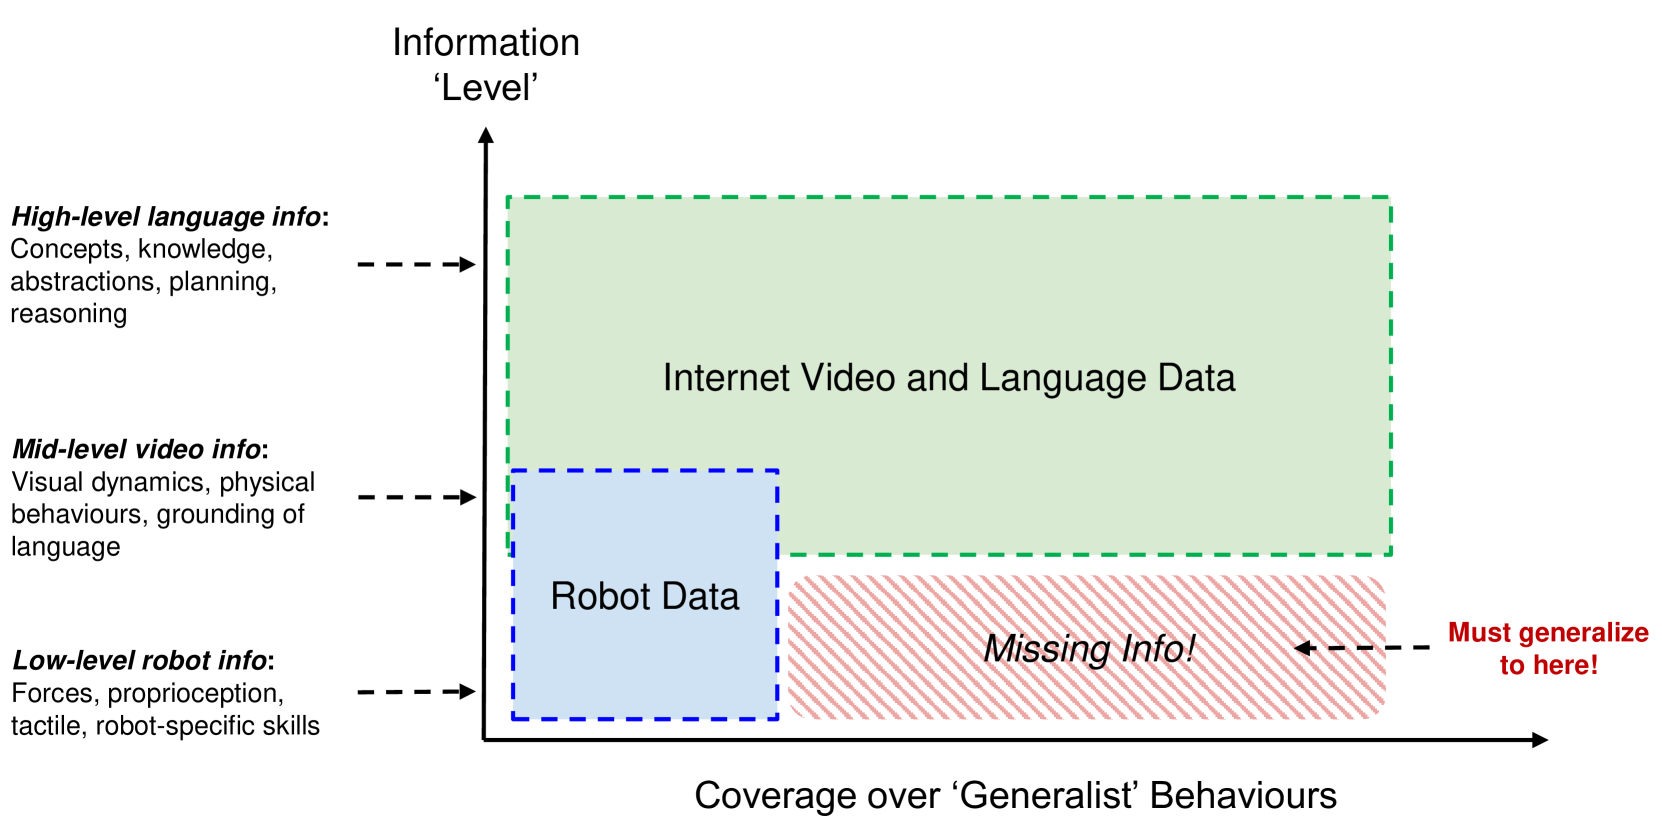
\includegraphics[width=1.0\linewidth]{./chapter4/media/DataBottleneck}
	\caption[Problem: Data Bottleneck in Robotics]{Problem: Data Bottleneck in Robotics. Image source: \cite{McCarthy_2025}.}
	\label{fig:DataBottleneck}
\end{figure}

Figure \ref{fig:DataBottleneck} illustrates the  data bottleneck in robotics. The x-axis represents the spectrum of behaviors that a generalist robot is expected to perform, while the y-axis reflects the different levels of information present in various data sources. The figure highlights that, although internet data encompasses a broader range of behaviors in diverse real-world scenarios compared to specialized robot datasets, it often lacks the detailed, low-level information that is critical for robotic applications.  
Ideally, for every relevant behavior, both low-level robot data and internet data would be available, allowing a model to establish connections across different information levels. However, as illustrated in Figure \ref{fig:DataBottleneck}, there is a significant lack of low-level robot data for many behaviors that are well represented in internet data (see ``Missing Info'' area). 
% This gap in fine-grained information presents a major challenge for learning generalist robotic skills from diverse data sources.
This absence of fine-grained information poses a significant challenge for generalizing robot learning beyond the limitations of available robot datasets \cite{McCarthy_2025}. Overcoming this gap and effectively leveraging both broad internet data and precise robot data is a central objective in advancing \ac{LfV} approaches \cite{McCarthy_2025}.



\textit{Goal of Learning from Videos.} \ac{LfV} aims to exploit this abundance of video data to improve robotic learning. \cite{McCarthy_2025} says, the goal of \ac{LfV} is to leverage our combined \ac{LfV} dataset, $D = \{D_{robot}, D_{video}\}$, to obtain an improved policy $\pi(a_t | s_t)$ versus when learning from $D_{robot}$ alone. 


% While robot datasets provide precise information about robot actions and control, video datasets contain high-level information about how tasks are performed in diverse real-world scenarios. Combining both sources of data can therefore help robotic systems learn beyond the limitations of traditional robot-only datasets.


\paragraph{Improvements of Learning from Videos.} 
What can we expect from combining both data sources, $D_{\text{robot}}$ and $D_{\text{video}}$, instead of using only $D_{\text{robot}}$? 

\begin{itemize}
	\item \texttt{Generalization beyond $D_{\text{robot}}$.}
	One important improvement of \ac{LfV} is the potential to generalize beyond the limited set of tasks contained in the robot dataset $D_{\text{robot}}$ \cite{Eze2024LearningBW}. While robot data primarily provides information about low-level robotic skills, such as grasping or locomotion \cite{Chen2024RH20TPAP}, internet-scale video data contains a much broader variety of tasks and human behaviors. By combining both data sources, models may learn how low-level robot actions relate to higher-level task structures observed in videos. As a result, an \ac{LfV} system may be capable of solving tasks that are not explicitly present in $D_{\text{robot}}$ but are represented within $D_{\text{video}}$ \cite{Brohan2023RT2VM, Du2023LearningUP, Wu2023UnleashingLV, Wang2023MimicPlayLI}.

	\item \texttt{Emergent Capabilities.}
	In natural language processing and computer vision, the availability of large-scale internet data has led to significant improvements and, in some cases, the emergence of capabilities that were not explicitly trained for \cite{Radford2019LanguageMA, Brown2020LanguageMA}. Similar progress is expected in robotics. By combining robot interaction data with internet-scale video data with language annotations, models may learn to connect low-level robotic skills with rich semantic abstractions and higher-level world knowledge obtained from textual data \cite{Achiam2023GPT4TR}. This combination has the potential to improve generalization, task understanding, and the ability to solve previously unseen tasks.

	\item \texttt{Improvements in-distribution of $D_{\text{robot}}$.}
	Furthermore, video data may also improve performance on tasks that are already represented within the robot dataset $D_{\text{robot}}$ . Since robot demonstrations are expensive to collect, additional video data can improve data efficiency and help models learn more robust visual and task representations \cite{Nair2022R3MAU}. As a result, \ac{LfV} approaches may achieve higher task success rates and overall better performance compared to approaches trained solely on robot interaction data \cite{Wu2023UnleashingLV}.
\end{itemize}










\paragraph{Information Levels:}
Robot data primarily contains low-level and mid-level information and can be collected from both real-world and simulation, with real-world data being more valuable. In contrast, internet data is typically richer in mid-level and high-level information. The following sections explain each information level in detail.

\begin{itemize}
	\item \textit{Low-Level Robot Information.} 
	Low-level robot information refers to sensory and control signals that directly describe the robot's physical state, motion, and interaction with its environment. This includes, for instance, end-effector pose, joint positions, joint velocities, joint torques, and gripper state (e.g., open or closed). Additionally, low-level information includes information about the physical forces acting on the robot itself. In simulation environments, they may include physical details of objects in the environment, such as contact forces, object properties or object dynamics.
	Such low-level informations are essential for learning precise motor control tasks, including grasping, locomotion, and manipulation.

	\textbf{Proprioceptive information} refers to the robot's internal sense of its own body and movement. It includes data about the robot's end-effector pose which implicity inlcudes joint angles, joint velocities, and gripper configuration. This information is crucial for executing accurate and stable motions, as it allows the robot to understand its current state and adjust its actions accordingly. 
	A robot may visually observe a cup through a camera and wants to grasp it. Proprioceptive information tells the controller how to move the arm to the cup, which includes:
	\begin{itemize}
		\item what is the current pose/state of the robot
		\item how far the arm has moved,
		\item whether the wrist is rotated correctly,
		\item whether the gripper is aligned with the handle.
	\end{itemize}


	\textbf{Tactile data} refers to information obtained through physical contact between the robot and its environment. It is comparable to the human sense of touch. Common tactile signals include contact forces, pressure distributions, slip detection, surface texture information, and vibration signals. These measurements are typically acquired using sensors placed on robot grippers, fingertips, or other contact surfaces.
	For instance, during grasping, tactile sensors can indicate whether an object has been successfully grasped, whether it is slipping, or whether excessive force is being applied. This feedback is critical for maintaining stable and safe object manipulation.

% This information is essential for tasks that require physical manipulation and interaction with objects, such as grasping, pushing, or opening doors.


% Tactile data refers to information obtained through physical contact with objects or surfaces. It is comparable to the human sense of touch.




% For example, when a robot arm grasps a cup, the robot needs to know the pose of the cup and the robots end-effector and how to move the arm to the cup, which implizity includes information to it's joint angles, joint velocities, and gripper configuration in order to execute stable and accurate movements. 
% This information allows the robot to execute accurate and stable motions.

% Tactile information provides critical feedback about the physical interaction between the robot and its environment, such as contact forces, pressure distributions, slip detection, texture information, and vibration signals. This information is essential for tasks that require physical manipulation and interaction with objects, such as grasping, pushing, or opening doors. Tactile sensing allows the robot to adjust its actions based on the feedback received from the environment, enabling more robust and adaptive behavior during physical interactions. 
% and plays a crucial role in physical interaction.



	\item \textit{Mid-Level Video Information.}
	Mid-level video information refers to visual observations that capture the dynamics of objects, agents, and environments over time without providing explicit low-level control signals. In contrast to robot data, video data does not include direct information about actions or internal robot states, instead it provides sequences of RGB observations that encode how the visual scene evolves over time.

	This type of information includes visual dynamics such as object motion, changes in spatial configurations, and interactions between entities in the scene. For example, videos can capture how objects are moved, grasped, or manipulated by humans, as well as how these actions affect the surrounding environment. Although no explicit force or control signals are available, the physical behavior of objects (e.g., sliding, rotating, or deforming) can often be inferred implicitly from the visual changes across frames.

	A key aspect of mid-level video information is that it encodes \textbf{physical behavior at a perceptual level}. While it does not provide direct measurements of forces or torques, it still reflects underlying physical principles such as gravity, friction, and object permanence through observable motion patterns. For instance, a video of a person pouring water into a glass implicitly contains information about liquid flow dynamics and object interaction constraints.

	In addition, mid-level video information provides a natural source for \textbf{language grounding}. Many video datasets are paired with textual annotations, captions, or narration, which link visual observations to semantic concepts. This allows models to associate language with observed actions and events, such as "opening a door", "placing an object on a table", or "picking up a cup". Through such alignment, video data helps bridge the gap between perception and high-level task understanding, enabling learning of more abstract representations that go beyond purely visual dynamics.


% Mid-level video information refers to the semantic and structural information that can be extracted from video data, which is relevant for understanding and performing tasks. This includes information about object interactions, human behaviors, task execution patterns, and the underlying structure of activities. For example, videos can provide insights into how objects are manipulated, how humans perform tasks, and how different actions are sequenced to achieve a goal.


	\item \textit{High-Level Language Information.}
	High-level language information refers to abstract semantic descriptions of tasks, concepts, and behaviors expressed in natural language. In contrast to visual or robot-centric signals, language does not encode direct sensory observations or motor commands but provides structured knowledge about goals, constraints, and task structures. This includes descriptions of concepts (e.g., objects and their properties), relational knowledge, and symbolic abstractions of actions and environments.

	Such information is particularly important for representing task intent and enabling generalization across different embodiments and environments. Language can describe tasks at multiple levels of abstraction, ranging from low-level action descriptions (e.g., ``pick up the cup'') to high-level procedural or goal-oriented instructions (e.g., ``prepare a table for breakfast''). This hierarchical structure allows models to connect concrete behaviors with more abstract task specifications.


	Language plays a central role in \textbf{planning and reasoning}. It provides a medium for expressing sequential structure, subgoals, and dependencies between actions. For example, a task such as ``clean the table'' can be decomposed into intermediate steps such as removing objects, wiping the surface, and reorganizing items. Such decompositions reflect implicit reasoning about task structure and enable more systematic policy learning.

	Furthermore, language serves as a bridge for incorporating prior knowledge into robotic systems. Through textual descriptions, models can access commonsense knowledge about object affordances, physical interactions, and typical human behaviors. This enables improved generalization to unseen tasks by leveraging semantic relationships that are not explicitly present in robot or video data alone.
\end{itemize}


% The objective of Learning from Videos (LfV) is to utilize the combined dataset
% \begin{equation}
% D = \{D_{\text{robot}}, D_{\text{video}}\}
% \end{equation}
% to learn a policy $\pi(a_t \mid s_t)$ that achieves better generalization and task performance compared to training solely on robot interaction data $D_{\text{robot}}$.


	
	
	% of large-scale internet video data, which provides rich information about human behaviors, object interactions, and task execution in diverse environments.

\section{Challenges of Video Data} \label{sec:ChallengesOfVideoData}






% A key advantage of video-based instructions is that they naturally capture complex, multi-step behaviors and temporal dependencies. However, they also introduce challenges such as high data requirements, sensitivity to visual variations, and the need to extract relevant features from long and potentially noisy observation sequences.

Although internet-scale video data offers significant potential for robotic learning, it also introduces several fundamental challenges, see Figure \ref{fig:KeyChallengesInLfV}. 
In contrast to robot interaction datasets, videos are typically high-dimensional, noisy, weakly labeled, highly diverse and lacks on low-level information. Extracting meaningful representations and task-relevant information from such data is therefore a non-trivial problem \cite{McCarthy_2025}.


\begin{figure}[!ht]
	\centering
	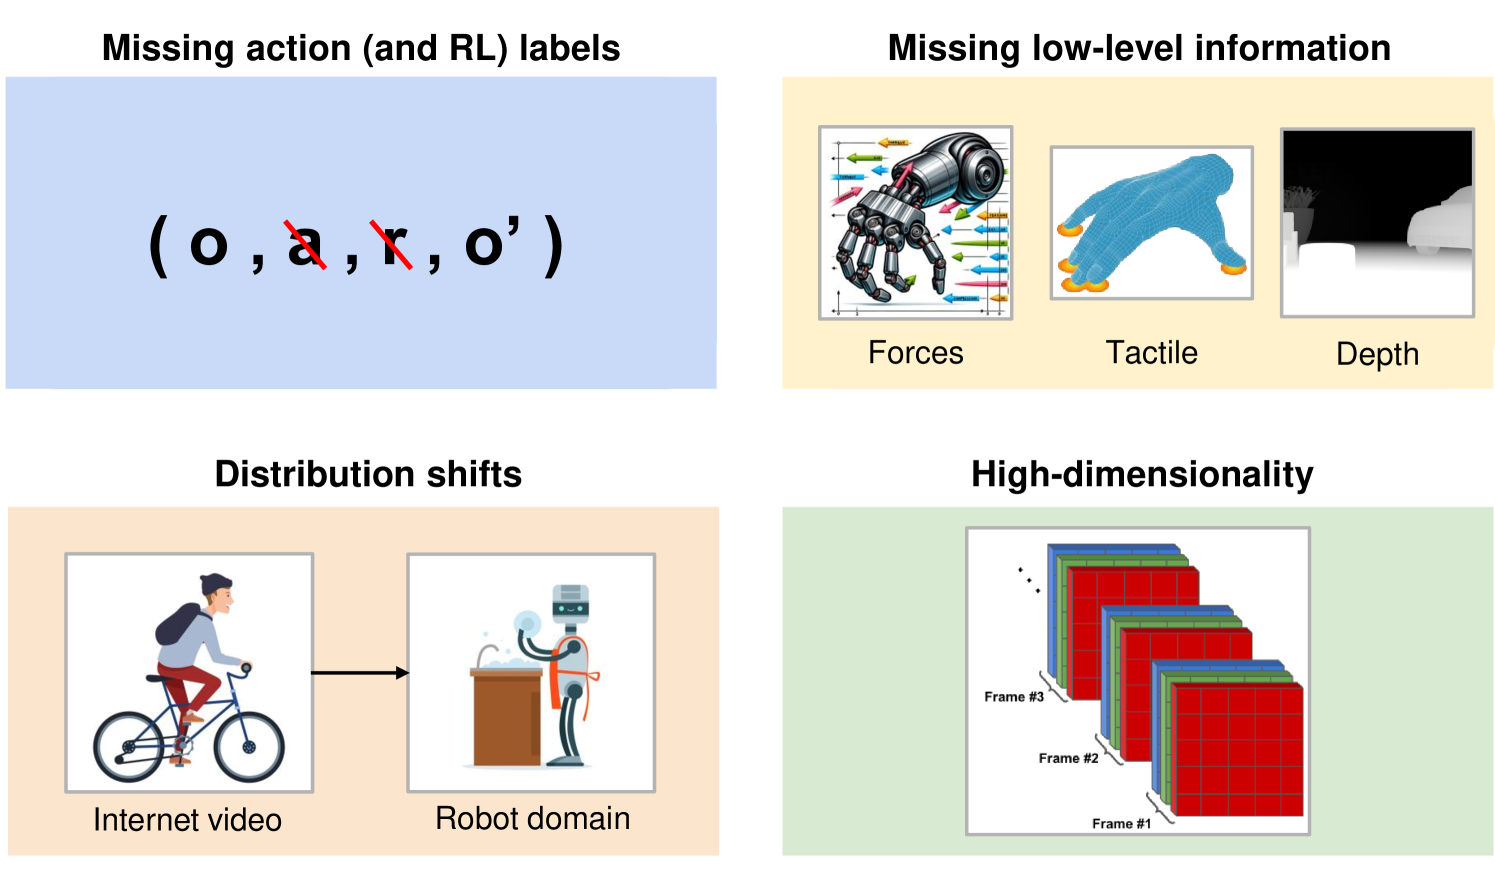
\includegraphics[width=1.0\linewidth]{./chapter4/media/KeyChallengesInLfV}
	\caption[Key Challenges in \acs{LfV}]{Key challenges in Learning from Videos. Image source: \cite{McCarthy_2025}.}
	\label{fig:KeyChallengesInLfV}
\end{figure}

\paragraph{Missing Action Labels}
One major limitation of raw video data is the absence of explicit action labels required by many \ac{IL} \cite{Brohan2022RT1RT} and offline \ac{RL} approaches \cite{Chebotar2023QTransformerSO}. While videos provide rich visual observations of behaviors, they typically do not contain the low-level control commands executed during the task. Retrospectively inferring robot actions from human videos is challenging, since human motions often cannot be directly mapped to the action space of a robotic system. Furthermore, videos usually lacks on \ac{RL} signals such as reward annotations, goal labels, or start-of- and end-of-episode boundaries \cite{McCarthy_2025}.


\paragraph{Missing Low-level Information}
Internet videos also lack on low-level sensory information. Skillful behaviors often depend on tactile feedback, force measurements, proprioceptive signals, or depth information, which are generally not observable in classical RGB videos. Although videos may capture high-level task structure and object interactions, they do not explicitly provide the fine-grained physical information necessary for learning accurate motor control and stable interaction with the environment \cite{McCarthy_2025}.


\paragraph{Distribution Shift}
Another challenge arises from the distribution shift between internet videos and the downstream robotics domain. Differences may occur in camera viewpoints, environments, embodiments, object appearances, and task distributions. The Human demonstrations in videos may contain behaviors that are inefficient, ambiguous, or irrelevant for robotic execution \cite{McCarthy_2025}.

In particular, \ac{LfV} must address the embodiment gap between humans and robots as they often differ significantly in their kinematics, morphology, and control capabilities. Furthermore, there exists a visual gap between the human actor performing the task in the video and the robotic embodiment that is expected to execute the task. As a result, transferring observed human motions directly to robot actions is highly non-trivial and requires models to learn embodiment-invariant task representations \cite{McCarthy_2025}.

Additionally, some important robotic tasks, such as specialized industrial manipulation tasks, may be difficult to learn because they are underrepresented in publicly available video datasets \cite{McCarthy_2025}.

\paragraph{High-dimensionality, Noise, and Redundancy}
Video data is inherently high-dimensional and often contains substantial amounts of irrelevant or redundant information. Background changes, camera motion, occlusions, and unrelated actions can make it difficult for models to identify task-relevant features, making it challenging to learn robust representations. Furthermore, the sheer volume of video data can lead to computational challenges in processing and learning from such large datasets \cite{bardes2024vjepa}.


\paragraph{Controllability, Stochasticity, and Partial Observability}
In unlabeled video data, it can be tricky for models to determine which changes in the environment are caused by the agent's actions and which originate from external factors or environmental noise \cite{Horan2021WhenIU}. This ambiguity makes it challenging to infer action information directly from video observations. Furthermore, real-world environments are frequently stochastic and only partially observable, meaning that important state information may be hidden from the camera viewpoint \cite{Babaeizadeh2017StochasticVV}. As a result, predicting future states or accurately modeling action consequences from video alone becomes a difficult problem.


\paragraph{Summary}
None of these challenges have yet been fully solved. In the following sections, we will discuss some possible ways to address these issues coming with internet video data. Nevertheless it seems likely that scaling — with the help of internet video data — can provide significant gains in robotic systems within the near future \cite{McCarthy_2025}.



% Existing LfV research has shown promising signs of life, and this is a field ripe for further progress. Of course,
% it is unclear whether scaling deep learning will take us all the way to general-purpose robots (Section 6.4), and
% there are other research directions that should be pursued in parallel (Section 2). Nevertheless, with sufficient
% effort and innovation, it seems likely that scaling—with the help of internet video data—can provide significant
% gains in the near-future



% **Missing Action Labels**

% - **video** lacks **information** critical to robotics, including action labels and low-level force and proprioceptive information

% **Missing Low-level Information**

% - For certain skillful behaviours, robots require low-level percepts such as tactile sensing, forces, proprioception, or depth sensing
%     - data not explicitly available in internet video.

% **Distribution-shift**

% - various distribution shifts between internet video and the robot domain.
% - shifts between an internet video dataset and the downstream robot domain.
%     - physical embodiments, camera viewpoints, tasks, and environments
% - Humans in videos may perform behaviours which are sub-optimal or irrelevant
% - useful tasks and behaviours may be underrepresented in internet video
% - **embodiments** from robots very **different from that of a human may prove more effective**

% **High-dimensionality, Noise, and Redundancy**

% - challenging to extract meaningful information and representations from video data
% - some important actions and tasks may be underrepresented in the video dataset
%     - e.g., specialized industrial tasks
%     - the robot may need to perform tasks not commonly performed by humans


% \subsection{Other Paths to Generalist Robots.}


% Goal: reduce the amount of robot videos

% - **Video provides foundational information:**
%     - Contains physics and dynamics information
%     - Shows human behaviors, tasks and actions relevant to robots
%     - High quantity and diversity
%     - Relatively untapped resource
%     - —>can be highly informative for general-purpose robots.
% use of diverse internet data has facilitated a transition from task-specific models to monolithic foundation models with more general capabilities


% \ac{LfV} will solve the data bottleneck by augmenting traditional robot data with large-scale internet video.















% \ac{IL} (IL) is a powerful approach for training agents to perform complex tasks by learning from demonstrations provided by an expert. The main advantage of IL is that it can leverage large datasets of human demonstrations, which are often easier to collect than reward signals. This allows IL to learn complex behaviors that are difficult to specify with a reward function, and can be more sample efficient than reinforcement learning, especially in high-dimensional state spaces.





% —> learning a KM from a video dataset and finetune it to the robot domain

% Different approaches to transfer the knowledge

% - **Generalisation and zero-shot transfer:**
% pretrained KM directly in the target setting, without further fine-tuning or adaptation
% - **Fine-tuning and Representation transfer:** 
% methods that train a model in the robot domain that is partially composed of parts of a pretrained KM
% - **Hierarchy: conditioning**
% involves using a pretrained KM to condition a new KM being trained in the target MDP




%  In-the-wild videos are particularly valuable for training robots to operate in diverse and unstructured environments, as they capture a wide range of scenarios, object appearances, lighting conditions, and background variations that the robot may encounter in real-world applications. However, learning from in-the-wild videos also introduces significant challenges, such as dealing with noisy data, occlusions, varying viewpoints, and the need for robust feature extraction to identify relevant information for task execution. Despite these challenges, leveraging in-the-wild videos can significantly enhance the generalization capabilities of robotic systems and enable them to perform effectively in real-world settings.

  

\chapter{Ways to Instruct Robots}
\label{chap:WaysToInstructRobots}
\minitoc
This chapter discusses the various ways in which the robot can be taught its task and how the interaction between humans and robots can be designed.
 
% \texttt{Intend task from scene}
\section{Scene Understanding}

The robot derives its task solely from the environment and the objects present in it and is not explicitly conditioned \cite{jang_BCZZeroShotTask_2022}. For example, if a teapot and a cup are present, the robot may infer that the task is to pour liquid from the teapot into the cup. This approach relies heavily on the robot's ability to understand the scene based on visual cues \cite{jang_BCZZeroShotTask_2022}.
% and infer the intended task based on visual cues and contextual information \cite{jang_BCZZeroShotTask_2022}. 
A distinction can be made between a policy that can identify and execute multiple tasks and a policy that can handle only a single task.

\paragraph{One Policy, Multiple Tasks}
In this setting, a single policy is typically specialized on a finite set of tasks. The policy must be explicitly trained for those tasks and tasks that are not represented or underrepresented in the training dataset, can therefore often not be executed reliably \cite{_BoostingRoboticManipulation_, mandi_CACTIFrameworkScalable_2023}. For example, if the policy has been trained on multiple manipulation tasks and one of them involves pouring liquid from a teapot into a cup, the policy will execute this behavior when a matching scene is observed during inference \cite{jang_BCZZeroShotTask_2022}.
However, generalization to other objects or situations is often limited. Using different teapots or cups may not be problematic as long as the relevant visual features are recognized. In contrast, performance typically decreases under significantly different objects or scenes \cite{jang_BCZZeroShotTask_2022}. 
% If a corresponding pouring behavior from a cooking pot was not included during training, the policy may fail to transfer the action to that new object category \cite{_BoostingRoboticManipulation_, jang_BCZZeroShotTask_2022}.
A major limitation of this approach is task ambiguity caused by overlapping object context across different behaviors. If the same object types, such as a teapot and a cup, appear in both a pick-and-place task and a pouring task, the policy may not be able to disambiguate the correct action target based on scene context alone \cite{tamar_IMITATIONLEARNINGVISUAL_2018}.


\paragraph{One Policy, One Task}
An alternative approach is to train a separate policy for each individual task, which is then selected explicitly during inference. 
The task-specific policy selection can be performed either manually by a human or automatically by a separate \ac{AI} classification model that analyzes the scene and determines the appropriate policy \cite{chen_RoboRouterTrainingFreePolicy_2026}. For example, one policy could be trained for ``pouring'', another for ``opening a drawer''. This modular design is closely related to task-aware expert routing and decoupled planning-and-execution frameworks in robotic manipulation \cite{chen_RoboRouterTrainingFreePolicy_2026}.
This decoupling enables training each policy on significantly larger and more diverse datasets containing varied object appearances and environmental conditions, while keeping the core task semantics fixed \cite{raffin_DECOUPLINGFEATUREEXTRACTION_2019}. Consequently, these specialized policies often support more robust generalization across novel object instances and environmental variations compared to the \textit{One Policy, Multiple Tasks} paradigm. \cite{bai_LearningSeeAct_2025, _MultitaskRobotManipulation_a, tamar_IMITATIONLEARNINGVISUAL_2018}





\section{Language Instructions}

For humans, the most comfortable way to instruct the robot is with voice commands. This is very useful for simple tasks that are easy to summarize. But complex tasks, where execution must follow exact instructions, are sometimes difficult to describe in words \cite{Jain2024Vid2RobotEV}. For example, how would you teach a humanoid robot to decorate tables exactly like a sample table, especially when various decorations need to be assembled in a complex arrangement?
Furthermore ambiguities may arise, and the same instruction may be interpreted differently according to the linguistic context. For example, the word ``open'' is used for: open drawer, open cabinet, open container with lid or open jar with screw cap. Although the same verb is used here, each interaction requires a completely different motor control \cite{Jain2024Vid2RobotEV}.
Commanding the robot with voice commands enables an interactive dialogue between humans and the robot. If the robot does not understand the instructions, it can ask follow-up questions to clarify any misunderstandings. This helps minimize the problems associated with voice commands.



\section{Image Instructions}

Robots can also be instructed using visual inputs such as images. Compared to language, image-based instructions provide a more concrete and unambiguous specification of spatial arrangements, object relations and desired outcomes.

A common approach is the use of \textbf{goal images}, where the robot is given a visual representation of the desired final state. The robot observes the current state and acts such that it minimizes the difference to the goal image. This is often referred to as goal-conditioned behavior. However, this approach does not explicitly specify \textit{how} the task should be executed, only \textit{what} the final configuration should look like. But some works have addressed this issue with the usage of annotations in the image of the initial state to specify the task execution. For example \cite{bai_LearningSeeAct_2025} highlights the relevant objects and regions with circles and arrows to visualize the task execution in the image, see \autoref{fig:ImageInstructions}. 
Another way to address this limitation, \textbf{subgoal images} or intermediate states can be provided \cite{pathak_ZeroShotVisualImitation_2018}. These guide the robot through a sequence of visually defined steps, effectively decomposing complex tasks into simpler stages. This is particularly useful for long-horizon or multi-step manipulation tasks.

\begin{figure}[h]
	\centering
	\subfigure[Task: Rotate cup and place it on table]{
		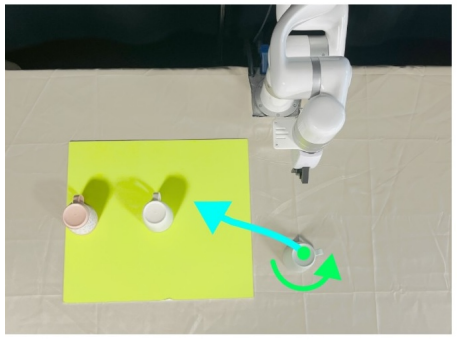
\includegraphics[width=4.5cm]{./chapter4/media/ImageInstruction_1}
		\label{fig:ImageInstruction_1}
	}
	\hspace{0.5cm}
	\subfigure[Task: Put fruit into bowl]{
		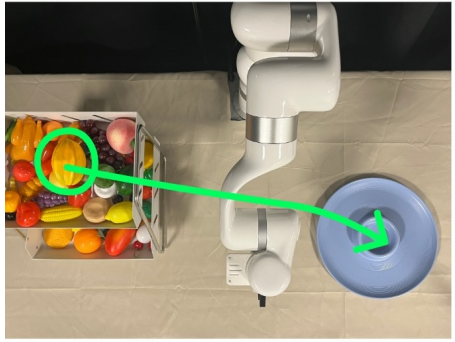
\includegraphics[width=4.5cm]{./chapter4/media/ImageInstruction_2}
		\label{fig:ImageInstruction_2}
	}
	\hspace{0.5cm}
	\subfigure[Task: Fold T-shirt]{
		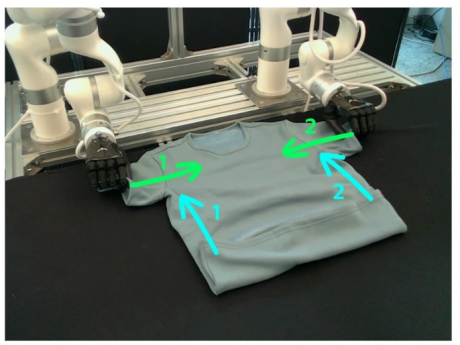
\includegraphics[width=4.5cm]{./chapter4/media/ImageInstruction_3}
		\label{fig:ImageInstruction_3}
	}
	\caption[Image-based instructions for task execution.]{Image-based instructions for task execution: Highlighting relevant objects and regions with circles and arrows to visualize the task execution. Image source: \cite{bai_LearningSeeAct_2025}.}
    \label{fig:ImageInstructions}
\end{figure}

A key advantage of image instructions is their ability to capture fine-grained spatial details that are difficult to describe in language, such as precise object placement, orientation or symmetry alignments. However, they also introduce challenges related to perception, such as viewpoint variation, occlusions of objects in the real environment, or the use of in-the-wild goal-images with varying lighting and background conditions.




\section{Video-Based Instructions}

Demonstration videos are a powerful way to instruct robots, as they contain rich visual and temporal information. In contrast to single images, videos provide not only the desired goal state of a task but also the sequence of intermediate steps required to reach that goal \cite{Jain2024Vid2RobotEV}.
In this setting, the task is typically formulated as an \ac{IL} problem, where the robot learns a policy that maps visual observations to actions by imitating the demonstrated trajectory \cite{Jain2024Vid2RobotEV}. The temporal structure of the video enables the robot to infer \textit{how} a task should be executed, rather than only \textit{what} the final outcome should look like. Depending on the setup, this may also require inferring latent actions from visual observations alone \cite{Jain2024Vid2RobotEV}.
Ideally, the robot model should be able to understand it's task from in-the-wild demonstration videos of both robots and humans \cite{Chen2025VidBotLG}. Such data exhibits large variability in lighting, backgrounds, and camera motion, making it significantly more challenging for perception and learning compared to controlled laboratory data.
% In-the-wild videos refer to video data collected in unconstrained, real-world environments, without controlled settings, standardized viewpoints, or curated conditions.

Demonstration videos from humans and robots differ in their characteristics and are challenging for learning. In addition, a third category ``teleoperation'' is being introduced, which is often used for fine-tuning the robot. There a human directly controls the robot to generate demonstrations.
The following sections discuss the specific advantages and challenges of each type of demonstration video.

\paragraph{Human Video Demonstrations}
Human demonstrations videos are a natural and intuitive way to teach robots.  However, these videos are commonly Raw RGB or RGB-D videos with depth, which lack explicit on action labels and trajectory data. 
The characteristics of human demonstration videos are:
\begin{itemize}
	% In this paradigm, the robot learns from videos of humans performing a task. This is particularly appealing, as l
	\item \textbf{Data Abundance:} Large amounts of human demonstration data are readily available on the internet \cite{McCarthy_2025, Eze2024LearningBW}. 
	\item \textbf{Embodiment Gap:} A core challenge is the mismatch between human and robot bodies. Human motions and kinematics differ significantly from those of robots and the robot must learn to map observed human actions to its own action space \cite{McCarthy_2025}.
	\item \textbf{Suboptimal Demonstrations:} Another key challenge of human video demonstrations is that they do not necessarily represent optimal task executions. Demonstrations often reflect individual preferences, inefficiencies, or context-specific behaviors, resulting in suboptimal trajectories. In many cases, a video captures only a single possible way of solving the task without providing information about alternative or more efficient strategies. However, the objective for the robot is typically to perform tasks efficiently and robustly. Therefore, the learned policy must be able to generalize beyond the demonstrated behavior and, if necessary, improve upon it, rather than directly imitating potentially suboptimal actions \cite{McCarthy_2025}.
\end{itemize}






\paragraph{Robot Video Demonstrations With No Trajectory Information}
RGB and RGB-D robot demonstration videos lack, like human videos on action labels and trajectory data too, but with the difference that the robot is performing the demonstration. These videos are recorded from the robot's perspective or a stationary camera. This also includes demonstrations in which a person operates with a robotic arm in their hand or holds a robotic gripper to perform tasks. The characteristics of robot demonstrations videos are:
\begin{itemize}
	\item \textbf{No Embodiment Gap:} The demonstrations are performed by the robot itself or by another robot with similar embodiment. This avoids the human-robot embodiment gap and provides more directly transferable data \cite{McCarthy_2025}. 
	\item \textbf{Cost and Effort:} Collecting robot demonstrations is often expensive and time-consuming, as it requires access to robotic systems and typically controlled environments. In addition, purely visual robot demonstrations may still lack explicit action labels. This means that the robot must still infer the underlying actions and intentions from the visual data \cite{McCarthy_2025}. 
	\item \textbf{Value of Robot Demos:} Despite these challenges, robot video demonstrations can provide valuable data for learning, as they are more closely aligned with the robot's own capabilities and constraints compared to human demonstrations \cite{McCarthy_2025}.
\end{itemize}



\paragraph{Teleoperation}
Teleoperation videos contain not only visual observations but also trajectory and action information. 
The demonstrations are generated by directly controlling the robot, e.g. via a joystick or a dedicated control interface \cite{McCarthy_2025}.
%  and all trajectory information are recorded \cite{McCarthy_2025}.
\begin{itemize}
	% \item \textbf{Direct Data Collection:} A common method to generate high-quality robot demonstrations is teleoperation, where a human operator directly controls the robot, e.g. via a joystick or a dedicated control interface \cite{McCarthy_2025}.
	\item \textbf{Precision and Safety:} 
	% In contrast to passive video demonstrations, teleoperation provides access to both the visual observations and the corresponding action and trajectory data. As a result, 
	The demonstrated actions are already expressed in the robot's action space, which significantly simplifies reproducing the expected behavior. Such demonstrations are particularly important for fine-grained manipulation tasks that require precise control and accurate timing  \cite{McCarthy_2025}. 
	\item \textbf{Scalability Issues:} However, teleoperation may require specialized hardware (controllers, sometimes motion-capture or VR setups) and does not scale as easily as collecting passive video data. Thus, collecting large teleoperation datasets can be time-consuming and is typically done in lab settings only \cite{McCarthy_2025}.
\end{itemize}


  % What is model based control?
% Video to text vs. Video language models?
\chapter{Learning from Videos - Data Modality and Challenges}

Videos are a challenging data modality, as you have seen in Section~\ref{sec:ChallengesOfVideoData}. This section addresses the two key questions for \ac{LfV} research:
\begin{enumerate}
    \item How to extract relevant knowledge from internet video?
    % \item How to apply video-extracted knowledge to robotics?
    \item How to apply video-extracted knowledge to robotic systems for policy learning and control?
\end{enumerate}
We first review different approaches for extracting foundational knowledge from internet video, including video encoders, video prediction models, and video-to-text models. We then discuss methods for transferring video-extracted knowledge to robotics, addressing challenges such as missing action labels and distribution shift. 

% it is high-dimensional, noisy, and poorly labelled. Second, video lacks information critical to robotics, including action labels and low-level force and proprioceptive information. Moreover, there may be various distribution shifts between internet video and the robot domain.


\section{Extracting Foundational Knowledge from Internet Video} 
\label{sec:ExtractingFoundationalKnowledgeFromInternetVideo}

% The Answer to the first question of how to extract relevant knowledge from internet video is may be using techniques and datasets inspired by video foundation Models (FMs).

Recent progress in \textbf{Video \acp{FM}} provides a promising direction for addressing the first answer: How to extract robotic relevant knowledge from internet video. Video \acp{FM} are large-scale deep learning models trained on massive internet video datasets. Through large-scale training, these models learn general visual and temporal representations that capture semantics, motion dynamics, physical interactions and behavioral patterns. As a result, they can extract foundational knowledge that is transferable across a wide range of downstream tasks, including robotics applications \cite{Madan2024FoundationMF}.

\begin{samepage}
McCarthy et al. \cite{McCarthy_2025} says, Video \acp{FM} can be highly applicable for the following \ac{LfV} use-cases, see Figure \ref{fig:VideoFoundationModellingForLfV}:
\begin{itemize}
    \item \texttt{Finetune Pretrained Video \acp{FM}:} 
    One important application of Video \acp{FM} is the transfer of pretrained models to robotics tasks. For example, a video prediction model trained on internet video data may be adapted or fine-tuned into a robot dynamics model, allowing the robot to leverage the broad gathered knowledge about object motion and environmental dynamics from the pretrained Video \acp{FM} \cite{Yang2023LearningIR, rt22023arxiv, Ahn2022DoAI, Kim2024OpenVLAAO}. 
    
    \item \texttt{Leveraging Techniques and Datasets Inspired by Video \acp{FM}:}
    In addition, techniques developed for video foundation models can be integrated into robot learning pipelines and can lead to better extraction of representations and knowledge. This, in turn, can lead to improved generalization and task understanding. For instance, a Robot \ac{FM} can be directly trained by combining robot data with large-scale video inspired by video \acp{FM} techniques \cite{Team2024OctoAO, rt12022arxiv}.
\end{itemize}
\end{samepage}

\begin{figure}
	\centering
	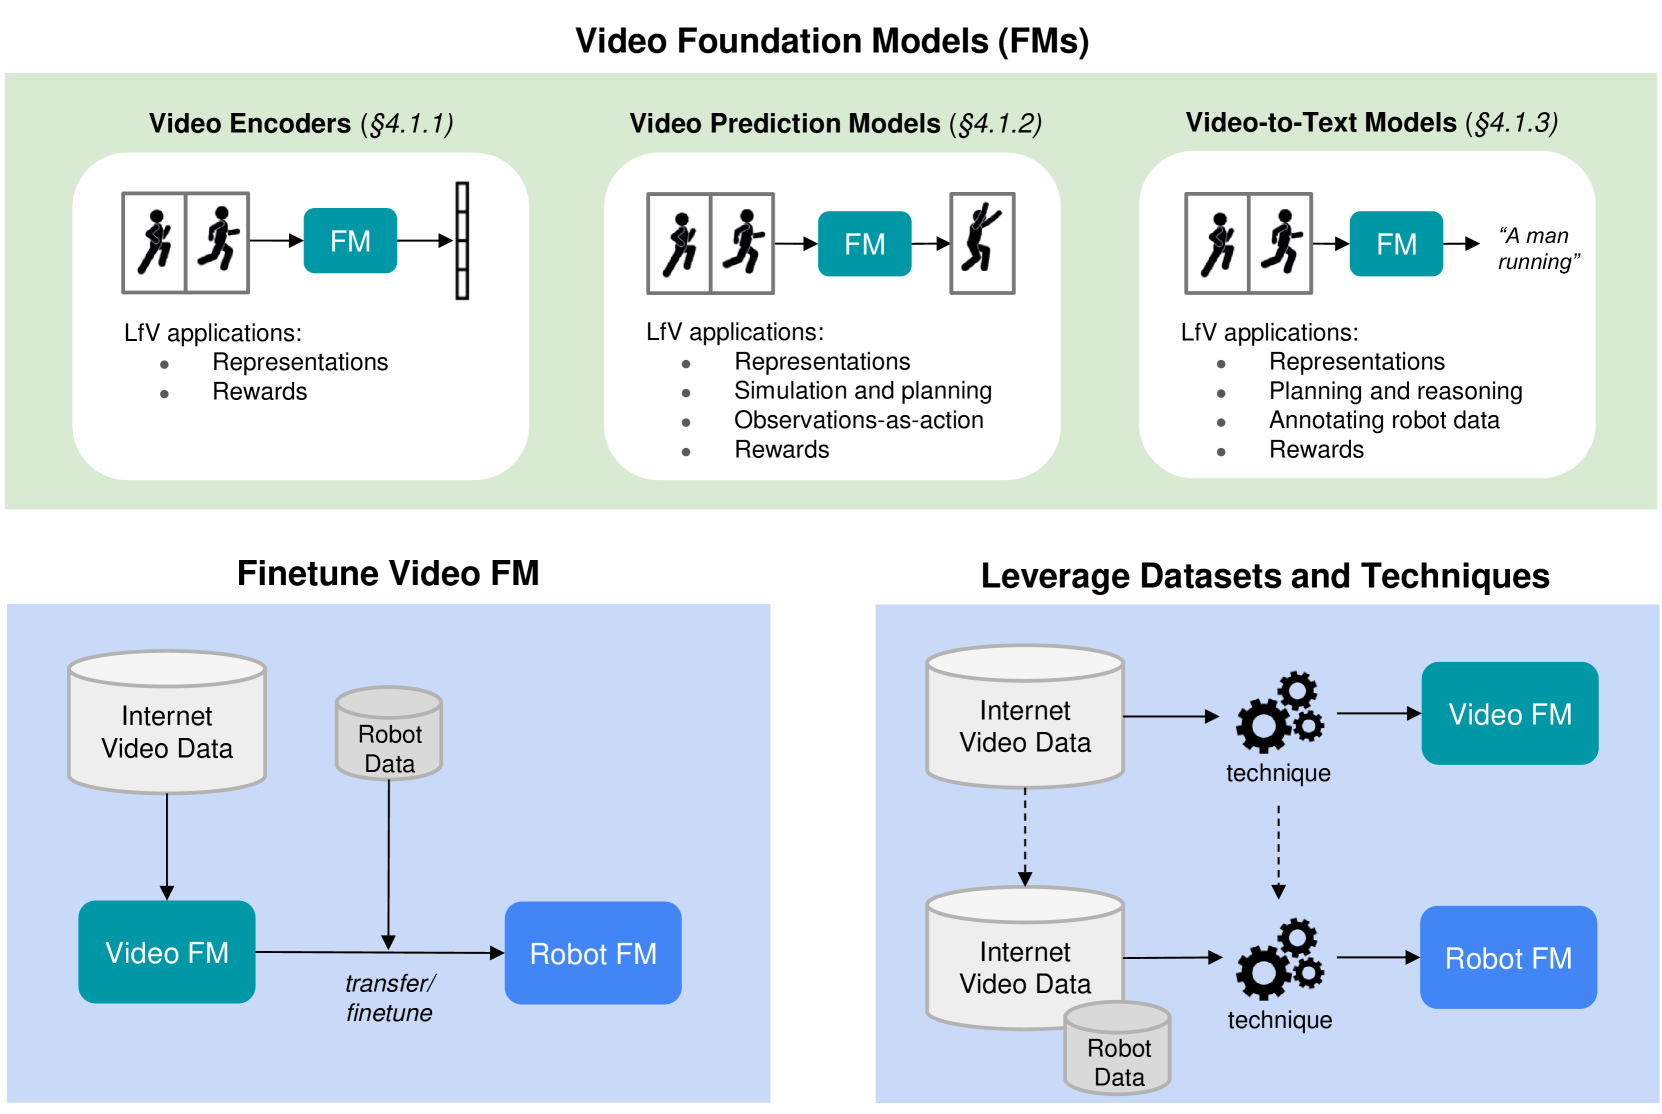
\includegraphics[width=1.0\linewidth]{./chapter5/media/VideoFoundationModellingForLfV}
	\caption[Video Foundation Modelling for LfV]{Video foundation modelling for Learning from Videos. Image source: \cite{McCarthy_2025}.}
	\label{fig:VideoFoundationModellingForLfV}
\end{figure}

% Furthermore, these models can serve as strong initialization policies for \ac{RL}. A common strategy is to first pretrain the model using supervised sequence prediction on large-scale multimodal datasets, and subsequently fine-tune the policy using \ac{RL} with task-specific rewards. This often improves sample efficiency and generalization compared to training \ac{RL} policies from scratch.
% Even when the action prediction head is discarded, the learned encoder can still provide transferable cross-modal representations for downstream robotic tasks. 


\subsection{Video Encoders}
\label{sec:VideoEncoder}
Foundational video encoders are capable of extracting rich and robust representations from raw video observations:
\begin{equation}
    p(z \mid \tau)
\end{equation}
Given a video clip $\tau$, the encoder maps the visual input into a latent representation $z$, which captures semantic and temporal information relevant for downstream robotic tasks.

\paragraph{Relevance for Robotics.}
In robotic \ac{IL}, pretrained video encoders are commonly used in two ways \cite{McCarthy_2025}:
\begin{itemize}
    \item \texttt{Representation Learning:}
    Pretrained video encoders can be transferred to robotic learning frameworks and further fine-tuned on robot-specific data for downstream tasks such as policy learning or an \ac{RL} \ac{KM}. The learned latent representations provide compact and informative features that improve generalization and sample efficiency, by allowing the model to learn task-specific features while still leveraging the general knowledge captured from internet video
    % ToDo: , see Section~\ref{} and maybe some references.
    
    \item \texttt{Reward Learning:} 
    Frozen video representations can also be used to define reward functions for robotic agents \cite{Nair2022R3MAU, Sontakke2023RoboCLIPOD, Fan2022MineDojoBO}. By comparing the latent representations of demonstrations and robot executions, the system can measure behavioral similarity without requiring manually engineered reward signals. This approach enables the robot to learn from video demonstrations by optimizing its behavior to match the latent representations of successful demonstrations, thus facilitating \ac{IL} and skill acquisition.
    % ToDo: , see Section~\ref{}.
\end{itemize}

\subsubsection{Methods}
\paragraph{Video Representation Learning}
Video representation learning aims to learn meaningful latent representations from raw video data. These representations capture semantic, spatial and temporal information that can be used for various downstream tasks \cite{McCarthy_2025}.

Let
\begin{itemize}
    \item $X$ denote a video clip
    \item $\bar X$ denote a video clip paired with some corresponding labels (bounding boxes and object masks \cite{Ding2023MOSEAN}) and data modalities (language annotations \cite{Grauman2021Ego4DAT}, meta-data \cite{ChantrySchiappa2022SelfSupervisedLF})
    \item $Y$ denote a learning objective, derived from $\bar X$
\end{itemize}
\texttt{Learning Goal During Training:} predict $Y$ from $X$.
Or in other words, learn a video encoder $p(z|X)$ that maps the video clip $X$ to a latent representation $z$ that can be used to predict $Y$: $X \xrightarrow{p(z|X)} z \rightarrow Y$ \cite{McCarthy_2025}.
% The objective of the video encoder $p(z|X)$ is then to learn representations $z$ that enable the prediction or alignment of $Y$ from the input video $X$.
% During training, the objective is to learn representations $z$ that enable the prediction or alignment of $Y$ from the input video $X$.
Basic techniques for learning $Y$ include:
\begin{itemize}
    \item \textbf{Prediction-Based Objectives}: The target $Y$, which is derived from the annotated video clip $\bar X$, may correspond to future video frames, masked regions, motion information, or other supervision signals. For example, in video prediction tasks, the model predicts the next frame $x_{t+1}$ from the raw previous observations $x_{\leq t}$ \cite{Gao2022SimVPSY, Jang2024VisualRL}. 
    % The Encoder is optimized using a prediction loss that encourages the learned representation to capture temporal structure and motion dynamics in video sequences.
    % The encoder is optimized using a prediction loss of the form
    % \begin{equation}
    % \mathcal{L}_{\text{pred}} = \| \hat{Y} - Y \|^2
    % \end{equation}
    % where $\hat{Y}$ denotes the predicted target. 
    % Such objectives encourage the learned representation to capture temporal structure and motion dynamics in video sequences.

    \item \textbf{Joint-Embedding Objectives}: Joint-embedding approaches \cite{Oord2018RepresentationLW, Xian2023TowardsGR, bardes2023v} first map both the video input $X$ and the known target $Y$ into a shared latent embedding space:
    \begin{equation}
    z_X = f(X),
    \qquad
    z_Y = g(Y)
    \end{equation}

    A loss function is then applied to align semantically similar embeddings: 
    \begin{equation}
    \mathcal{L}_{\text{pred}} = L_{\text{align}}(z_X, z_Y)
    \end{equation}
    Contrastive learning is one of the most widely used approaches in this setting \cite{ChantrySchiappa2022SelfSupervisedLF}. 
    % These approaches have become highly effective for learning transferable video representations from large-scale unlabeled video datasets.
\end{itemize}


\paragraph{State-of-the-Art Approaches}
Recent work has proposed scalable methods for learning rich spatio-temporal video representations. 
\textit{Video-Text Objectives:} Video-text objectives leverage language annotations to learn semantic representations from video data. Common approaches include:
\begin{itemize}
    \item \textbf{Video-Text Contrastive Learning:} This approaches learn to align video representations with corresponding text descriptions. By maximizing the similarity between video and text embeddings, the model captures semantic relationships between visual content and language \cite{Xu2021VideoCLIPCP, Zhao2024VideoPrismAF, Wang2023InternVidAL, Papalampidi2023ASR, Li2023UnmaskedTT}.
    
    \item \textbf{Video-Text Matching:} This methods train the model to determine whether a given video clip and text description correspond to each other. The model learns to distinguish between matching and non-matching pairs, which encourages it to capture relevant features for both modalities \cite{Li2023UnmaskedTT}.

    \item \textbf{Masked Language Modelling:} In this approaches, the model learns to predict masked words in a text description based on the corresponding video content. This encourages the model to learn contextual relationships between visual information and language \cite{Li2023UnmaskedTT}.

    % ToDo: steht als Video-to-text losses in McCarthy2025 --> ist das hier so richtig
    \item \textbf{Video-to-Text Generation:} This method trains the model to generate descriptive text based on video input. By learning to produce coherent and relevant descriptions, the model captures high-level semantic information from the video data \cite{Papalampidi2023ASR, Yan2022VideoCoCaVM}.
\end{itemize}


\textit{Auto-Encoding Approaches.} Auto-encoding approaches have also become highly effective for self-supervised video representation learning. Auto-encoding approaches learn video representations by reconstructing input data from compressed latent representations. Common approaches include:
\begin{itemize}
    \item \textbf{\ac{MAE}:} In this approach, parts of the video input are randomly masked, and the model is trained to reconstruct the missing regions from the visible observations. This encourages the encoder to learn meaningful spatial and temporal representations from incomplete video information \cite{Wang2023VideoMAEVS, Tong2022VideoMAEMA, Girdhar2022OmniMAESM}.
    % This method learns to reconstruct masked regions of video input, encouraging the model to capture meaningful spatio-temporal structure and context from incomplete observations.
    
    \item \textbf{\ac{VQ-AE}:} 
    In this approach, the encoder first extracts continuous latent features from the video input. 
    These features are then quantized by mapping them to the nearest vector in a finite set of learned codebook embeddings/vectors. 
    The decoder reconstructs the original video from these vector, encouraging the model to learn compact and semantically meaningful representations, due to the limited set of learned embeddings. 
    The underlying principle is similar to language modelling, where a finite vocabulary of discrete tokens is used to represent words, syllables or letters. Analogously, \ac{VQ-AE} learns a finite set of discrete visual tokens that capture recurring patterns in video data. These tokens may represent object appearances, motion patterns, textures, actions, or scene structures \cite{Bruce2024GenieGI, Villegas2022PhenakiVL, Yu2022MAGVITMG, Yan2021VideoGPTVG, Seo2022HARPAL}. 
    % By reusing a limited set of learned embeddings, the model can construct compact and semantically meaningful representations of complex visual observations.
\end{itemize}

\textit{Student-Teacher Distillation Approaches.} Student-teacher distillation approaches learn representations by transferring knowledge from a pretrained teacher network to a smaller student model \cite{Zhao2024VideoPrismAF, Wang2022MaskedVD, Li2023UnmaskedTT}. The student is trained to match the representations or predictions generated by the teacher model. This encourages the student network to learn robust and generalized video representations while often requiring fewer computational resources.

% \item \textbf{Student-Teacher Distillation:} These methods train a student network to match the representations of a pretrained teacher model, transferring knowledge and improving generalization.

\texttt{Joint-Embedding Predictive Architectures (JEPA)} learn representations by predicting high-level latent embeddings instead of reconstructing raw video pixels. Rather than modeling every visual detail, the model predicts semantic representations of future or masked observations in a shared embedding space. This approach improves robustness against the high-dimensionality and noise commonly present in video data while focusing on semantically relevant information \cite{bardes2023v}.
%  The learned representations can then be used for tasks such as action recognition, video classification, and robotic control.






\subsection{Video Prediction Models}
\label{sec:VideoPredictionModels}
Video prediction models aim to model the conditional distribution over future visual observations given past context \cite{McCarthy_2025}. The standard formulation is next-frame prediction:
\begin{equation}
p(o_{t+1} \mid o_{t-k:t})
\end{equation}
While more generally Video prediction models can be expressed as conditional video generation models:
\begin{equation}
    p(\tau \mid c)
\end{equation}
Where $\tau$ is a video sequence and $c$ denotes conditioning information such as past observations, actions, robot actions, language instructions, or goal images \cite{Yang2024VideoAT}.
Trained on large-scale video data, these models implicitly learn priors over physical dynamics, object interactions, and human behavior, making them relevant for robotic learning and \ac{IL} \cite{McCarthy_2025}.

During training, the model learns to predict future visual outcomes from past context, either in pixel space or in a learned latent space \cite{McCarthy_2025}.

% ToDo: see sections
\paragraph{Relevance for Robotics.}
Video prediction models are useful in robotics in several complementary ways:
\begin{itemize}
    \item \textbf{Dynamics Models:}
    Video prediction models can be extended into action-conditioned dynamics models of the form
    \begin{equation}
    p(o_{t+1} \mid o_{t-k:t}, a_t),
    \end{equation}
    to serve as simulator \cite{Yang2023LearningIR} or planner \cite{Du2023VideoLP}. 
    In this setting, the model predicts future observations conditioned on actions, which allows model-predictive control by evaluating candidate action sequences in visual or latent space.

    \item \textbf{Policy Learning:}
    Video prediction models implicitly learn the distribution of behaviors present in the training data by modeling how visual scenes evolve over time \cite{Escontrela2023VideoPM}. This allows them to generate multiple plausible future trajectories given a current observation. In a robotics context, these generated trajectories can be interpreted as candidate action outcomes.

    This enables an ``observation-as-action'' perspective, where control is not performed by directly predicting actions, but by evaluating or selecting among predicted future video rollouts \cite{Du2023LearningUP}. The resulting policy can be viewed as choosing the trajectory that best aligns with a desired objective (e.g., reaching a goal state or matching expert demonstrations), thereby directly connecting video prediction with \ac{IL} and planning.

    \item \textbf{Representation Learning:} Learned latent spaces capture semantically meaningful information about objects, motion, and interactions, which can be transferred to downstream \ac{IL} and \ac{RL} tasks \cite{Wu2023UnleashingLV, McCarthy_2025}.

    \item \textbf{Reward Learning:} 
    Video prediction models can also be used to define reward functions by measuring how well a robot's predicted future aligns with desired behaviors \cite{Escontrela2023VideoPM}. For example, a reward signal can be derived from the similarity between generated trajectories and expert demonstrations in latent space, or from the likelihood of a trajectory under a learned video prior. This enables \ac{IL} without manually engineered reward functions.
    % Video prediction models can define reward signals by measuring similarity between predicted rollouts and expert demonstrations in latent space or likelihood under a learned video prior, enabling imitation without explicit manually reward design.
\end{itemize}

\subsubsection{Methods}
Modern video prediction approaches are dominated by diffusion models, autoregressive transformers, and masked transformers. Each of these approaches has unique strengths and limitations, and they can be combined with various conditioning mechanisms to enable controllable video generation for robotics applications.

% During training, the model learns to predict future visual outcomes from past context, either in pixel space or in a learned latent space.

\paragraph{Diffusion Models.}
Diffusion-based video prediction models generate future frames through an iterative denoising process \cite{Ho2022VideoDM, Ho2022ImagenVH}. During generation, the model starts from random sampled noise and progressively reconstructs a plausible future video sequence conditioned on previous observations, actions, or other conditioning inputs. The denoising model learns to reverse a forward corruption process in which noise is gradually added to training samples.

Diffusion models are particularly effective at modeling complex continuous distributions and can sample multiple frames in parallel, producing high-fidelity video samples. However, they suffer from two main limitations: slow sampling speed due to the iterative denoising process, and difficulty maintaining long-horizon temporal consistency across generated frames \cite{Yang2024VideoAT}.

To improve computational efficiency, many approaches perform diffusion in a learned latent space \cite{videoworldsimulators2024, Blattmann2023StableVD, BarTal2024LumiereAS} rather than directly in pixel space \cite{Singer2022MakeAVideoTG, Ho2022VideoDM, Ho2022ImagenVH}. In addition, many methods leverage large-scale image datasets alongside video data during training to improve visual quality and generalization \cite{Ho2022VideoDM, Singer2022MakeAVideoTG, BarTal2024LumiereAS, Blattmann2023AlignYL, Ge2023PreserveYO, Dai2023EmuEI}. 
% ToDo: evtl. könnte man noch folgenden Satz übernehmen: The diffusion video prediction pipeline can often involve several intermediate steps, including: key-frame generation, interpolation between key-frames, and spatial super-resolution upsampling [101, 81, 332]. However, Bar-Tal et al. [20] generate the entire temporal duration in a single forward pass, obtaining improved global temporal consistency.
Below are the key differences between pixel-space and latent-space diffusion models:
\begin{itemize}
    \item \textbf{Pixel-Space Diffusion:} In pixel-space diffusion, noise is added directly to raw video frames during training \cite{Ho2020DenoisingDP}. The model learns to denoise these noisy frames to reconstruct the original video conditioned on context information such as previous frames, actions, or language instructions. While this approach can capture fine-grained visual details, it is computationally expensive and may struggle with long-horizon consistency due to the high-dimensionality of pixel space.

    \item \textbf{Latent-Space Diffusion:} In latent diffusion models, the video frames are first encoded into a lower-dimensional latent representation using an encoder before noise is added. The diffusion process is then performed in this compressed latent space instead of directly on pixels. The denoised latent representation is subsequently decoded back into video frames using a decoder. Operating in latent space reduces computational cost and removes low-level pixel redundancy while preserving the high-level semantic and temporal structure of the video, leading to improved efficiency and better long-horizon consistency \cite{Yan2021VideoGPTVG}.
\end{itemize}

% here are some more infos available in the thesis

\paragraph{Autoregressive and Masked Transformer Models.}
Rather than generating future frames through iterative denoising like diffusion models, transformer-based approaches model videos as a sequence of discrete tokens, typically obtained from a vector-quantized autoencoder \ac{VQ-AE} \cite{Yan2021VideoGPTVG, Yu2023LanguageMB, Ge2022LongVG, Kondratyuk2023VideoPoetAL}. The encoder maps the input video into a lower-dimensional continuous latent representation. These latent features are then quantized by replacing each feature vector with the nearest embedding vector from a learned codebook. As a result, the video can be represented as a sequence of discrete visual tokens, analogous to words in natural language processing.

\texttt{Autoregressive transformers} generate future tokens sequentially by predicting the next token conditioned on previously generated tokens \cite{Yan2021VideoGPTVG, Hu2023GAIA1AG, Bruce2024GenieGI}. While effective at modeling temporal dependencies, small prediction errors can accumulate over long horizons, leading to temporal drift and reduced generation quality. 
% This allows the model to capture temporal dependencies in video sequences. However, because each prediction depends on previous generated outputs, small prediction errors can accumulate over long horizons, leading to temporal drift and degraded generation quality.

\texttt{Masked transformer models} \cite{Yu2022MAGVITMG, Yu2023LanguageTR, Gupta2022MaskViTMV} address this limitation by masking subsets of video tokens and predicting multiple missing tokens in parallel instead of generating them strictly one-by-one. The model iteratively refines the masked predictions until a complete video sequence is reconstructed. This can be done for example via MaskGit decoding \cite{Chang2022MaskGITMG}.
% ToDo: This is usually achieved via the use of MaskGIT decoding [44]. 
During inference, the model can be conditioned on a short history of recent camera observations from the robot environment, which are encoded into tokens, while the tokens corresponding to future time steps are initially masked. The model then predicts the missing future tokens for the entire horizon in parallel and iteratively refines these predictions until a coherent future video sequence is obtained.
Compared to autoregressive decoding, masked transformers improve computational efficiency and reduce long-horizon error accumulation, called ``drifting'' effect \cite{Yang2024VideoAT}.


\paragraph{Conditioning mechanisms}
% The model can also be conditioned on additional inputs such as language instructions, goal images, or robot state information, allowing it to generate future video predictions that are aligned with a desired task or behavior.
Video prediction models can be conditioned on Alternative Actions \cite{Bruce2024GenieGI}, language instructions \cite{Yang2024VideoAT, BarTal2024LumiereAS, Kondratyuk2023VideoPoetAL}, or goal images \cite{Hoppe2022DiffusionMF}, enabling structured control over generated futures \cite{McCarthy_2025, Yang2024VideoAT}.
In robotics, such conditioning effectively turns video prediction models into controllable world models, bridging perception, planning, and \ac{IL}. With such a world model, a robot can perform counterfactual reasoning over actions, simulate future outcomes of different control strategies, and evaluate how well predicted trajectories align with expert demonstrations or task objectives \cite{Wang2026WorldMF}.

% Action conditioning enables counterfactual simulation of control strategies, language conditioning supports high-level task specification, and image conditioning enables goal-directed prediction. 



% Common conditioning modalities include:

% \begin{itemize}
%     \item \texttt{Action Conditioning:} enables simulation of different control strategies and integration with planning or \ac{RL} systems.
%     \item \texttt{Language Conditioning:} allows flexible and interpretable task specification using natural language instructions.
%     \item \texttt{Image / Goal Conditioning:} supports goal-directed prediction, including video inpainting and future-state conditioning.
%     \item \texttt{Hybrid Conditioning:} combines multiple modalities such as language, actions, and goal images for structured control.
% \end{itemize}



\subsection{Video-to-Text Models}
\label{sec:VideoToTextModels}
Video-to-text models are multimodal systems that map video inputs to natural language outputs:
\begin{equation}
p(text \mid \tau),
\end{equation}
where $\tau$ is a video sequence and $text$ is a natural language description. These models are trained on large-scale video-text datasets and learn to extract semantic information from videos while generating coherent language outputs.
Video-to-text models can be used to generate natural language descriptions of video content, for video question answering and for video summarization \cite{McCarthy_2025}.




\paragraph{Relevance for Robotics.}
Their usefulness in robotics can be summarized in the following aspects:

\begin{itemize}
    \item \textbf{High-Quality Representations:}
    By learning to generate natural language descriptions of video content, video-to-text models learn to extract high-level semantic representations that capture object properties, actions, interactions, and scene context. These representations can be transferred to downstream robotic tasks, improving generalization and task understanding compared to video-only or image-to-text models. The learned representations can capture both high-level semantic information and temporal dynamics, which are critical for understanding complex robotic tasks and environments \cite{McCarthy_2025}.

    \item \textbf{Grounded Reasoning and Planning:}
    % what is with VL-Models?
    \acp{LLM} have demonstrated strong capabilities as high-level planners in robotics \cite{Ahn2022DoAI}. However, their lack of direct grounding in physical perception limits their reliability in real-world environments.

    Video-to-text models address this limitation by conditioning reasoning directly on rich visual-temporal input \cite{Wake2023GPT4VisionFR, Huang2026RoboStreamWS, Nguyen2019V2CNetAD,McCarthy_2025}. This enables:
    \begin{itemize}
        \item Improved grounding of symbolic reasoning in observed physical states
        \item Better modeling of object interactions and environment dynamics
        \item More consistent closed-loop reasoning, where predictions are continuously informed by perceptual feedback
    \end{itemize}

    \item \textbf{Annotating Robot Data:}
    Video-to-text models can be used to generate high-quality language annotations for robot datasets \cite{Blank2024ScalingRP}. By automatically describing video demonstrations of robotic tasks, these models can create rich textual annotations that capture task-relevant information such as object properties, actions, goals or step-by-step task descriptions \cite{Team2024OctoAO}. 
    % Video-to-text models can be used as automated annotation systems to generate:
    % - step-by-step natural language descriptions of demonstrations
    % - action labels or sub-task segmentation
    % - goal-conditioned summaries of trajectories

    % This can facilitate the creation of large-scale annotated datasets for training and evaluating robotic learning algorithms, reducing the need for manual annotation and enabling more scalable data collection.

    \item \textbf{Rewards and Feedback:}
    Video-to-text models can be used to provide reward signals or value estimates for \ac{RL} and \ac{IL} systems \cite{McCarthy_2025}. By framing reward learning as a visual-question answering problem, the model can evaluate a robot's behavior directly from video observations \cite{Du2023VisionLanguageMA} For example, the model may answer questions such as ``Did the robot successfully grasp the object?'' or ``Did the trajectory achieve the desired goal?''. This formulation is typically goal-oriented and explicitly tied to predefined task semantics. The predicted responses can then be transformed into reward signals that guide policy optimization.

    In addition, video-to-text models can be integrated into \ac{RL-AI-F} frameworks, where the model evaluates the quality of predicted or executed behaviors relative to task objectives or expert demonstrations \cite{Klissarov2023MotifIM}. The model compares different behaviors—either whole trajectories or segments of trajectories—and provides judgments such as which behavior is more successful, safe, or aligned with the desired objective. These ranking-based signals are then distilled into a reward model or value function. 

    % In addition, video-to-text models can be integrated into \ac{RL} from AI feedback (RLAIF) frameworks. The model assesses predicted or executed behaviors with respect to task objectives or expert demonstrations and provides preference judgments over alternative behaviors, for example in terms of success, safety, or goal alignment. These model outputs can then be aggregated into a reward or value function that is optimized by the RL agent. %ranking-based signals

    % In addition, video-to-text models can be integrated into \ac{RL} from AI feedback (RLAIF) frameworks. In such a setup, the model is queried about the quality of executed or predicted behaviors with respect to a given task objectives or expert demonstrations and returns scores or preferences that reflect how well a behavior matches the intended objective. These model outputs can then be aggregated into a reward or value function that is optimized by the RL agent.

    % This enables a form of \ac{IL} where the robot learns to optimize its behavior based on feedback derived from video-based reasoning, without requiring explicit reward engineering.    
\end{itemize}



\subsubsection{Methods}
% Video-to-text models aim to generate natural language descriptions or summaries from video inputs. 
Existing approaches can be broadly categorized into compositional pipelines, \ac{LLM}-based architectures with adaptors, and natively multi-modal sequence models \cite{McCarthy_2025}.

\begin{itemize}

    \item \textbf{Compositional Approaches:} Compositional approaches combine multiple stages of processing with different models and have been often used for video-to-text pipelines \cite{Zeng2022SocraticMC, Chen2023VideoCT, Shang2024TraveLERAM, li2023composing}. 
    % decompose the video-to-text problem into smaller sub-tasks. 
    For example, an image-language model is first used to process individual video frames by answering frame-level questions. The resulting intermediate descriptions are then aggregated using a \ac{LLM}, which generates a global video summary \cite{Chen2023VideoCT}. While effective in practice, these approaches do not involve end-to-end video training, and therefore may fail to learn rich temporal video representations \cite{McCarthy_2025}.

    \item \textbf{Leveraging Pretrained LLMs via Adaptors and Finetuning:}
    A common strategy is to combine a pretrained video encoder with a pretrained \ac{LLM} \cite{Lin2023VideoLLaVALU, Maaz2023VideoChatGPTTD, Papalampidi2023ASR, Zhang2023VideoLLaMAAI}. Since \acp{LLM} operate on token sequences, an adaptor module is introduced to project video features into the \ac{LLM} input space. With the adaptor, the video encoder and \ac{LLM} can be trained end-to-end on video-text data, allowing the model to learn to extract video representations that are aligned with language generation.

    % Training typically follows a two-stage procedure: (i) large-scale next-token prediction pretraining on video-text data converted into token sequences, and (ii) supervised instruction tuning on smaller, high-quality datasets. Following trends in LLMs, future work could investigate a third RLHF finetuning stage [128] 

    \item \textbf{Natively Multi-Modal Models:}
    More recent approaches integrate video and text into a unified autoregressive framework, instead of combining separate models \cite{team2023gemini, Liu2024WorldMO, Jin2023UnifiedLP}.     
    In natively multi-modal any-to-any sequence models, video-to-text generation is formulated as an interleaved sequence modeling problem over visual and textual tokens. Video inputs are first tokenized into discrete visual tokens, which are then combined with text tokens into a unified sequence.

    The model can be trained for example autoregressively using next-token prediction over this joint sequence:
    \begin{equation}
    p(x_t \mid x_{<t}),
    \end{equation}
    where tokens may correspond to either visual or textual elements. This formulation enables a unified treatment of different modalities within a single transformer architecture.

    As a result, such any-to-text or any-to-any models allow video, text, and potentially other modalities to interact within the same latent space.
    % context window.
    This leads to a tighter coupling between vision and language representations and moves towards more general multi-modal foundation models capable of flexible cross-modal generation and reasoning \cite{McCarthy_2025}.
    
    % In these models, video-to-text generation is formulated as an interleaved sequence modeling problem over visual and textual tokens. Such any-to-any or any-to-text models are trained end-to-end using next-token prediction, enabling tighter coupling between visual and language modalities and moving towards more general multi-modal foundation models.

\end{itemize}










\subsection{Multi-Modal Models}
\label{sec:MulitModalModelsExtractingFoundationalKnowledgeFromVideos}
Multi-modal models jointly learn from multiple data modalities, which can include text, images, videos, robot observations, and robot actions \cite{Reed2022AGA}. Unlike specialized vision-language models, these approaches aim to learn a unified sequence model that can process heterogeneous modalities within a shared architecture, that can connect visual perception, language understanding, and robot control \cite{Yin2023ASO, Kawaharazuka2025VisionLanguageActionMF}.

% \paragraph{Methods.}
For example multi-modal models can be trained using autoregressive next-token prediction objectives over interleaved sequences of tokens from different modalities \cite{Yin2023ASO}. 
Depending on the model, tokens may represent text, image patches, video frames, proprioceptive robot observations, or robot actions. 
The objective is to predict the next token in the sequence conditioned on the previous context:
\begin{equation}
p(x_t \mid x_{<t}).
\end{equation}
where tokens may correspond to different data modalities or a combination or concatenation of them. This training paradigm allows the model to learn cross-modal relationships between perception, language, and control  \cite{Yin2023ASO}.



% Multi-modal sequence models are trained jointly on several modalities beyond video and language, including still images, robot perceptions, and robot actions. These models are typically trained with a supervised next-token prediction objective over interleaved sequences of tokens from different modalities. Examples include the Gato architecture \citep{reed2022gato}, which processes text, images, and robot actions, the humanoid locomotion model of \citet{radosavovic2024humanoid} trained on pose trajectories from YouTube videos, and the 8-billion-parameter any-to-any transformer of \citet{sohn2024introducing}.


\paragraph{Relevance for Robotics.}
% Multi-modal models can serve as general-purpose \textbf{representation backbones} for robotic learning, to initial policies or Knowledge Modalities in \ac{RL}, which can then be fine-tuned.
% They are highly relevant for robot learning as general-purpose \textbf{representation backbones} or as initial policies that can be fine-tuned with RL.
Multi-model models are in serveral ways relevant to robitcs \cite{McCarthy_2025, Eze2024LearningBW}:
\begin{itemize}
    \item \textbf{High-Quality Representations:} By training on robot data together with web-scale video, image, and text data, these models learn a shared latent space that bridges perception, language, and control. This enables positive transfer and can serve as general-purpose representation backbones for robotic learning \cite{Kawaharazuka2025VisionLanguageActionMF}.
    
    \item \textbf{Knowledge Modality Initialization:} The supervised multi-modal model can serve as a strong inital \ac{KM}, such as Policies, Reward Models, Value Functions, or Dynamics Models. For Example, \ac{RL} can fine-tune an inital Policy  using task-specific rewards. This two-stage approach (supervised pretraining + \ac{RL} finetuning) has been shown to improve sample efficiency and final performance compared to \ac{RL} from scratch \cite{Kawaharazuka2025VisionLanguageActionMF}.
    \item \textbf{Annotating Robot Data:} Multi-modal models can also be used to generate annotations for robot datasets \cite{Sun2024EmmaXAE, Zawalski2024RoboticCV}.
    % , like Video-to-Text Models, etc. such as action labels, sub-task segmentation, or natural language descriptions of demonstrations. This can facilitate the creation of large-scale annotated datasets for training and evaluating robotic learning algorithms, reducing the need for manual annotation and enabling more scalable data collection.
    
%     \item \textbf{Representation transfer:} Even if the action head is discarded, the multi-modal model's encoder provides a task-agnostic, cross-modal representation that can be frozen or adapted for downstream \ac{RL}. This is analogous to using video foundation models, but with the added benefit of being explicitly aligned with robot action data.
\end{itemize}

\paragraph{Relation to Vision-Language-Action (VLA) Models.}
Multi-modal models that explicitly include robot actions are often called Vision-Language-Action (VLA) models \cite{Din2025VisionLA, Kawaharazuka2025VisionLanguageActionMF}. 
However, the distinction between both categories is not always strict. 
\ac{VLA} models typically focus on direct policy inference, where robot actions are predicted from visual observations and language instructions, while the multi-modal models discussed here are general-purpose token predictors that model arbitrary modality sequences.
% In contrast, many multi-modal sequence models are designed as general-purpose token predictors that model arbitrary modality sequences. 
In practice, the same underlying architecture can often be used both as a general multi-modal foundation model and as a robotic control policy.







\subsection{Challenges and Future Directions}
Despite recent progress, video representation learning still faces several limitations:
\begin{itemize}
    \item Current models may \textbf{hallucinate} or fail to capture fine-grained spatial relationships, precise spatio-temporal dynamics, and long-term temporal dependencies \cite{Lin2023VideoLLaVALU, Maaz2023VideoChatGPTTD, Yang2023LearningIR}. 
    % ToDo: See section ....
    \item Another key bottleneck is the \textbf{limited quality and scale of low-level annotated video data}, particularly for tasks requiring detailed fine-grained understanding. 
    
    \item Additionally, processing \textbf{high-dimensional and long video sequences} remains computationally expensive \cite{McCarthy_2025}, motivating more efficient model architectures \cite{Yang2024VideoAT}. 
\end{itemize}

Further directions include \ac{RL}-based finetuning to reduce hallucinations \cite{Black2023TrainingDM}, the integration of 3D information \cite{Zhen20243DVLAA3}, like depth to improve physical realism, and improved single-step conditioning mechanisms for fine-grained video prediction tasks \cite{Bruce2024GenieGI}.





\section{Video-to-Robot Transfer: Addressing Missing Action Labels and Distribution Shift} 
\label{sec:AddressingMissingActionLabelsAndDistributionShift}

\begin{figure}[!ht]
	\centering
	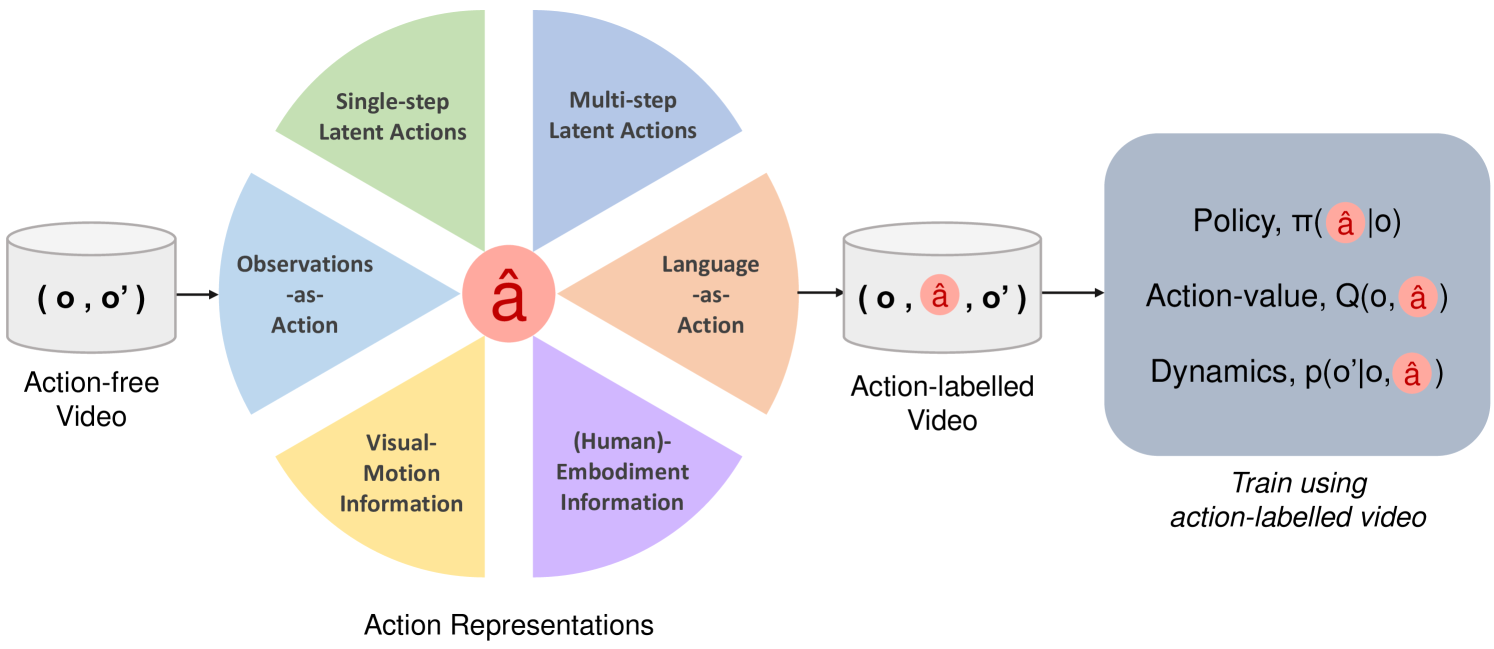
\includegraphics[width=1.0\linewidth]{./chapter5/media/RecoveringActionFepresentationsFromVideo_1}
	\caption[To label action-free videos, an Alternative action $\hat{a}$ can be derived from video data instead of the missing Action $a$]{To label action-free videos, an Alternative Action $\hat{a}$ can be derived from video data instead of the missing action $a$ \cite{McCarthy_2025}.}
	\label{fig:RecoveringActionFepresentationsFromVideo_1}
\end{figure}


The main challenges for transferring video-extracted knowledge to robotics are: 
\begin{enumerate}
    \item \textbf{Missing action labels}: Most video datasets do not contain explicit robot action annotations, which are required for learning robot control policies \cite{McCarthy_2025}.
    \item \textbf{Distribution shift}: There exists a significant domain gap between human/internet demonstrationvideos and robot execution. This includes differences in visual appearance, embodiment, dynamics, and behavior patterns, which can severely degrade the generalization of models trained on video data when applied to robotic tasks \cite{McCarthy_2025}.
\end{enumerate}

% ToDo: real world datasets with no robot labels
In many real-world video datasets, explicit robot action labels (e.g. joint velocities or torques) are not available.
% Problem. 
Raw video data provides only state transitions pairs $(o_t, o_{t+1})$, without access to the corresponding actions $a_t$. This makes it difficult to directly apply \ac{BC} or \ac{RL} methods, which typically require triplets of the form $(o_t, a_t, o_{t+1})$. Recovering such low-level actions directly from video is a challenging problem due to ambiguity and the lack of physical interaction information \cite{McCarthy_2025}. 
% Solution.
% To overcome this limitation, recent approaches introduce an Alternative Action Representation $\hat{a} \in \hat{A}$ within the alternative-action Space $\hat{A}$ so that transitions can be relabeled as $(o_t, \hat{a}_t, o_{t+1})$. 
To overcome this limitation, recent approaches introduce an \textbf{Alternative Action Representation} $\hat{a} \in \hat{A}$, which can be used to relabel action-free videos and enable video-to-robot transfer despite missing action labels and distribution shift, see Figure \ref{fig:RecoveringActionFepresentationsFromVideo_1}.

Formally, this induces a relabeling of video transitions as:
\begin{equation}
    (o_t, o_{t+1}) \;\rightarrow\; (o_t, \hat{a}_t, o_{t+1}), \quad \hat{a}_t \in \hat{A}.
\end{equation}

% To overcome this limitation, recent approaches introduce an Alternative Action Representation Space $\hat{A}$, where an alternative action $\hat{a} \in \hat{A}$ can be derived from video data, allowing transitions to be relabeled as $(o_t, \hat{a}_t, o_{t+1})$. 



% Video data provides state transition information in the form of $(o_t, o_{t+1})$ pairs, which can be used to derive alternative action representations $\hat{a}$ that capture the underlying behavior or intent of the observed transitions. By learning to predict $\hat{a}$ from video observations, the model can capture high-level behavioral patterns that are relevant for robotic control, even in the absence of direct action labels.

% To address these challenges, recent approaches introduce an alternative action representations $\hat{a} \in \hat{A}$ can be derived from video data, which can be used to label action-free videos and enable video-to-robot transfer despite missing action labels and distribution shift, see Figure \ref{fig:RecoveringActionFepresentationsFromVideo_1}. 

\subsection{What is an Alternative Action Representation?}
Formally, an alternative action representation is defined as
\begin{equation}
    \hat{a} \in \hat{A},
\end{equation}
where
$\hat{A}$ denotes an Alternative latent/abstract Action Representation Space. 
Instead of modeling actions as raw robot control signals, actions are encoded in a semantic feature space that captures high-level behavior such as grasping, moving, or pushing. In other words, $\hat{A}$ captures what actions \textit{mean}, rather than how it is executed at the motor level \cite{McCarthy_2025}.
% which are easier to infer from video, rather than the raw motor commands.
The key idea is that the action $\hat{a}$ serves as a proxy for the missing robot action labels $a$, allowing the model to learn from video data without requiring explicit action annotations. Later, $\hat{a}$ can be decoded or translated into the robot's actual action space if a mapping $f: A \to \hat{A}$ exist \cite{Wang2023MimicPlayLI, Wen2023AnypointTM, Du2023LearningUP}. Otherwise, they still provide valuable structure \cite{Bhateja2023RoboticOR, Schmidt2023LearningTA}. However it is also valid to define a $\hat{A}$ that requires labelled video (e.g., language captions) \cite{McCarthy_2025}.


\paragraph{Example} 
Consider a video of a human performing a pick-and-place task. The raw video data provides visual observations of the human's hand and the objects being manipulated, but does not include explicit robot action labels such as joint angles or end-effector velocities.
\begin{itemize}
    \item The \textbf{Video Encoder} extracts visual features (what is being done), see section~\ref{sec:VideoEncoder}.
    \item The \textbf{Action Embedding Space $\hat{A}$} captures \textit{abstract actions} such as \textit{reach}, \textit{grasp}, \textit{move up}.
    \item The \textbf{Policy $\pi_{alt}( \hat{a}_t | o_t, c), \quad \hat{a}_t \in \hat{A}$} predicts the next action \textit{in this latent action space} based on current visual observations and probably some additional context information $c$, see section~\ref{sec:AlternativeActionPolicy}.  
    \item Later, a \textbf{Decoder} $\pi(a_t \mid \hat{a}_t, o_t)$ or \textbf{Alignment Model $a_t = f_{align}(\hat{a}_t)$} maps these latent actions to the robot's real motor commands, see section~\ref{sec:AlternativeActionDecoder}.    
\end{itemize}



\paragraph{Why is $\hat{A}$ Useful?}

Working in the alternative action space $\hat{A}$ offers several advantages. 
\begin{itemize}
    \item \texttt{Bridging the Domain Gap:} $\hat{A}$ bridges the gap between human video data and robot control by focusing on action semantics rather than platform-specific motor commands \cite{McCarthy_2025}. 
    
    \item \texttt{Learning from Weak Labels:} $\hat{A}$ enables learning from raw or weakly labeled videos, since inferring high-level actions from video is easier than recovering low-level motor commands \cite{McCarthy_2025}.
    
    \item \texttt{Transferable Representations Across Embodiments:} $\hat{A}$ supports transfer across embodiments, because the same semantic action (e.g. ``open drawer'') can be instantiated by different robots with different kinematics \cite{McCarthy_2025}.
    % \item \texttt{Structured learning:} $\hat{A}$ provides a structured representation that can be used for learning policies, dynamics models, and value functions in a more data-efficient and generalizable way if $\hat{A}$ is well-structured, minimal, disentangled, and semantically consistent across embodiments.

    \item \texttt{Structured Learning:} A well-structured representation $\hat{A}$ that is minimal, disentangled, and semantically consistent across the state space encodes meaningful action information. This makes it easier to learn models that are predictive of both future observations (i.e. learning $p_{\text{alt}}(o_{t+1} \mid \hat{a}_t, o_t)$ instead of $p(o_{t+1} \mid o_t)$) and robot actions (i.e., learning $\pi(a_t \mid \hat{a}_t, o_t)$ instead of $\pi(a_t \mid o_t)$), leading to more data-efficient and generalizable policies, dynamics models, and value functions \cite{McCarthy_2025, Rybkin2018LearningWY, Bruce2024GenieGI}.
    The choice of abstraction level for $\hat{A}$ also plays a crucial role: 
    \begin{itemize}
        \item \textbf{Higher-level or longer-horizon representations} $\hat{A}$ (such as language-based actions) can benefit performance in complex, long-horizon tasks by providing broader context and intent. This is because they capture more abstract and semantically meaningful information that can guide decision-making over longer time scales, which is particularly beneficial for tasks that require planning and reasoning about future consequences \cite{McCarthy_2025}.
        \item \textbf{Lower-level or shorter-horizon representations} $\hat{A}$, which retain more fine-grained information, may be more effective for accurately reconstructing or decoding the original robot actions $a_t$ from the alternative actions $\hat{a}_t$ \cite{McCarthy_2025}.
    \end{itemize}
\end{itemize}
% It can improve data efficiency and generalization, since a well-structured alternative action space $\hat{A}$ that is minimal, disentangled, and semantically consistent allows both $\pi(\hat{a}_t \mid o_t)$ and $\pi(a_t \mid \hat{a}_t, o_t)$ to be learned more easily and with fewer samples.
% The desired characteristics are:


Once $\hat{A}$ is defined, the same representation can be used for example for:
\begin{itemize}
    \item policies $\pi_{\hat{A}}(\hat{a}_t \mid o_t)$ \cite{Schmidt2023LearningTA},
    \item dynamics models $p_{\hat{A}}(o_{t+1} \mid o_t, \hat{a}_t)$ \cite{Bruce2024GenieGI} or
    \item state-action value functions $Q_{\hat{A}}(o_t, \hat{a}_t)$ \cite{Bhateja2023RoboticOR},
\end{itemize}
which further encourages consistent and transferable action abstractions.


% Once $\hat{A}$ is defined, the same representation can be used not only for policies $\pi_{\hat{A}}(\hat{a}_t \mid o_t)$, but also for dynamics models $p(o_{t+1} \mid o_t, \hat{a}_t)$ or value functions $Q(o_t, \hat{a}_t)$, which further encourages consistent and transferable action abstractions.


%---------
% By learning to predict $\hat{a}$ from video observations, the model can capture high-level behavioral patterns that are relevant for robotic control, even in the absence of direct action labels.


% Action free Video data often lacks on explicit action labels for robotics. But it is difficult to recover these missing robot action labels from video data directly. 

% The Idea is to label the videos with an alternative Action $\hat{a} \in \hat{A}$ from an Alternative Representation Space $\hat{A}$, which should be easier than directly derive the specific robot action labels from video data.

% representations $\hat{a}$ from video data, which can serve as proxies for the missing action labels. 


% from $(o_t, o_{t+1})$ to $(o_t, \hat{a}_t, o_{t+1})$.

% To address this, we can derive alternative action representations $\hat{a}$ from video data, which serve as proxies for the missing action labels. These alternative representations can be obtained through various methods, such as:


% Goal: Recovering the missing action representations from video

\subsection{Categories of Alternative Action Representations}
\label{sec:CategoriesOfAlternativeActionRepresentations}


\begin{figure}[h]
	\centering
	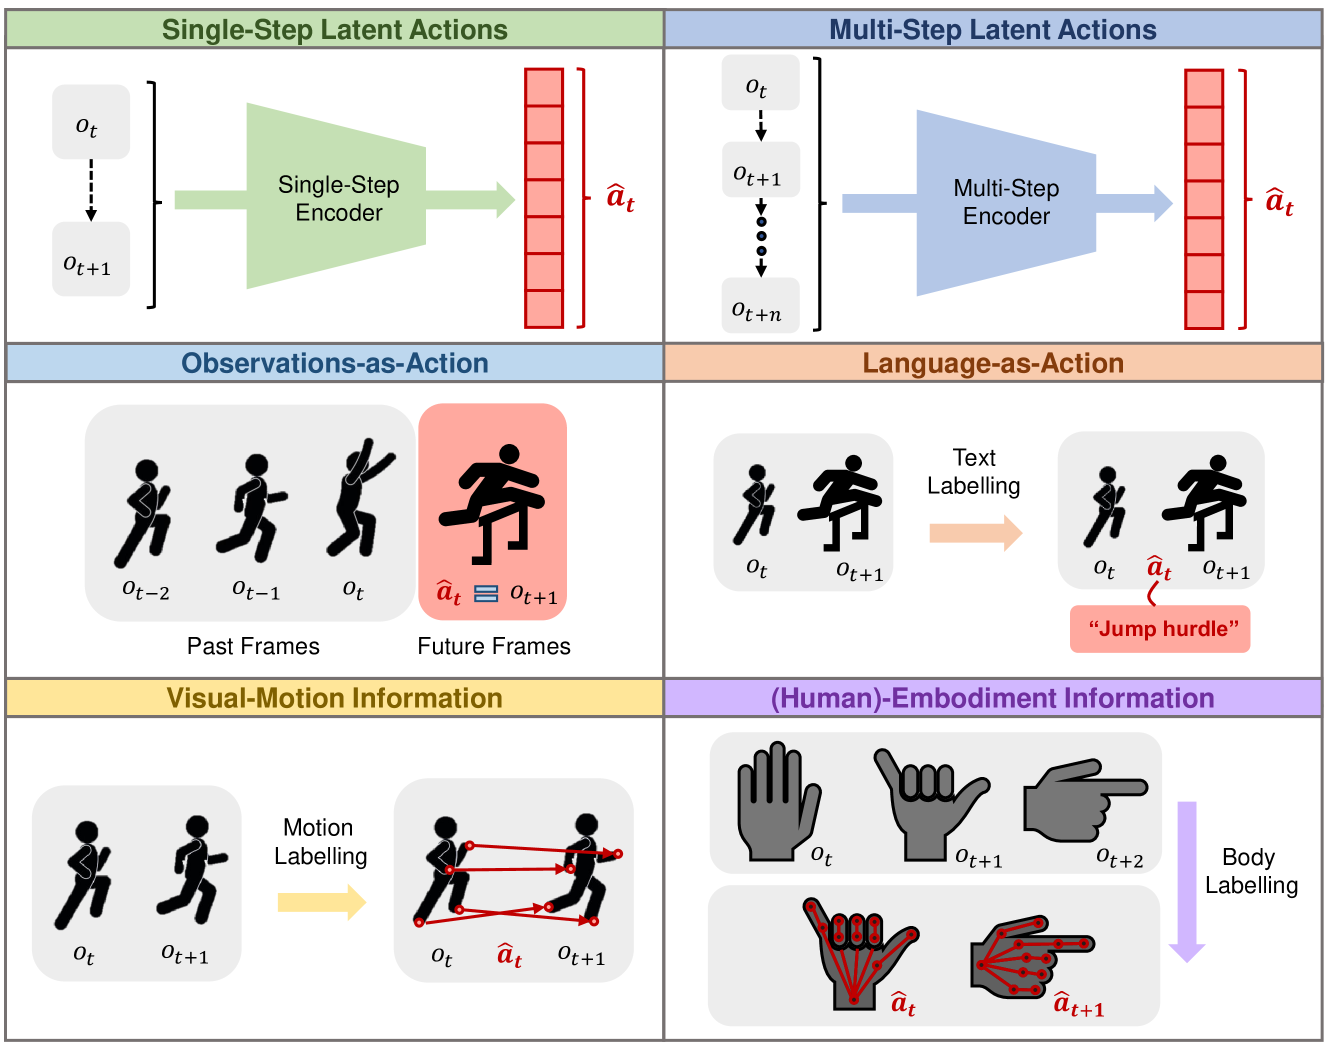
\includegraphics[width=1.0\linewidth]{./chapter5/media/RecoveringActionFepresentationsFromVideo_2}
	\caption[Categories of Alternative Action Representations that can be learned or obtained from video data.]{Categories of Alternative Action Representations that can be learned or obtained from video data
 \cite{McCarthy_2025}.}
	\label{fig:RecoveringActionFepresentationsFromVideo_2}
\end{figure}


Their exist different approaches to derive alternative action representations $\hat{a} \in \hat{A}$ from video data. These methods differ in how actions are represented and which information is extracted from visual observations \cite{McCarthy_2025}.







\paragraph{Single-step Latent Actions:}

These approaches learn latent actions in vectorized forms (=embedding) that describe the transition from one observation to the next \cite{McCarthy_2025}:
\begin{equation}
\hat{a}_t : o_t \rightarrow o_{t+1}
\end{equation}

\paragraph{Methods:}
The latent action $\hat{a}_t$ can be learned for example through:
\begin{itemize}
    \item \textbf{\ac{FDM}} $p(o_{t+1} \mid \hat{a}_t, o_t)$, which predict future observations from the current observation and latent actions \cite{Bruce2024GenieGI, Edwards2018ImitatingLP, Schmidt2023LearningTA, Ye2024LatentAP, Rybkin2018LearningWY}.
    \item \textbf{\ac{IDM}} $p^{-1}(\hat{a}_t \mid o_t, o_{t+1})$, which infer the latent action responsible for a transition \cite{Schmidt2023LearningTA, Bruce2024GenieGI}. 
    % To hinder the IDM from copying the entire observation $o_{t+1}$ into the latent action $\hat{a}_t$, the model is trained with some form of regularisation, such as a quantization bottleneck \cite{McCarthy_2025, Schmidt2023LearningTA, Bruce2024GenieGI}.
\end{itemize}

\paragraph{Limitations:}
\begin{itemize}
    \item Often capture all visual changes, not only agent actions \cite{McCarthy_2025}.
    \item May omit important non-visual information such as forces or contact dynamics \cite{McCarthy_2025}.
\end{itemize}








\paragraph{Multi-step Latent Actions:}

These methods encode behaviors across multiple time-steps in a single embedding:
\begin{equation}
\hat{a}_t : o_t \rightarrow o_{t+k}
\end{equation}

Instead of modeling individual actions, they capture higher-level behavioral patterns or latent plans \cite{McCarthy_2025}.
The key idea is to learn a compact latent representation of a \emph{skill} or \emph{sub-policy} that summarizes an entire sequence of actions. These representations are more abstract, goal orientated and can encode longer-horizon information, which may be beneficial for complex tasks \cite{RoseteBeas2022LatentPF, Cui2022FromPT, lynch2020learning}. 

For example these ``skill embeddings'' can capture structures such as ``reach the object'', ``move the arm to the target location'', or ``grasp and lift'', which can later be decoded into a full action sequence.


% Instead of modeling individual actions, they capture higher-level behavioral patterns or latent plans. These representations are more abstract, goal orientated and can encode longer-horizon information, which may be beneficial for complex tasks. 

% The key idea is that the model does not explicitly output every intermediate action, but instead learns a compact representation of a \emph{skill} or \emph{sub-policy} that executes a sequence of actions over time. These representations are more abstract, goal orientated and can encode longer-horizon information, which may be beneficial for complex tasks. 

% In this way, the representation captures higher-level structure such as ``reach the object'', ``move the arm to the target location'', or ``grasp and lift'', which can then be decoded into a full action sequence. This encourages the model to compress long action trajectories into a compact latent ``skill embedding'' that captures the essence of the behavior, rather than modeling every low-level action step.



\paragraph{Methods:}
\begin{itemize}
    \item \textbf{Variational Sequence Models:} These methods use \acp{VAE} to encode motion trajectories or sequences of observations into a latent variable $z$ that captures the underlying behavior. The VAE is trained to reconstruct the original trajectory from the latent representation \cite{Wang2023MimicPlayLI}.    
    % Variational auto-encoding of motion or trajectory representations 
    \item \textbf{Video-Language Contrastive Learning:} Aligns video segments with natural language descriptions of behaviors \cite{fan2022minedojo, Lifshitz2023STEVE1AG, Sontakke2023RoboCLIPOD}.
    \item \textbf{Supervised Contrastive Learning:} Pulls on a action-labeled dataset, videos with the same or similar action labels together in latent space, while pushing videos with different action labels apart \cite{ChaneSane2023LearningVP, Chen2021LearningGR}.
    \item \textbf{Self-Supervised Clustering Approaches:} Group similar motion patterns or trajectories into clusters without requiring labels, with each cluster representing a reusable skill or behavior primitive \cite{Xu2023XSkillCE}.
    \item \textbf{Further Approaches:} Presented in the works of Tomar et al. \cite{tomar2023video}, Pertsch et al. \cite{Pertsch2022CrossDomainTV}, and Cai et al. \cite{Cai2023GROOTLT}. 
    % include hierarchical sequence models and latent plan representations (e.g., Pertsch et al., Cai et al.), which explicitly model skills as temporally extended latent variables.
\end{itemize}

\paragraph{Limitations:}
\begin{itemize}
    % Quellen sollten passen
    \item Often produce abstract and long-horizon representations that may lose fine-grained control details and be harder to align with low-level robot actions \cite{kim2026hierarchical, liang2025clam}.
\end{itemize}






\paragraph{Observations-as-Actions:}

These approaches directly use (encoded) future observations as action representations:
\begin{equation}
    \hat{a}_t = o_{t+k}.
\end{equation}
Future observations provide information about the intended behavior or goal state \cite{McCarthy_2025}.

\paragraph{Methods:}
\begin{itemize}
    \item \textbf{Next-Observation-as-Action:} Uses the next observation $o_{t+1}$ as the $\hat{a}_t$ label and provides information regarding the action that should be taken \cite{Du2023LearningUP, Thomas2023PLEXMT, he2024large}.
    \item \textbf{Observations-as-Subgoals:} Uses future observations as intermediate goals to guide action selection \cite{Black2023ZeroShotRM, park2023hiql, Bhateja2023RoboticOR}. There exist different options to select the future observation that during training stage: 
    \begin{itemize}
        \item \textbf{Fixed Time Horizon:} Uses observations that are fixed $k$ time steps in advance \cite{Black2023ZeroShotRM, Du2023LearningUP}.
        \item \textbf{Random Time Horizon:} Uses observations that are a randomly sampled number of time steps in advance \cite{Bhateja2023RoboticOR}.
        \item \textbf{Key-Frame Selection:} Identifies critical states in a trajectory that can serve as action representations \cite{Pertsch2019KeyframingTF, liu2023learning}, see table \ref{tab:keyframes_pickplace}.
        
        \begin{table}[h]
            \centering
            \begin{tabular}{|c|l|l|}
                \hline
                \textbf{Time Step} & \textbf{Frame Description} & \textbf{Significance} \\
                \hline
                $t_0$ & Arm over table & Start \\
                $t_1$ & Arm approaches cup & Intermediate state \\
                $t_2$ & \textbf{Hand touches cup} & \checkmark\ Key-frame \\
                $t_3$ & Cup is lifted & Intermediate state \\
                $t_4$ & \textbf{Cup over target} & \checkmark\ Key-frame \\
                $t_5$ & Cup is placed & End \\
                \hline
            \end{tabular}
            \caption{Example Key-Frames in a Pick-and-Place Sequence}
            \label{tab:keyframes_pickplace}
        \end{table}
    \end{itemize}
\end{itemize}

\paragraph{Limitations:}
\begin{itemize}
    \item Future observations may not uniquely determine the underlying action \cite{A_hierarchical_representation_for_future_action_prediction}.
    \item High-dimensional visual observations can increase learning complexity \cite{A_hierarchical_representation_for_future_action_prediction, Losey2021LearningLA}.
\end{itemize}






% ToDo: Quelle 306, 7 evtl. hinzufügen
\paragraph{Language-as-Actions:}

Natural language descriptions can be used as high-level action representations for example by captioning video frames with language instructions that describe the observed behavior \cite{belkhale2024rt, shi2024yell, xiang2024pandora}:
\begin{equation}
\hat{a}_t = \texttt{"pick up the cube"}.
\end{equation}
Language-based actions provide semantic supervision and enable integration with \acp{LLM} \cite{Du2023VideoLP}, which can facilitate more complex reasoning and planning.

\paragraph{Methods:}
\begin{itemize}
    % ToDo: Quellen für diese beide Stichpunkte
    \item Video-to-Text Models \cite{McCarthy_2025}
    \item \acp{VLM} and variants of them \cite{McCarthy_2025}
\end{itemize}

\paragraph{Methods for Missing Language Captions:}
Video datasets may not always contain usable language captions. To address this, several methods can be used to generate or enhance captions for video data: 
\begin{itemize}
    % ToDo: Hier evtl. nochmal die Quellen nachprüfen
    % \item Language-captioned video datasets \cite{Grauman2021Ego4DAT}
    \item Process and enhance standard captions to generate more detailed action descriptions, for example by using \acp{LLM} or \acp{VLM} \cite{Mu2023EmbodiedGPTVP}.
    \item Usage of automated or semi-automated video captioning methods \cite{Mu2023EmbodiedGPTVP}
\end{itemize}


% ToDo: Quellen überprüfen und evtl. bessere suchen
\paragraph{Limitations:}
\begin{itemize}
    \item Language is often coarse and omits low-level control details \cite{McCarthy_2025}.
    \item Requires annotated or captioned video data \cite{McCarthy_2025}.
\end{itemize}






\paragraph{Visual Motion Information:}

These approaches define actions using visual motion cues extracted from video sequences \cite{McCarthy_2025}. The underlying assumption is that temporal changes in visual observations (motion patterns) contain implicit information about the actions responsible for observed state transitions. For example, the direction, magnitude, and trajectory of movement can provide information about the intended behavior, goal, or interaction dynamics \cite{yanokura2020understanding, Tokmakov17}.

\paragraph{Methods:}
\begin{itemize}
    \item \textbf{2D or 3D Point Trajectories:} Tracking objects or hands \cite{Wen2023AnypointTM, Yuan2024GeneralFA} via off-the-shelf point trackers \cite{karaev2024cotracker}
    \item \textbf{Optical Flow Predictions:} Capturing  how image regions move between consecutive video frames \cite{Ko2023LearningTA, xu2022gmflow}
    % \item Optical flow prediction, which captures how image regions move between consecutive video frames
    \item \textbf{Visual Action Arrows:} Representing movement direction and magnitude directly in the image \cite{Nasiriany2024PIVOTIV}
    \item \textbf{Structure-from-Motion Approaches:} Reconstructing 3D scene geometry and camera motion from video in order to recover information about underlying physical interactions \cite{Wang2023ManipulateBS, Yuan2021DMotionRV, Yang2023LearningIR}
\end{itemize}

\paragraph{Limitations:}
\begin{itemize}
    \item Motion estimates can be noisy or ambiguous \cite{booij2010efficient}.
    \item Visual motion does not always correspond directly to robot actions \cite{booij2010efficient}.
\end{itemize}




% ToDo: Quellen neu anordnen + überprüfen wo welche gebraucht wird.
% ToDo: Quelle 203 evtl. hinzufügen
\paragraph{(Human)-Embodiment Information:}

These approaches explicitly model human body structure and kinematics \cite{McCarthy_2025, Bharadhwaj2023TowardsGZ, Shaw2022VideoDexLD, Bahl2023AffordancesFH, Qin2022FromOH, Qin2021DexMVIL}. 
In contrast to generic motion-based methods, which focus on pixel or object movement, these approaches aim to represent the \emph{agent performing the action} using structured human pose information. 
Embodiment-specific information such as hand poses, affordances, or trajectories can provide useful cues about the intended actions and interactions in the video, which can be transferred to robotic embodiments \cite{rong2020frankmocap, Shan2020UnderstandingHH}.
For example, an alternative action representation can be defined as:
\begin{equation}
    \hat{a}_t = \text{hand pose at next time-step } t+1,
\end{equation}
which encodes the intended end-effector movement and can be associated with actions such as reaching, grasping, or manipulating objects. Animal embodiment data could also be useful \cite{peng2020learning}.
% which can be used to infer actions such as reaching, grasping, or manipulating objects.

\paragraph{Methods:}
\begin{itemize}
    \item \textbf{Human Pose Estimation:} Estimating full-body kinematics \cite{Bharadhwaj2023TowardsGZ}.
    \item \textbf{Hand Pose Estimation and Trajectory Tracking:} Estimating hand pose and tracking hand trajectories \cite{rong2020frankmocap, Shan2020UnderstandingHH}.
    \item \textbf{Affordance Prediction:} Predicting for example graspable regions, interaction points, and grasp trajectories \cite{Bahl2023AffordancesFH, Bharadhwaj2023TowardsGZ}.
    \item \textbf{Object- and Hand-Mask Conditioned Representations:} Focusing on regions of the video relevant for action understanding while ignoring irrelevant background information\cite{Bharadhwaj2023TowardsGZ}.
\end{itemize}

\paragraph{Limitations:}
\begin{itemize}
    \item Human embodiment is structurally different from robotic embodiments, limiting direct transferability.
    \item Accurate pose and hand tracking or estimation can be unreliable in cluttered or occluded scenes.
    \item Focuses on human-centric actions, which may not generalize to non-human interaction styles.
\end{itemize}




\paragraph{Inverse Dynamics Model (IDM) for Pseudo-Action Labels:}
It's not an alternative action representation in the strict sense, but it is a method to recover missing action labels from video data.
These methods train an inverse dynamics model on robot data and use it to infer pseudo-action labels for action-free (human) videos \cite{Baker2022VideoP, Torabi2018BehavioralCF, Schmeckpeper2020ReinforcementLW}, which can then be used for learning policies \cite{McCarthy_2025}:
\begin{equation}
p^{-1}(a_t \mid o_t, o_{t+1}).
\end{equation}

\paragraph{Limitations:}
\begin{itemize}
    \item Require action-labeled robot data for model training \cite{Baker2022VideoP, Torabi2018BehavioralCF, Schmeckpeper2020ReinforcementLW}.
    \item Domain shift between demonstration videos and robot execution \cite{Baker2022VideoP, Schmeckpeper2020ReinforcementLW, Kim2023GivingRA}.
\end{itemize}







  \chapter{Robot Learning Fundamentals}


\section{Robot Learning - Learning Objectives}


\section{Robot Learning - Approaches}


\section{Vision Language Action Models}
  \chapter{Challenges and Future Directions}

Despite significant progress in imitation learning and video-based robotic learning, several fundamental challenges still limit the deployment of robust and generalizable robotic systems. Current methods often struggle with data availability, computational scalability, domain transfer, and efficient policy learning. At the same time, emerging architectures such as diffusion models, world models, and causally-aware systems provide promising directions for future research.


\section{Data}

% Problem: Data Availability
The performance of modern Robotic models strongly depends on the availability, diversity, and quality of demonstration data. However, collecting large-scale robotic datasets remains expensive and time-consuming, particularly when expert annotations or robot demonstrations are required. Existing datasets are often domain-specific, weakly balanced, or limited to narrow task distributions, reducing the ability of models to generalize to unseen environments, objects, or robot embodiments.

% Solution: Internet videos
One promising approach is the use of internet videos, which provide a vast amount of diverse visual demonstrations at a significantly lower collection cost than robot-specific datasets. However, such data often lacks precise action annotations and task labels.

% Solution: Weak supervision and self-supervised learning
To address this limitation, weakly supervised learning methods utilize coarse or incomplete labels, such as video captions, task descriptions, or automatically generated annotations, instead of relying on expensive frame-by-frame expert labeling. Similarly, self-supervised learning objectives enable models to learn useful visual and temporal representations directly from raw video data. Common objectives include predicting future video frames, reconstructing masked observations, or learning representations that remain consistent across temporally related frames. These approaches allow robots to exploit large amounts of unlabeled data while reducing the dependence on manual annotation.

% Solution: Active Learning
Another challenge is the efficient acquisition of high-quality labels. Active learning addresses this issue by allowing a model to strategically select the most informative or uncertain samples for annotation rather than labeling entire datasets uniformly. For example, a robot may request human annotations only for demonstrations in which its predictions are uncertain, thereby reducing annotation costs while maximizing the benefit of labeled data.

% Solution: Active physical interaction
Beyond passive observation, future imitation learning systems may also integrate active physical trials, where robots interact directly with their environment to refine policies learned from demonstrations. Such interaction-based learning combines the strengths of imitation learning and reinforcement learning, enabling robots to adapt to environmental variations, recover from failures, and acquire knowledge that is difficult to infer from observation alone.




% Problem: data efficiency
Another important challenge is sample efficiency. Many high-capacity imitation learning and RL methods still require large amounts of demonstrations or interaction data. Current approaches therefore investigate meta-learning, contrastive representation learning, and one-shot or few-shot imitation learning to reduce data requirements. Goal-conditioned RL and Representation Learning have also shown improved data efficiency, although robust learning from weakly-labeled or noisy demonstrations remains an open problem.


% Solution: data efficiency and availability
Future research must focus not only on improving generalization, but also on enabling rapid adaptation to new tasks, robots, and environments. Achieving this level of adaptability is considered a key requirement for scalable and general-purpose robotic intelligence.



% Data Availability and Annotation
% - To overcome the data sparsity, use internet videos and weak supervision, self-supervised objectives 

% Improving Data Annotation 
% - Active Learning: Strategically select informative video data for labeling
% - Integrate active physical trials (robot interaction) in Imitation Learning

% Sample Efficiency
% - Approaches: meta-learning, contrastive objectives, and one/few-shot imitation
% - Data-efficient approaches: feature extraction, goal-conditioned RL, some hybrid models --> currently problems with weakly-labeled data

% Tackling data efficiency and availability
% - Goal: Enhance generalization and quick adaptation to new tasks/environments.
% - Key Requirement: New methods must ensure quick adaptation to new tasks, robots & environments, moving beyond simple generalization




\section{Computional Costs}
% Problem:
The increasing adoption of large-scale transformer architectures and multimodal foundation models has significantly improved robotic perception and policy learning. However, these advances come at the cost of high computational and memory requirements.

State-of-the-art Vision-Language-Action models often require substantial GPU resources during both training and inference. This creates major deployment challenges for real-world robotic systems, especially on embedded or resource-constrained platforms where real-time execution is required.

% Solution:
% ToDo: Quelle für potential directions
Future work must therefore address efficient scaling strategies for both data and model architectures. Potential directions include for example lightweight transformer designs, modular architectures and model compression techniques.

% High computational costs of SOTA multi-modal and large-scale transformer architectures --> real-time execution <-> Robot hardware

\section{Domain Shift}
% Problem
A persistent challenge in imitation learning is the domain shift between
human demonstrations and robot execution. In particular, transferring skills from humans to robots is difficult because of differences in appearance, motion dynamics of task execution, embodiment, environment and action spaces. 
% This problem is commonly referred to as the embodiment gap.

% Solution
Current approaches attempt to learn domain-invariant or domain-adaptive representations using hybrid and multi-modal architectures, image translation techniques, or context-aware feature learning. Methods such as adversarial learning, keypoint-based transfer, and CycleGAN-based translation can partially reduce visual discrepancies between domains. However, translation artifacts, inaccurate pose estimation, and misaligned action representations still limit robust skill transfer.

% Future Directions
Future research will likely focus on more robust sim-to-real transfer methods, continual learning strategies during inference, and advanced domain adaptation techniques. Multi-modal learning approaches that integrate additional sensory modalities, such as force or tactile feedback, may further reduce the dependence on purely visual transfer. In addition, causal reasoning and few-shot adaptation methods could improve the transfer of manipulation skills across different robots and environments. Furthermore, researchers should investigate in attention mechanisms, unsupervised techniques, and transformer-based architectures.
% , which may also help to mitigate the domain shift problem.


% Domain Shift and Embodiment Gap

% Translation artifacts, misaligned action representations, imperfect pose estimation
% --> Approaches: adversarial learning, keypoint-based transfer, CycleGANs

% Need of domain-invariant or domain-adaptive features
% --> Approaches: hybrid- & multi-modal models, image/context translation 


% Tackling domain shift
% Future Directions: 
% - adversarial training, meta-learning Multi-modal strategies, Sim-to-real transfer strategies, continual learning
% - Causal reasoning and few-shot learning for skill transfer
% - Investigating in attention mechanisms, unsupervised techniques, and transformer-based architectures


\section{Emerging techniques and architectures}

\subsection{Diffusion models}
\subsection{World models}
\subsection{Integration of causal reasoning}

\section{Evaluation Metrics and Benchmarks}
Another major challenge is the lack of standardized evaluation metrics and benchmarking protocols for imitation learning and video-based robot learning. Current evaluations are often task-specific and rely on custom experimental setups, making fair comparisons between methods difficult.

Existing benchmarks primarily focus on task success rates, while aspects such as robustness, generalization, sim-to-real transfer, and adaptability are often insufficiently evaluated. Moreover, the design of a benchmark strongly influences research directions by implicitly prioritizing certain capabilities over others. Table \ref{tab:benchmark} summarizes a three prominent benchmarks and their principal focus.


% \textbf{Short notes on the three benchmarks.} 
% CALVIN become a de-facto standard for evaluating long-horizon, language-conditioned policy learning and compositional reasoning, by providing large-scale, compositional interaction data with tasks that require planning and instruction grounding. RLBench is a prominent benchmark for evaluating few-shot and multi-task manipulation, enabling consistent comparisons of meta-learning and generalization techniques. RoboTube focuses on learning from human demonstrations and on human-to-robot transfer, emphasizing sim-to-real metrics and the use of large, video-derived demonstration corpora.
% Table \ref{tab:benchmark} summarizes a three prominent benchmarks and their principal focus.

\begin{table}[htbp]
	\centering
	\small
	\begin{tabular}{|p{2.2cm}|p{6.0cm}|c|p{4.4cm}|}
		\hline
		\textbf{Benchmark} & \textbf{Focus} & \textbf{\# of Tasks} & \textbf{Key metrics} \\
		\hline
		CALVIN & Long-horizon, language-conditioned, compositional tasks & 34 & Long-horizon multi-task language-conditioned control success \\
		\hline
		RLBench & Few-shot, meta- and multi-task learning; broad skill acquisition & 100 & Few-shot task success \\
		\hline
		RoboTube & Learning from human demonstrations; human-to-robot transfer & 50 & Policy success rate in RT-sim; sim-to-real transfer success \\
		\hline
	\end{tabular}
    \caption{Prominent benchmarks and their focus}
	\label{tab:benchmark}
\end{table}

% An important limitation of current benchmarks is the absence of explicit evaluation of causal understanding, whether a model truly understands physical interactions or merely exploits statistical shortcuts.
\textbf{The causal gap.} An important limitation of current benchmarks is that they primarily reward correlational, task-level success. They do not explicitly test whether an agent has learned causal relationships that govern object interactions and task dynamics. As a result, an agent may reach high success rates by exploiting statistical regularities in the training data rather than by acquiring a robust causal model. For example, a policy might learn that pushing a particular red button is followed by a light turning on, without understanding the causal mechanism. If the button's function were altered, an object's physical properties were changed, or an unobserved confounding factor were introduced, a correlational policy will often fail. 
% If the wiring is changed, or the object's mass or friction is altered, such a correlational policy will often fail.

\textbf{Towards causal evaluation protocols.} To close the causal gap \cite{?} propose evaluation protocols inspired by the Minimal Video Pairs (MVP) idea [207], adapted to robotic control. MVP forces models to distinguish minimally different scenarios by changing a single causal detail. 
% Applied to robotics, this suggests an "interventional" evaluation that perturbs the causal structure of the environment at test time. 
A potential protocol would proceed in two stages:
\begin{enumerate}
    \item Train agents using the standard benchmark dataset and metrics (as today).
    \item Evaluate robustness and causal understanding on a suite of interventional test tasks where underlying causal factors are systematically perturbed. Examples include changing object mass or friction, rewiring the causal relation between a switch and an effect, or introducing previously absent confounders (e.g., making a drawer stick).
\end{enumerate}

Under this protocol a purely correlational policy that overfits the training statistics is expected to fail on the perturbed tasks, while a model that internalizes causal relationships should either adapt its policy to the new dynamics or detect the distributional shift and trigger safer, more informed failure recovery strategies. Quantitatively, such a benchmark would report both standard task success and robustness metrics, such as performance drop under interventions, adaptation speed, and diagnostic measures of causal inference.

Developing and releasing such interventional benchmarks will provide a concrete, quantitative way to measure the benefits of causal reasoning in robotic manipulation, and will help steer the field toward methods that generalize in meaningful, physically grounded ways.


% Table \ref{tab:benchmark} shows the most prominent Benchmarks in a short overview overview and where their focus.

% \begin{table}[htbp]
% 	\centering
% 	\caption{Prominent benchmarks and their focus}
% 	\label{tab:benchmark}
% 	\small
% 	\begin{tabular}{|p{3.0cm}|p{6.0cm}|c|p{5.0cm}|}
% 		\hline
% 		\textbf{Benchmark} & \textbf{Focus} & \textbf{\# of Tasks} & \textbf{Key metrics} \\
% 		\hline\hline
% 		Calvin & Long-horizon, language-conditioned, compositional tasks & 34 & Long-horizon multi-task language-conditioned control success \\
% 		\hline
% 		RLBench & few-shot, meta- and multi-task learning; broad skill acquisition & 100 & Few-shot task success \\
% 		\hline
% 		RoboTube & Learning from human demonstrations; human-to-robot transfer & 50 & Policy success rate in RT-sim; sim-to-real transfer success \\
% 		\hline
% 	\end{tabular}
% \end{table}






% Evaluation Metrics and Benchmarks
% No standardized evaluatioin metrics/benchmarks for video-based robot learning
% Need of metrics that capture not only task success but also generalization, robustness and sim-to-real performance

% The design of a benchmark implicitly steers research priorities
% Causal Gap: None of the current benchmarks explicitly test causal understanding
% Need of a "Causal-CALVIN" or "Interventional RLBench" where the underlying causal structure (e.g., object physics) is perturbed to test for robustness against spurious correlations

  \chapter{Discover Selected Approaches}
In this chapter, we will explore some Imitation Learning approaches, that were applied to real robots to get a better practical understanding of the theoretical field. 

% ToDo: End-to-End trained
\section{Paper - Vid2Robot: End-to-end Video-conditioned Policy Learning with Cross-Attention Transformers}

Vid2Robot, a end-to-end video-based learning framework for robots. Given a human or robot video demonstration of a manipulation task and the robot's current visual observations, Vid2Robot directly produces corresponding robot actions in it's own environment. The Demonstration Video can be taken in a different environment or from a different viewpoint. Additionally, Vid2Robot exhibits emergent capabilities, such as successfully transferring observed motions from one object to another (see Figure~\ref{fig:Vid2RobotGeneralization}), and long-horizon composition, thus showcasing its potential for real-world applications.

\begin{figure}[!ht]
	\centering
	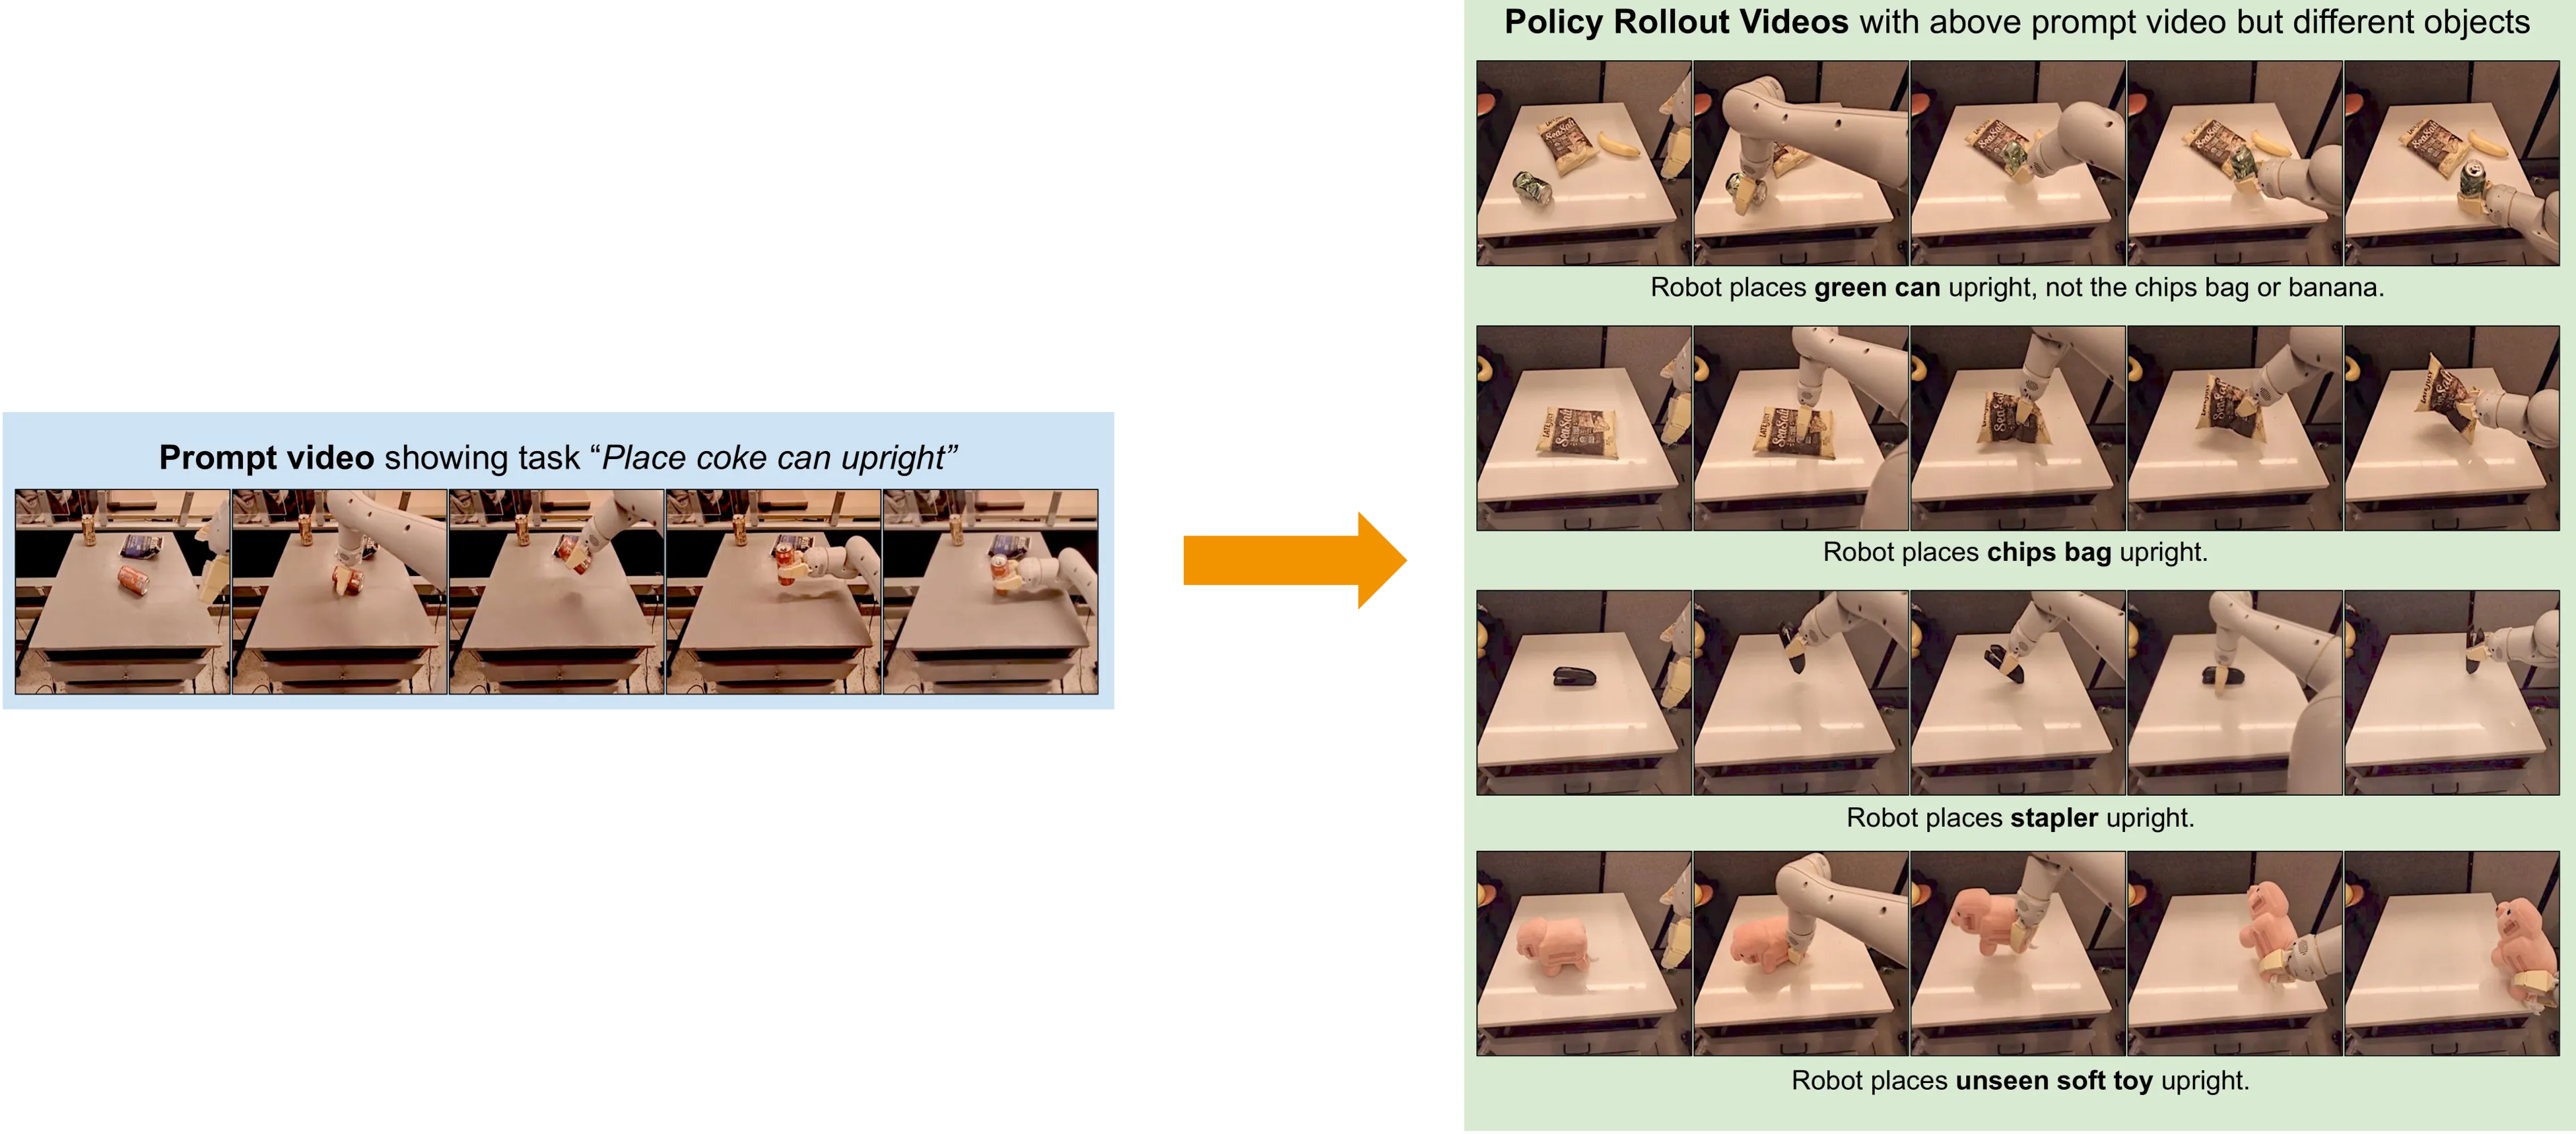
\includegraphics[width=1.0\linewidth]{./chapter8/media/Vid2Robot_Generalization.png}
	\caption[Vid2Robot can transfer observed motions from one object to another]{Vid2Robot can transfer observed motions from one object to another. \cite{?}.}
	\label{fig:Vid2RobotGeneralization}
\end{figure}



\subsection{Architecture}
\begin{figure}[!ht]
	\centering
	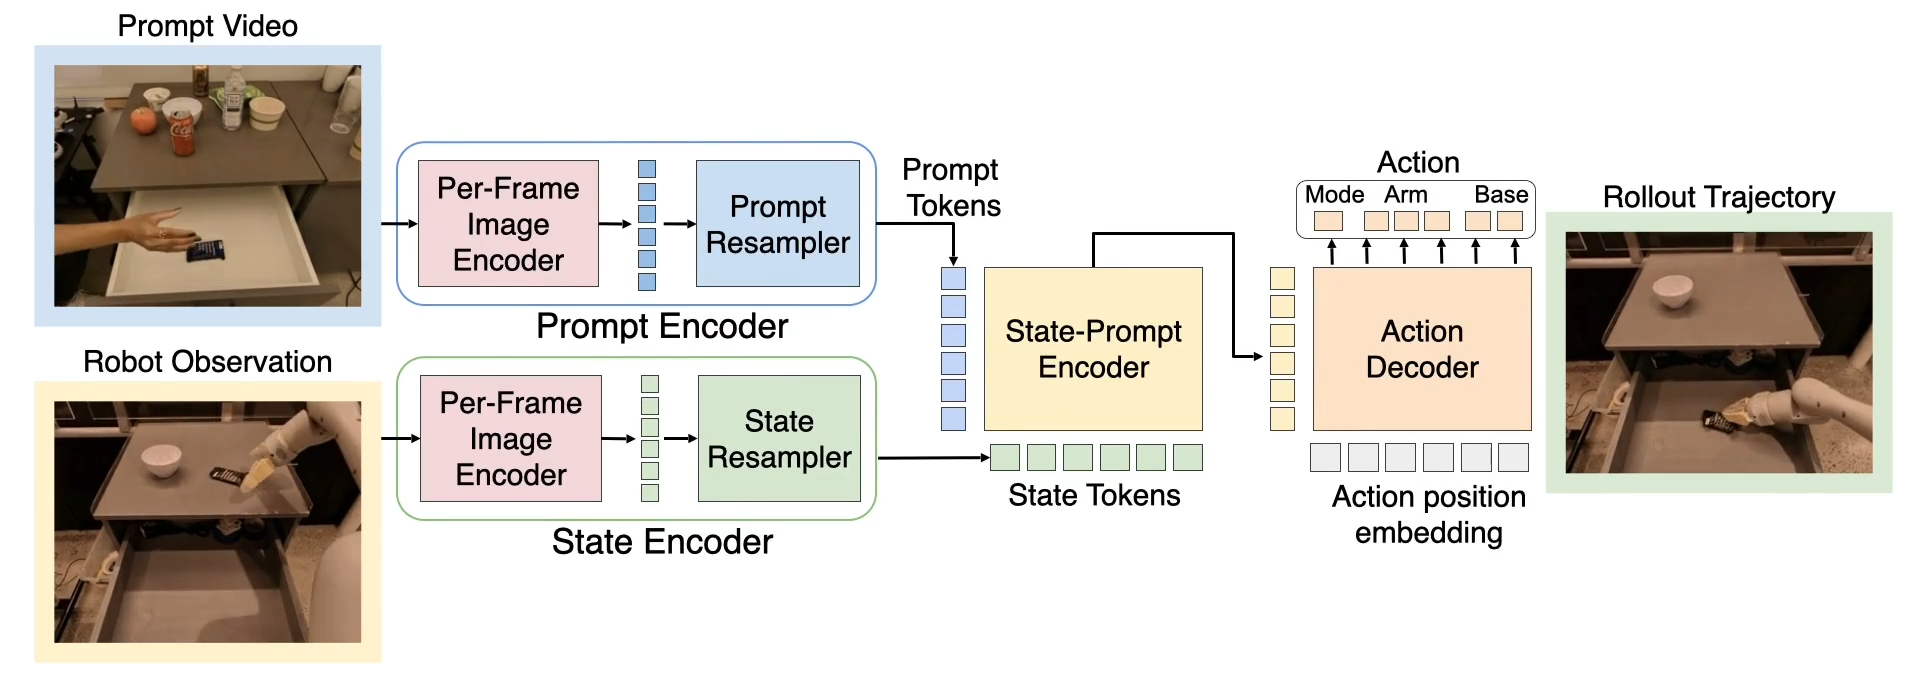
\includegraphics[width=1.0\linewidth]{./chapter8/media/Vid2Robot_Architecture.png}
	\caption[Vid2Robot Architecture]{Vid2Robot Architecture \cite{?}.}
	\label{fig:Vid2RobotArchitecture}
\end{figure}


% The core of Vid2Robot is a cross-attention transformer architecture that effectively fuses information from both the video demonstration and the robot's current observations, enabling it to learn complex manipulation tasks from human or robot demonstrations. 
The policy takes as input the prompt video and the current robot state and outputs robot actions. Vid2Robot consists of four
modules: 
\begin{enumerate}
    \item \textbf{Video Prompt Encoder}
        \begin{itemize}
            \item \textbf{Task:} 
            Encode demonstration video into meaningful representations that capture the essential information about the task being demonstrated.
            \item \textbf{Input:} A human or robot demonstration video of a manipulation task, which should be performed by the robot. 
            \item \textbf{Processing:} 
            Each frame of the demonstration video is first passed through a \texttt{Per-Frame Image Encoder}, which is implemented as a Vision Transformer and capture spatial visual information in each frame. Afterwards, a \texttt{Perceiver Prompt Resampler} aggregates frame tokens over time, reducing the number of tokens while preserving and restructuring temporal information, enabling temporal learning across frames. 
            % \item \textbf{Output:} A set of N tokens of dimension d, which form a compact semantic representation of the demonstration video that can be effectively used to condition the policy.
            \item \textbf{Output:} 
            The Prompt Video Encoder produces a set of d-dimensional \texttt{Prompt Tokens}, which form a compact semantic representation of the demonstration video, capturing \textit{what} needs to be done in the task and \textit{how} to do it. 
            \item \textbf{Purpose:} 
            Represent the demonstrated task goal and motion patterns.
        \end{itemize}
    \item \textbf{Robot State Encoder}
        \begin{itemize}
            \item \textbf{Task:} 
            Encode the robot's current visual observation about objects and the environment into meaningful representations.
            \item \textbf{Input:} The robot's observation, which includes the current and last k robot camera frames.
            \item \textbf{Processing:} 
            The Processing pipeline is the same as in the Prompt Video Encoder, where each frame is first passed through a \texttt{Per-Frame Image Encoder} and then aggregated over time using a \texttt{Perceiver State Resampler}. The weights of the \texttt{Per-Frame Image Encoder} between the Prompt Encoder and State Encoder are shared.
            % , which encourages the model to learn a shared visual representation space for both human and robot videos, thus facilitating better generalization and transfer of learned skills from human demonstrations to robot actions.
            \item \textbf{Output:} 
            Produces \texttt{State Tokens} describing a compact representation of the robot's current visual scene and the objects within it. 
            \item \textbf{Purpose:} 
            Temporal encoding of the robot state, which allows understanding of object motion and robot context
        \end{itemize}
    \item \textbf{State-Prompt Encoder} 
        \begin{itemize}
            \item \textbf{Task:} 
            Align the robot's current view with the demonstrated goal
            % \item fuses the information from the prompt and observation encoders to produce a combined representation.
            \item \textbf{Input:} The State
            \item \textbf{Processing:} 
            Implemented using a Cross-Attention Transformer, with the robot state tokens as queries and the prompt tokens as keys and values. 
            \item \textbf{Output:} 
            Produces \texttt{Prompt-Aware State Tokens}, which are enriched state representations that focus on task-relevant objects or regions of the robot's current observation.
            \item \textbf{Purpose:} 
            Helps the robot to look at the apple in a ``pick apple'' demo.
        \end{itemize}
    \item \textbf{Action Decoder}: decodes the combined representation into robot actions.
        \begin{itemize}
            \item \textbf{Task:} 
            Predict next robot action
            \item \textbf{Input:} The State
            \item \textbf{Processing:} 
            Implemented using a transformer decoder architecture, with fixed action position embeddings as queries, and the prompt-aware state tokens as keys and values. Each output token embedding is projected to 256 dimensions and the action bin with the highest probability is selected.
            \item \textbf{Output:} 
            Multi-dimensional robot action vector, with components for the mode, arm and base. Mode determines whether to terminate the epsidoe, move only the arm, the base or both. Arm describes the gripper pose and the state of the gripper (degree of closedness) and base the displacement and rotation of the robot base.
            \item \textbf{Purpose:} 
            Predicts the robot actions for the next 4 timesteps.
        \end{itemize}
\end{enumerate}
Cross-Attention Transformer layers are used in Perceiver Prompt Resampler, Perceiver State Resampler, State-Prompt Encoder and Action Decoder


\subsection{Training}
To handle the varying lengths of demonstration videos, Vid2Robot samples randomly $N = 16$ frames. The first and last frames are always included to capture the initial and final states of the task, while the other sampled frames are selected randomly and sorted by their temporal order. The frames of the video prompt and robot observation are normalized between 0 to 1, rezized to 224x224 pixels and photometric augmentations like cropping, brightness, contrast, hue and saturation are applied during training.

% To further improve policy performance, we propose auxiliary
% contrastive losses that enhance the alignment between human
% and robot video representations.


\begin{figure}[!ht]
	\centering
	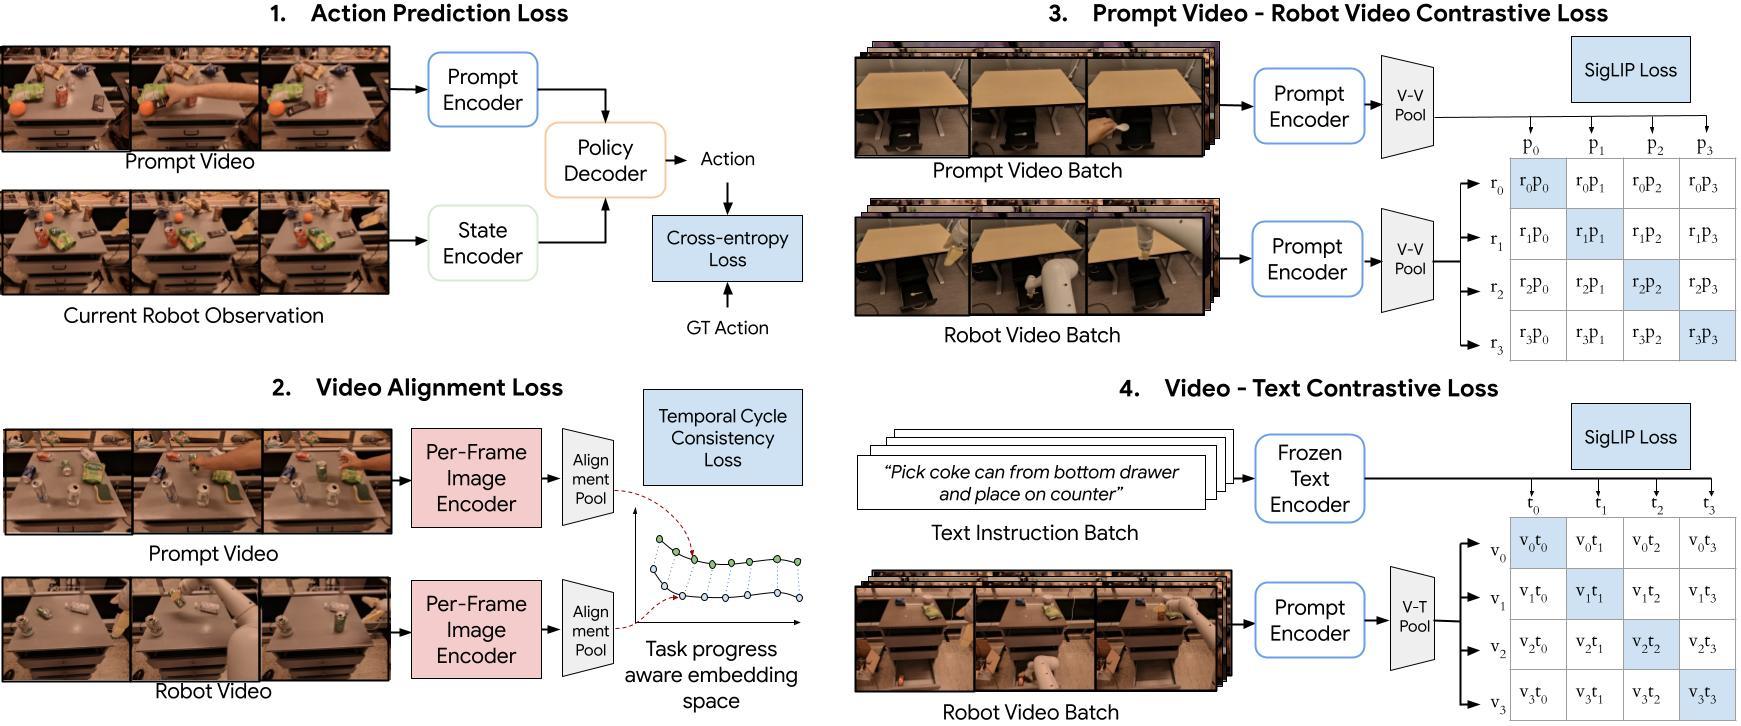
\includegraphics[width=1.0\linewidth]{./chapter8/media/Vid2Robot_Loss.png}
	\caption[Vid2Robot Loss]{Vid2Robot Loss \cite{?}.}
	\label{fig:Vid2RobotLoss}
\end{figure}

Vid2Robot is trained using with one main loss and three Auxiliary losses to encourage alignment between the prompt and robot video representations, see Figure~\ref{fig:Vid2RobotLoss}. 

\begin{enumerate}
    \item \textbf{Main Loss: Action prediction loss.}
    The primary training objective is an action prediction loss based on behavior cloning. Each action dimension is discretized into a set of bins, and the model predicts a probability distribution over these bins. Training is performed using a cross-entropy loss between the predicted distribution and the ground-truth action label. This loss supervises the entire architecture, including the Prompt Encoder, State Encoder, Cross-Attention Fusion module, and Action Decoder.

    \item \textbf{Auxiliary Loss: Temporal video alignment loss.}
    The temporal video alignment loss enforces temporal alignment between the  task progress across and the prompt video. For a given frame in the prompt video, a corresponding frame in the robot video is identified using a soft nearest-neighbor matching procedure. The matching process is then Cycle back finding for the soft-nearest neighbor found in robot video, the soft-nearest neighbor from the prompt video, which should be the same.
    The loss minimizes the distance between the circle-back frame and original prompt frame, thereby enforcing temporal consistency across both domains.

    \item \textbf{Auxiliary Loss: Contrastive loss between the prompt and robot video performing the same task.}
    This loss encourages that videos showing the same motion or interaction, such as reaching, grasping, or rotating are similar represented in the embedding space.
    First, an attention pooling layer aggregates the video features into a single embedding for each prompt and robot video. A SigLIP contrastive loss is then applied to these embeddings, promoting similarity between videos that demonstrate the same task. As a result, the model learns visual task semantics in a self-supervised manner.

    \item \textbf{Auxiliary Loss: Contrastive loss between a prompt and robot video with the language embedding.}
    The video-language contrastive loss aligns visual representations with their corresponding language descriptions. Specifically, a SigLIP contrastive objective is applied between prompt token embeddings, produced by the Prompt Encoder and language instruction embeddings associated with the demonstrated task. This encourages videos and their textual descriptions to occupy similar regions of the embedding space, allowing the model to associate visual observations with object and action semantics. Although language information is only used during training, this alignment improves text-conditioned generalization and semantic understanding.

\end{enumerate}

The losses are fused equally with the formular:
\[
L_{\text{total}} = \tfrac{1}{4}\big( L_{\text{action}} + L_{\text{video alignment}} + L_{\text{video contrastive}} + L_{\text{video-text contrastive}} \big)
\]




\subsection{Training Dataset}
\begin{figure}[!ht]
	\centering
	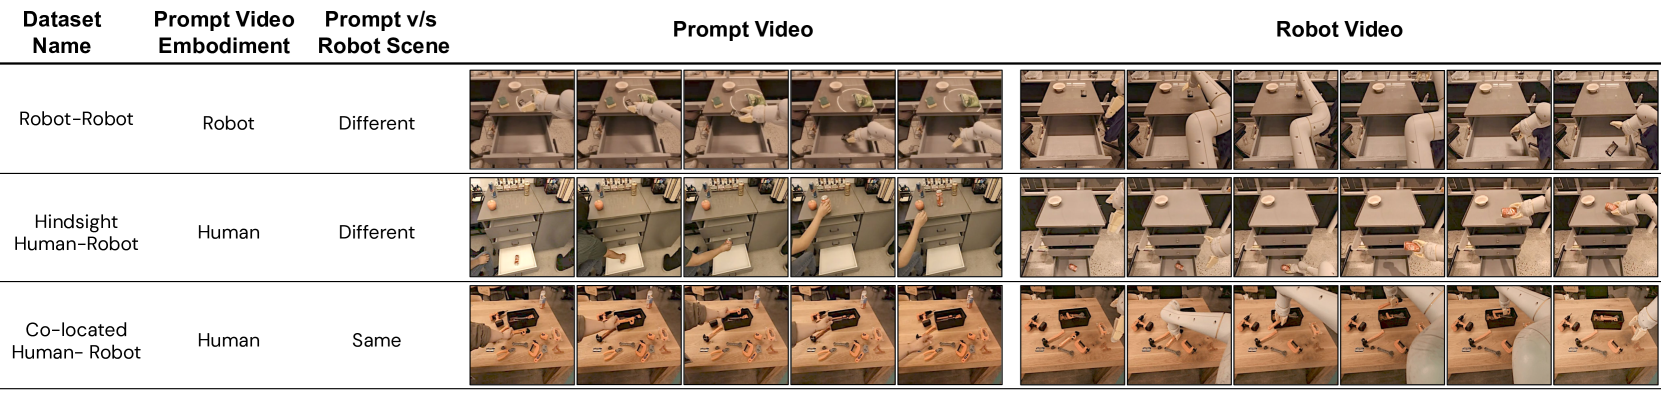
\includegraphics[width=1.0\linewidth]{./chapter8/media/Vid2Robot_Datasets.png}
	\caption[Datasets used to train Vid2Robot]{Datasets used to train Vid2Robot \cite{?}.}
	\label{fig:Vid2RobotDatasets}
\end{figure}
Vid2Robot requires paired prompt videos and robot trajectories performing the same task and is trained with three different dataset categories, see Figure~\ref{fig:Vid2RobotDatasets}.

The three datasets are:
\begin{itemize}
    \item \textbf{Robot-Robot:} Dataset with robot prompt videos and robot trajectories performing the same task. 
    
    \item \textbf{Hindsight Human-Robot Dataset:} Dataset of human demonstrations of manipulation tasks, which are paired with corresponding robot trajectories that perform the same tasks. The human demonstrations are collected with high variablity, for example using left/right hand, individual motion styles, different speeds, randomized robot camera angles.
  
    \item \textbf{Co-located Human-Robot Dataset:} Dataset of humans and robots performing the same task in the same physical workspace.
\end{itemize}
The training corpus contains approximately 100k robot-robot videos and 10k human-to-robot demonstrations. Over 90 percent of the data are robot-robot pairs, and is collected from public avialable sources.




\subsection{Summary}
Vid2Robot is trained on a large-scale video dataset of human manipulation tasks, allowing it to generalize to a wide range of unseen tasks and environments. 
The experimental results demonstrate that Vid2Robot can successfully perform various manipulation tasks, such as object picking, placing, and tool use, by directly learning from robot or human video demonstrations. 
% This approach significantly reduces the need for manual task specification and allows robots to learn from the rich visual information present in human demonstrations, paving the way for more intuitive and efficient robot learning in real-world scenarios.

\section{Paper - ORION: Vision-based Manipulation from Single Human Video with Open-World Object Graphs}
\section{Paper - Learning an Actionable Discrete Diffusion Policy via Large-Scale Actionless Video Pre-Training}

\section{Paper - Learning Video-Conditioned Policies for Unseen Manipulation Tasks}
  % % \chapter{Experiments on the Real Robot}
\chapter{Real Robot Experiments}
\label{chap:ExperimentsOnARealRobot}
\minitoc


The second part of this work will focus towards a practical implementation of an open-source \ac{IL} approach on a real robotic system. The goal is to gain hands-on experience with the challenges and opportunities when setting up a connection to a real robot. This includes how to connect the robot with a workstation and how to control the robot from the workstation.
%  and what additional code is needed to adapt a model to our specific robot. 
The goal was to implement a simple and easy-to-use pipeline for robot communication, designed such that only the robot model needs to be replaced. 
% This includes a camera setup with calibration to capture the robot's environment and provide the necessary visual input for the model.
The overall setup is designed to be modular and extensible, enabling straightforward integration of different robot models and their respective software dependencies.
The full pipeline to setup and run a robot model on a robot is as follows:
\begin{enumerate}
    \item Setup Connection between PC and Robot. 
    \item Setup the control protocols, for controlling the Robot via PC (for example within a Python script~\cite{WelcomePythonorg2026}). There exists two different control protocols: 
    \begin{itemize}
        \item RTDE: Direct control Interface provided by Universal Robots~\cite{RealTimeDataExchange}.
        \item ROS 2: A popular high-level open-source framework for controlling different robots with the same Interface~\cite{ROS2Documentation}.
    \end{itemize}
    \item Camera Setup and Calibration.
    \item Implementing the robot model on the PC and adapt it to the UR5e.
    \item Testing the robot model and evaluating the performance.
\end{enumerate}

\paragraph{Robot Hardware}
For experiments, the UR5e Robot Arm~\cite{UserManualUR5e} from Universal Robots will be used, see \autoref{fig:UR5eRobotAmberg}. 
It is a collaborative robot (cobot) designed for safe human-robot interaction. The UR5e provides a versatile and user-friendly 12 inch touchscreen interface for controlling and static programming the robot. The Gripper 2F-140 from Robotiq was used, which has a payload of 2.5 kg and a stroke of 10 to 125 Newton~\cite{AdaptiveGrippersRobotiq}. 

\begin{figure}[!ht]
	\centering
	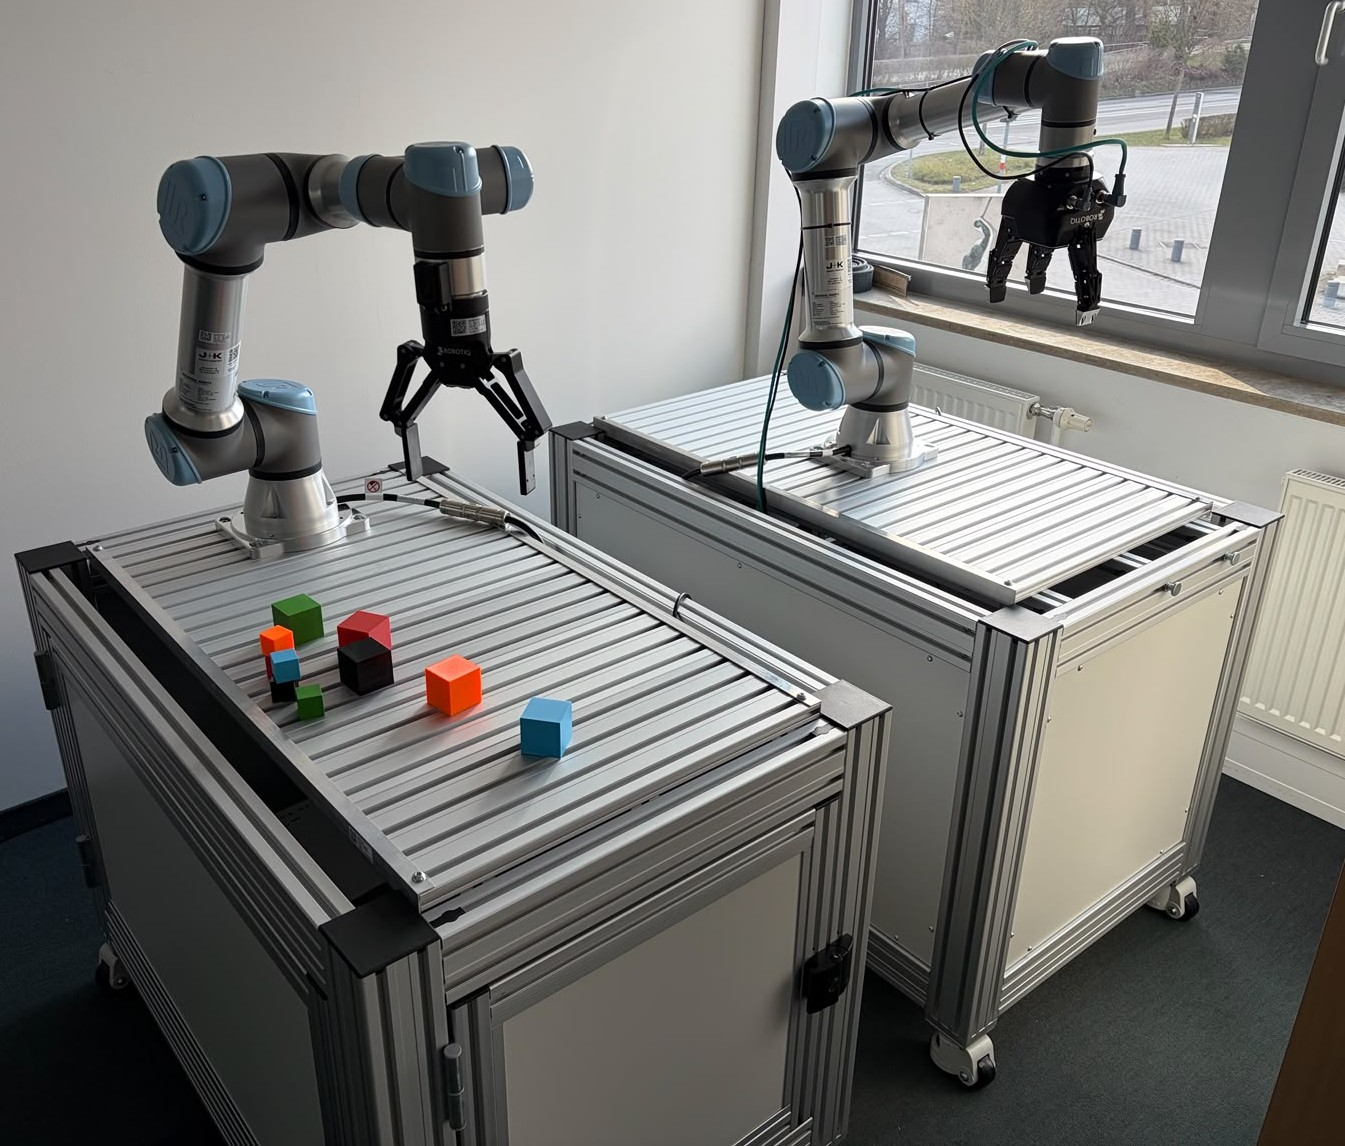
\includegraphics[width=0.6\linewidth]{./chapter9/media/UR5eRobotAmberg.jpeg}
	\caption[UR5e Robot from Universal Robots]{UR5e Robot from Universal Robots: This UR5e robot was used for experiments.}
	\label{fig:UR5eRobotAmberg}
\end{figure}


In~\autoref{tab:UR5eSpecifications} some specifications of the Robot are listed. 
\begin{table}[h]
    \centering
    \renewcommand{\arraystretch}{1.3}
    
    \begin{tabular}{|>{\raggedright\arraybackslash}m{4.6cm}|>{\raggedright\arraybackslash}m{4.3cm}|}
        \hline
        \rowcolor{blue!10}
        \multicolumn{2}{|>{\centering\arraybackslash}m{9.5cm}|}{\rule{0pt}{3ex}\textbf{Robot:} UR5e Robot Arm from Universal Robots\vspace{1ex}} \\
        \hline
        Degrees of freedom & 6 rotating joints \\
        \hline
        Joints speed & 180°/s \\
        \hline
        Payload & 5 kg  \\
        \hline
        Reach & 850 mm \\
        \hline
        Weight & 12 kg \\
        \hline
        Materials & Powder coated steel \\
        \hline
    \end{tabular}
    \caption{Specifications of the UR5e Robot Arm. Source:~\cite{UR5e_2}}
    \label{tab:UR5eSpecifications}
\end{table}




\section{Establishing PC-to-Robot Connectivity}
Many modern robot learning models require substantial computational resources for image processing, perception and action generation. In particular, many \ac{VLA} models rely on high-performance GPUs, such as an NVIDIA RTX 4090, to achieve (near) real-time inference. 
Due to these computational requirements, the robot model must be deployed on an external workstation, rather than directly on the UR5e robot, whose onboard hardware is not designed for executing large-scale deep learning models. In addition, some extra software is needed for running a robot model and communicating with the robot control interface, which can be easily installed on a PC. Consequently, a communication connection between the workstation and the robot had to be established, which enables the external computer to execute the robot model, send motion commands to the robot or receive sensor and state information from the robot required for closed-loop control.

To facilitate this process, a detailed \textit{setup guide} was created that documents the individual steps required to establish a reliable connection.
% between the workstation and the UR5e robot. 
The guide covers the configuration of network settings and communication ports on both devices, procedures for verifying network connectivity, the activation of Remote Control mode and required services on the robot, as well as the configuration of the External Control functionality. This includes the creation of an External Control program that must be executed on the robot before control commands can be transmitted from the workstation.






\section{Robot Control Protocols}


\subsection{ROS 2 - Robot Operating System 2}
ROS 2 (Robot Operating System 2)~\cite{ROS2Documentation} is an open-source robotics middleware framework used for building modular and distributed robotic systems. It organizes software into independent components called nodes, where each node performs a specific function such as perception, control, or planning. These nodes communicate with each other using standardized interfaces.
% , including topics, services and actions. 
ROS 2 provides the communication infrastructure that enables reliable data exchange between different parts of a robotic system. In this way, it acts as the “plumbing” layer that connects sensing, computation and actuation in robotics applications. A key advantage of ROS 2 is that it allows the same software components to be reused across different robotic platforms without requiring changes to the core code, as long as the robots support the same ROS 2 communication interfaces.
The complete ROS 2 implementation developed during this work is publicly available in the following repository:
\begin{center}
    \url{https://github.com/sweidner2001/RobotUR5e_ROS2}
\end{center}
% The complete ROS2 Repository is available under: \url{https://github.com/sweidner2001/RobotUR5e_ROS2}

The repository contains scripts and configuration files required to establish communication with the UR5e robot and to launch the corresponding ROS 2 nodes. These scripts automate the initialization process and provide a easy-to-use setup for robot control, visualization and simulation.
The ROS 2 environment integrates several commonly used robotics tools:
\begin{itemize}
    \item \textbf{RViz}~\cite{RvizMainPage} is a 3D real-time visualization tool for ROS, see~\autoref{fig:RViz}. It provides a view of the robot model, sensors and other information in a 3D space. It can be used to display sensor data from robots, such as point clouds, camera images, robot trajectories. While RViz can be used in conjunction with Gazebo, it is not a simulation environment of itself.

    \item \textbf{MoveIt}~\cite{MoveIt2Documentationa} is a motion planning framework for robotic manipulators that computes collision-free trajectory generation and collision checking between start and target poses, see~\autoref{fig:MoveIt}. It can be used for both simulated and real robotic systems.
    
    \item \textbf{Gazebo}~\cite{Gazebo} is a physics-based simulation environment commonly used in conjunction with ROS 2 and RViz. It enables realistic simulation of robot dynamics (mass, inertia, gravity), sensors (cameras, lidar, force sensors) and the environment (collisions, friction). Gazebo provided a virtual testing environment for validating robot configurations and control algorithms before deployment on the physical UR5e robot.
\end{itemize}

\begin{figure}[!ht]
    \centering
    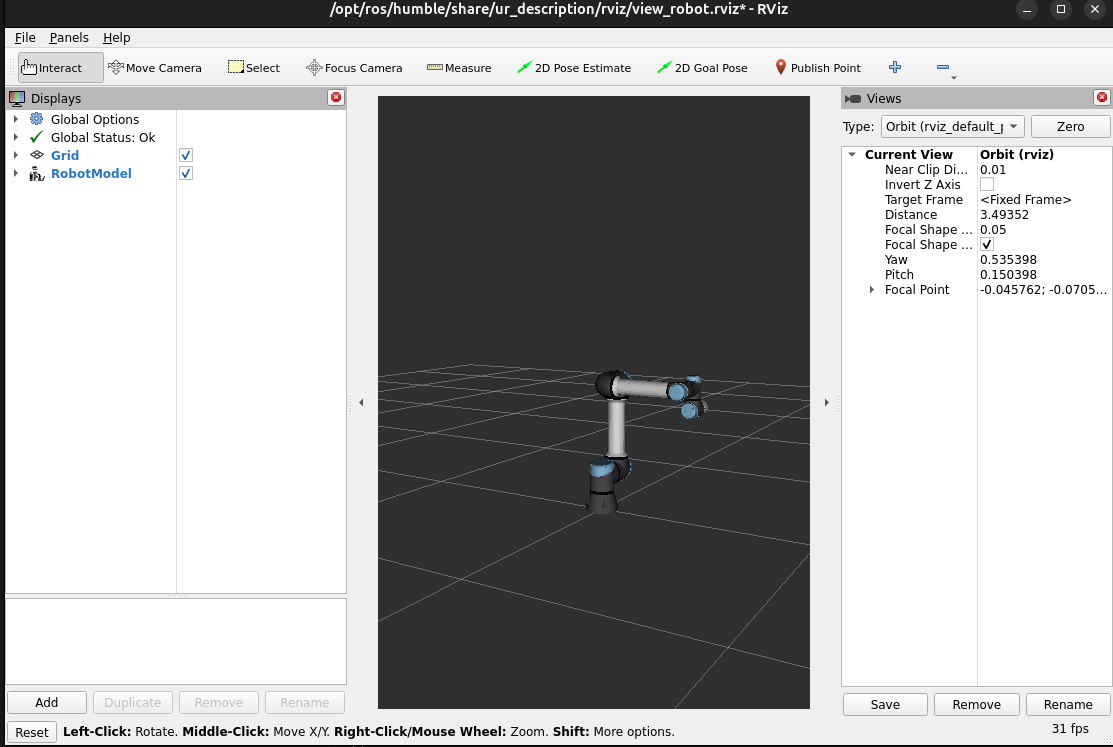
\includegraphics[width=0.8\linewidth]{./chapter9/media/Rviz}
    \caption[RViz: Visualization Tool]{RViz is a 3D real-time visualization tool used in ROS 2.}
    \label{fig:RViz}
\end{figure}
\begin{figure}[!ht]
    \centering
    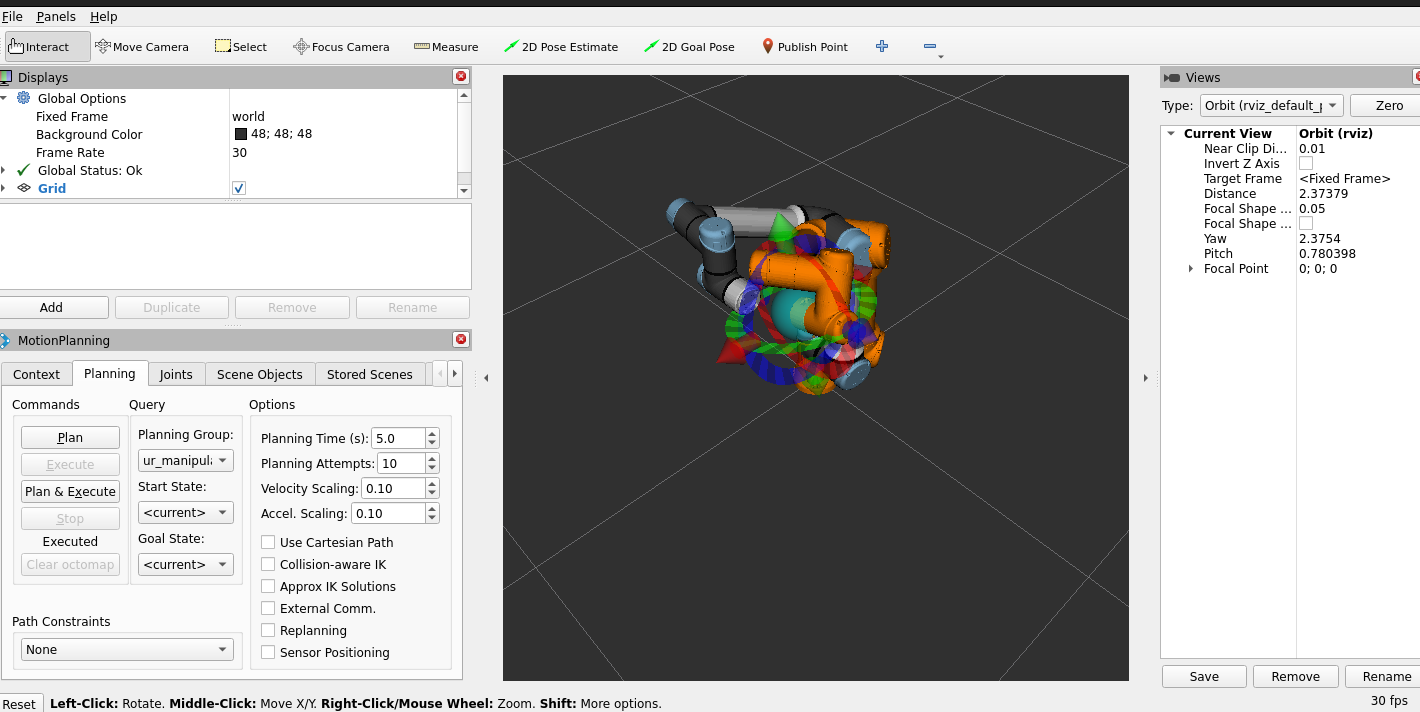
\includegraphics[width=0.8\linewidth]{./chapter9/media/RvizWithMoviIt}
    \caption[MoveIt: Motion Planning Tool]{MoveIt is a motion planning framework and here used together with RViz. The orange robot represent the target pose of the robot and within the RViz you can simulate the trajectory, which is planned by MoveIt.}
    \label{fig:MoveIt}
\end{figure}

In addition to the software implementation, comprehensive documentation was created to support the deployment of a robot model via ROS 2. The documentation describes the procedures required to establish communication with the robot via ROS 2, set the UR5e robot in External Control mode, ROS 2 commands to control the robot and commands for troubleshooting. Furthermore it explains the usage of the provided scripts and workflows for controlling the robot within both simulated and real-world environments.


\paragraph{Setup}
To simplify the development and deployment process, the ROS 2 project was implemented using a Dev Container environment~\cite{DevelopingContainer}. This approach provides an isolated and reproducible software environment, eliminating the need to install ROS 2, robot drivers and additional dependencies directly on the host system. As a result, all developers can work within a consistent environment while avoiding dependency conflicts and configuration issues.
The Dev Container provides a fully configured ROS 2 workspace tailored for Universal Robots development. It includes the required communication interfaces for the UR5e robot, as well as commonly used robotics tools such as Gazebo, MoveIt and RViz.
The Dev Container setup follows a layered workflow consisting of four main components:
\begin{enumerate}
    \item \textbf{devcontainer.json:} Defines the configuration for the development container, including user settings, mounted directories, environment variables, Visual Studio Code extensions and post-creation commands. It serves as the entry point for building and configuring the container environment.
    \item \textbf{Dockerfile:} Defines the base development environment and installs all required software packages, including the ROS 2 Distribution, the Universal Robots driver, Gazebo, RViz and MoveIt. 
    During the image build process, the script \texttt{setup\_workspace\_additional.sh} is executed. 
    \item \textbf{setup\_workspace\_additional.sh:} This script contains permanent configuration steps that become part of the Docker image and are therefore available in every container instance created from the image. You can add easily your additional setup here to extend the docker image without editing the base Dockerfile.
    \item \textbf{setup\_workspace\_temp.sh:} After the Docker image has been built successfully, the \texttt{devcontainer.json} configuration executes the script \texttt{setup\_workspace\_temp.sh}. In contrast to the permanent setup script, this script is executed each time a new container instance is created. It is intended for temporary workspace configuration, experimental package installations and project-specific modifications that should not require rebuilding the entire Docker image. 
\end{enumerate}
This separation between permanent and temporary configuration steps provides a flexible and fast development workflow while maintaining a stable and reproducible base environment.


\paragraph{Provided Scripts}
See~\autoref{tab:launch_scripts} for an overview of the provided easy-to-use launch scripts.
\begin{table}[!h]
    \centering
    \renewcommand{\arraystretch}{1.5}
    \begin{tabular}{|>{\raggedright\arraybackslash}p{4.5cm}|>{\raggedright\arraybackslash}p{10.5cm}|}
        \hline
        \rowcolor{blue!10}
        \textbf{Script Name} & \textbf{Description} \\
        \hline
        \texttt{launch\_std.sh} & Launches the UR robot driver to connect to a real UR robot. This allows for direct control of the robot through ROS 2 topics and services. If the command is successful, RViz should start and shows the robot in its current pose. If the robot is not visible, there is a connection error. \\
        \hline
        \texttt{launch\_RViz\_MoveIt.sh} & Launches the UR robot driver together with MoveIt and RViz. This allows controlling the real robot via the MoveIt planning interface in RViz. \\
        \hline
        \texttt{sim\_launch\_RViz\allowbreak\_Gazebo.sh} & Launches the UR5e simulation in Gazebo with RViz. The robot is simulated and can be visualized via RViz. \\
        \hline
        \texttt{sim\_launch\_RViz\allowbreak\_MoveIt\allowbreak\_Gazebo.sh} & Launches the UR5e simulation in Gazebo with MoveIt and RViz. In addition to the simulation, MoveIt is loaded, enabling motion planning within the simulation. \\
        \hline
    \end{tabular}
    \caption{Launch Scripts for UR5e Robot Control}
    \label{tab:launch_scripts}
\end{table}


\paragraph{Gripper Control}
To control the gripper, additional ROS 2 packages and interfaces are required, as the gripper is not directly controlled through the main robot driver. Due to missing instructions, how to control the gripper directly with a ROS 2 Node, the gripper wasn't finished implemented and is not functional yet. Some additional specific \texttt{urdf.xacro} files are needed, to connect the gripper to the robot model in Rviz. However, the ROS 2 setup provides the necessary infrastructure to integrate gripper control in the future.


\paragraph{Summary}
In summary, the ROS 2 implementation provides a comprehensive framework for controlling the UR5e robot arm from an external workstation, but there was some difficultness with the gripper control, which is not yet implemented. For this reason, the decision was made to prioritise the implementation of the RTDE interface provided by Universal Robots, as ready-made Python packages~\cite{WelcomePythonorg2026} were already available for this purpose. 
% The aim was to implement an initial working robot model as quickly as possible.






\subsection{RTDE - Real-Time Data Exchange}
RTDE (Real-Time Data Exchange)~\cite{RealTimeDataExchange} is a direct communication interface provided by Universal Robots for exchanging data between an external computer and the robot controller. It enables fast, low-latency transmission of sensor data and control commands. Compared to ROS 2, RTDE operates closer to the hardware and therefore provides higher update rates. This makes it suitable for real-time robot applications in the Universal Robots universe, where fast and reliable data exchange is required. The advantage is that RTDE is easy to set up. However, the disadvantage is that the interface must be adapted when switching to a different robot.
The complete RTDE implementation developed during this work is publicly available in the following repository:
\begin{center}
    \url{https://github.com/sweidner2001/RobotUR5e_RTDE}
\end{center}





\paragraph{Provided Scripts}
Some test scripts are provided, for example a static pick-and-place demo with three cubes, which are stacked on top and another script for the reverse process. The scripts demonstrate how to use the RTDE interface to control the robot's movement and gripper, as well as how to read sensor data from the robot. The provided code serves as a starting point for implementing more complex robot control algorithms and can be easily extended to include additional functionality or to adapt to different robotic tasks. 



\paragraph{Setup}
To simplify development and deployment, the RTDE project was implemented in a dedicated Python virtual \texttt{venv}-environment~\cite{VenvCreationVirtual}. This approach provides an isolated and reproducible setup that can be executed on any system with Python installed, while avoiding dependency conflicts with globally installed packages.

The environment can be easily set up by executing the \texttt{setup.sh} script, which automatically creates the virtual environment and installs all required dependencies for working with the RTDE interface. In addition, the script configures the project structure such that Python modules can be imported using absolute paths relative to the project root. All project scripts on every location in the project structure can be conveniently executed from within Visual Studio Code using the ``run button'' functionality, with all imports resolving correctly once the environment is activated.


\paragraph{Summary}
% The project includes several example scripts for testing and demonstration purposes. One example implements a static pick-and-place scenario in which three cubes are stacked in a predefined order, while another script performs the reverse operation.
The Project demonstrates how the RTDE interface can be used to control robot motion and gripper actions, as well as how to access and process sensor data from the robot and serves as a starting point for more advanced robot control strategies. 
% They are designed to be easily extensible, allowing additional functionality to be integrated or adapted to different manipulation tasks.




\section{Summary}
Overall, the robot setup required a significant amount of time, in particular the ROS 2 implementation, which ultimately remained incomplete and did not always operate reliably. However, by using the RTDE interface, it was still possible to quickly run a simple static pick-and-place demonstration on the UR5e robot.

Due to the limited scope of this thesis, no complete robot learning model was deployed on the UR5e, and the focus was placed on developing the foundational robot setup required for future deployment of robot learning models on the UR5e.
Nevertheless, initial considerations were made regarding the placement of cameras around and on the robot. A suitable 3D model for a camera mount on the robot was also identified for potential 3D printing.
In addition, an overview of ten promising open-source robot learning models was created, which are expected to be implemented with low integration effort in future works.






\chapter{Thesis Resumé}
\minitoc
This chapter concludes the thesis by synthesizing the key findings on video-based imitation learning for robotics and identifying promising directions for future work in advancing general-purpose robotic intelligence.

\section{Summary}

This thesis investigates imitation learning as a promising approach for enabling robots to acquire complex skills from demonstrations, with the long-term goal of general-purpose robotic intelligence.
It first introduces fundamental concepts in machine learning and robotics, with a focus on the data requirements for training generalist robotic systems and the principles how robots can be instructed to perform desired tasks. Building on this foundation, the thesis examines the paradigm of \ac{LfV}, addressing how relevant knowledge can be extracted from large-scale internet video data and transferred to robotic systems for policy learning and control. In particular, it highlights the importance of robust video understanding for interpreting human demonstrations in imitation learning settings.
Subsequently, different approaches for learning robot policies from video data are discussed, including representation learning methods, reinforcement learning-based and imitation learning approaches, hybrid techniques, and large-scale vision-language-action models. The thesis further analyzes key challenges and future research directions, emphasizing the gap between current methods and the goal of general-purpose robotic intelligence. Emerging paradigms such as diffusion-based policies, world models, and causally aware learning systems are identified as promising directions for improving generalization, reasoning, and adaptability in robotic agents.

For practical insights, selected imitation learning approaches deployed on real robotic systems are examined. In addition, a basic robotic setup for a UR5e robot arm from Universal Robots was implemented, providing a foundational platform for future experiments with robot learning models.

Overall, the thesis provides a structured overview of imitation learning and video-based robotic learning, connecting theoretical foundations with practical implementation aspects.




\section{Outlook}

This thesis provided an overview of imitation learning and video-based robot learning, as well as the practical foundations required for deploying learning-based approaches on a real UR5e robot.
The most immediate next step is the deployment and evaluation of a robot learning model on the real UR5e robot, to gain practical insights into real-world deployment and the challenges that arise in this context.
Future work should therefore focus on adapting and deploying one of the identified open-source robot models to the UR5e robot.
% , which includes writing a control script for the robot with the RTDE interface and integrating a camera system for perception of the robot. If this works, the ROS 2 implementation can be further developed and tested, to provide a more flexible and modular framework for robot control.
This process includes the implementation of a robust control pipeline using the RTDE interface, the integration of a camera system for visual perception and the development of data-processing pipelines for model inference. Once a complete perception-to-action pipeline is operational, the existing ROS 2 implementation can be further developed and tested to provide a more modular and extensible framework for robot control, simulation and experimentation.

\paragraph{Techniques \& Architectures}
Beyond the practical implementation, several research directions in robot learning remain promising. Recent architectures such as TimeSformers, Q-Formers, Action Chunking Transformers, Conditional Behavior Transformers (C-BeT) and Conditional Variational Autoencoders (C-VAE) could be investigated for their applicability to robotic policy learning. 
Additional research could investigate meta-learning approaches that allow robots to rapidly adapt to new tasks with minimal additional training. The combination of world models, causal reasoning and multimodal foundation models may represent a crucial step toward the development of more general-purpose robotic agents. The advantages and disadvantages of monolithic and compositional models can be worked out too.

Furthermore, combining traditional physics-based simulation with video prediction models represents an interesting avenue for future work. Such hybrid simulators could improve planning capabilities while maintaining physical consistency.

Another promising direction is the application of Video Question Answering (VQA) techniques to robotics. Robot systems could query video understanding models with questions such as ``Was the task completed successfully?'' to automatically generate supervision signals and evaluate task execution. While VQA has been widely used with images, but not with videos as input.



\paragraph{Learning from Videos}
An underexplored area is the use of \ac{LfV} rewards to augment offline reinforcement learning datasets. For example, an LfV policy could be refined through online reinforcement learning while using video-derived rewards to guide optimization.

As \ac{LfV} continues to gain importance, several open research questions remain. One challenge is the recovery of action information from action-free video demonstrations. Future work could systematically compare existing action representations $\hat{a} \in \hat{A}$ and evaluate their effectiveness for transferring knowledge from videos to robotic policies. Additionally, novel action representations could be developed that combine the strengths of existing approaches while reducing ambiguity during policy learning.




\paragraph{Datasets, Benchmarks and Evaluation}
Future work could also focus on the systematic analysis of existing robotics datasets and their coverage of tasks, environments and manipulation skills. Video editing and synthetic data generation techniques may provide opportunities to augment existing datasets and improve their diversity.

Finally, progress in Learning from Videos requires improved benchmark suites and evaluation metrics. Current benchmarks often focus primarily on task success rates, while future evaluations should also measure generalization, robustness, data efficiency, sim-to-real transfer performance and causal understanding. The development of such benchmarks will be crucial for the quantitative assessment of the performance of robot models and will set the future direction for research.


\paragraph{Summary}
Overall, the rapid progress in robot learning and the complementary fields of \acp{LLM} and vision models suggests that robot learning will remain a highly active research area in the coming years. Continued advances in these fields may ultimately contribute to the development of robotic systems capable of learning, adapting and generalizing across a wide range of real-world tasks.
































  
  % ... weitere Kapitel

  % Literaturverzeichnis
  % Der Name der Bibliographie Datei kann angepasst werden
  \phantomsection
  \addcontentsline{toc}{chapter}{Literaturverzeichnis}
%\bibliography{testbib}
\printbibliography
%\bibliographystyle{plain}
  \newpage

  % Anhang
  \phantomsection
  \addcontentsline{toc}{chapter}{Abbildungsverzeichnis}
  \listoffigures
  \newpage

  \phantomsection
  \addcontentsline{toc}{chapter}{Tabellenverzeichnis}
  \listoftables
  \newpage

  %\include{anhang}
\end{document}


% ToDo: unter jede Überschrift muss ein Text kommen, z.B. übersicht über das Kapitel oder die Section

% ToDo: Acronym Package